%      Copyright (c) 2014, Gyoza Book Store
%      Permission is granted to copy, distribute and/or modify this document
%      under the terms of the GNU Free Documentation License, Version 1.1
%      or any later version published by the Free Software Foundation;
%      with the Invariant Sections being LIST THEIR TITLES, with the
%      Front-Cover Texts being LIST, and with the Back-Cover Texts being LIST.
%      A copy of the license is included in the section entitled "GNU
%      Free Documentation License".

\documentclass[a4paper,10pt,twoside]{book}

\usepackage{fontspec}
\usepackage{fancyhdr}
\usepackage{listings}
\usepackage{hyperref}
\usepackage{graphicx}
\usepackage{xeCJK}
\usepackage[dvipsnames]{xcolor}
\usepackage{array}
\usepackage{makeidx}

\usepackage{layout}
\usepackage{pifont}
\usepackage{amsmath}
\usepackage{mflogo}
\usepackage{metalogo}

\usepackage[margin=2cm]{geometry}

\parindent=0pt
\setCJKmainfont{TW-Sung}
\setmainfont{Noto Sans Mono}
\makeindex

\hypersetup{
  backref,
  unicode=true,
  bookmarks=true,
  pdfauthor=Cyril Huang,
  colorlinks=true,
  breaklinks=true,
  hyperfigures=true,
  pdfstartview=FitH,
  linkcolor=blue
}

\lstloadlanguages{bash,[ANSI]C,[gnu]make}
\lstset{basicstyle=\ttfamily\small,
    keywordstyle=\color{blue}\bfseries
}

\pagestyle{fancy}
\fancyhead[RO]{\small\bfseries\rightmark\ \ \thepage}
\lfoot{餃子出品必屬佳作}
\cfoot{}
\rfoot{}

%  \includegraphics{images/gyoza.eps}
  
\title{自由的軟體開發工具v2}
\author{
  cyril\_huang@gmx.com\\
  餃子出版社
}
\begin{document}
  \maketitle
  \tableofcontents
  \newpage
  就像傳統工業工程上的製程一樣,軟體工業也有他的製作流程與管理,這些流程所
  需要的管理必須有工具來執行。
  \\\\
  以我們公司來說,我們還包括了opensource的asset管理,主要是現在已經沒有人在
  從頭開發所有的軟體了,所有的embedded系統已經全部走向Linux/BSD了,大部份系
  統通通都是拼裝出來的,裡面全都是opensource的套件,這裡面的法律跟license
  遊戲規則是必須遵守的,跟公司利益有衝突的都必須小心,所以也有這asset管理。
  不過有的管理軟體是公司內部自己實作的。
  \chapter{文字編輯器}
  很久以前我剛接觸電腦時,看到入門的人煞有其事的介紹editor,文字編輯器,我想這
  有什麼好講的,不就打打字後存檔嗎? 但是後來才發現代誌不是像憨人想得那樣而已。
  尤其對於是軟體開發者來說,editor是跟空氣一樣的,先來一些菜鳥觀念介紹
  \\\\
  基本電腦文件觀念
  \begin{itemize}
    \item 文件內容只暫存在記憶體buffer中。存檔時才會把buffer東西寫到硬碟去。
    \item 檔案真實面貌裏面有很多看不見的字元, tab, space, 換行LFCR等等,
      其中要小心的是換行字元,dos/windows是\verb=\x10\x13, unix下只有\x10=。
    \item 命令模式與編輯模式是標準傳統都會有的編輯器兩個模式,一個用來做命令,
      例如存檔,開檔,copy/paste,移動游標,一個是真正寫作。兩個模式間需要特
      殊按鍵切換,通常就是ESC。
  \end{itemize}
  程式師的編輯器
  \begin{itemize}
    \item indentation : 這是縮排對齊的一個單位。在傳統c中以tab鍵為單位。但很
      多程式語言就不一定,編輯器應該要有快速indentation的使用鍵。
    \item variable searching: 編輯器能對定義的變數做搜尋。
    \item syntax validation: 能對程式語言語法做顏色表現,也能偵測語法錯誤。
    \item IDE and outside command: 能夠使用外部工具做很多開發到測試流程的整合。
    \item setup and plugin: 有特殊變數與語法提供給使用者添加功能。
  \end{itemize}
  特殊鍵與unix習慣
  \begin{itemize}
    \item emacs / vi習慣,GNU有個readline
      library常被很多軟體使用,他提供的一些移動快速鍵,例如ctrl-e到行尾,ctrl-k
      殺掉整行等等常被很多軟體使用,同樣vi這個編輯器有很多使用鍵也有他的習慣,
      總之兩種快速鍵系統都有人用。
    \item / 搜尋鍵是vi使用的,在firefox或一些軟體中也會使用。
    \item regular express 代表鍵,unix 世界中,regular express 是一種用某種字元
      代表特殊意義的表示手法。例如\verb=^=表行首,\verb=$=表行尾。 這也常出現在
      一些軟體快速鍵中。
    \item Meta key 古早 Sun 鍵盤有個菱形方塊鍵,此為 Meta 鍵,PC 鍵盤中常以左Alt
      代表。 一些快速鍵以 Meta key 搭配其他鍵形成, 像\verb=M-F, M-%=。
  \end{itemize}
  上手前準備
  \begin{itemize}
    \item 英文打字一定要會,左右兩手手指放在asdf  jkl;上面控制a-zA-Z0-9。
    \item 免費英打遊戲可以去網路上找很多,要能盲打。
    \item 到最後,連中文輸入都盲打。
  \end{itemize}
  以上有些東西都是慢慢習慣的,一開始可能覺得很多,但最後就是習慣知道有哪些,
  這沒辦法快,只能慢慢才知道。

  \section{vim}
    本來在學校是用emacs的,後來到公司後,大家都用vi,還是傳統的vi,我很快就
    改用vi,到現在已經完全變vim了,vim的好處就是兩隻手永遠都在asdfjkl;上面。
    \begin{verbatim}
一。從命令到編輯模式
a	:將游標放到目前游標後一個字元,開始文字編輯模式。append
i	:將游標放在目前游標位置,開始文字編輯模式。insert
o	:將游標放到下一行起始位置,開始文字編輯模式。open new line
比較常用就是i,a,o,I,A,O了,將來多試幾次就好了,就很熟悉了。

二從編輯到命令
ESC	:沒事多按逃脫鍵,有益身體健康。

三命令模式中的其他命令
在命令模式中的按鍵就很多了,這些需要好好熟練一下了。
在vi命令模式裡面,有的按鍵按完後他還是在命令模式,有的改個字元或copy/paste後
又回到命令模式,有的就一去不回頭變成文字編輯模式了。
有些按鍵會把你原本想改的內容做特殊的定位,例如要改個word,也會把你帶離命令模式

檔案
:q		離開vi
:e xxxx		編輯xxxx
:w		存檔
:w xxxx		另存檔案xxxx
:q!		不存檔強迫離開
:w!		強迫存檔
:wq		存檔與離開

游標移動
h,j,k,l		往左,往下,往上,往右
0		到行首
$		到行尾
^		到這行的第一個非空白字元

w,W		到下個字, 到下個非空白的字
b,B		回上個字, 到上個非空白的字
e,E		到這個字的字尾, 到下個非空白的字字尾

Ctrl-F ,Ctrl-B	往後一頁,往前一頁
gg              表示檔頭
G		到檔尾
:n		到第n行 (所以到檔頭就是:1)
Ctrl-G		顯示第幾行
J		合併兩行

搜尋與取代
/
/pattern        尋找pattern
?pattern        往上尋找pattern
n               再往下尋找
N               再往上尋找
*               目前游標下的字串尋找
#               跟 * 一樣,只是往上找
:s/pattern/str/cgi
                搜尋pattern取代str
                其中:跟s間是指定範圍(range),沒設就是游標這行 
                1,10 表示 1-10行
                %    表示整篇
                最後cgi
                c 表示confirm尋問
                g 表示global全部
                i 表示ignore不分大小寫

常用字元字串處理
cc              改變整行
dd              砍掉整行
yy              拷貝整行(yank whole line)
p,P             貼上(paste)你最近砍掉或拷貝的

cw              改變一個字
d$              砍到行尾
ye              拷貝到這個字尾

r,R             取代一個字元, 取代整行
u,U             undo 最後修改,UNCHANGE整行
x,X             砍一個字元, 往回砍個字元(等於按backspace)

重複的處理
.               重複剛剛的命令或輸入

indentation
>>              往右一個indent
<<              往左一個indent
=               這行indentation
15==            15行indentation
gg=G            表示檔頭到檔尾做一次indent

大小寫變換
~               大小寫互換
3~              三個字元變換大小寫
VIM的大小寫變換
guw             整個字小寫
gUw             整個字大寫

這些試試看
ce, 3x, 5dd, 10w, d0, y$, 5G
	  
vim的多檔與多窗
:set hidden     這設定buffer被改動後,能夠先不儲存而換到別的buffer去
:e xxx          編輯xxx
:buffers        列出所有編輯檔
:bn             n是數 b1 b2 b3....表是開第n個buffer
:bdn            n是數:bd1 :bd2 表示殺掉第n個buffer 

:new            一個水平新窗
:vnew           開個垂直新窗
:only           只留一個窗窗

C-w j k h l     移到下 上 左 右 窗去
C-w w           到下個視窗
C-w c           關掉窗子
\end{verbatim}
    \subsection{vim小技巧}
      以上基本使用,熟悉一個下午就可以,除了基本使用外,有些使用如下
      \subsubsection{syntax color}
      \begin{verbatim}
:syntax on
      \end{verbatim}
      設定程式語言語法顏色,不過我剛開始工作時,資深工程師連這個都不用的。
      非常傳統的unix/vi。他們腦袋真的非常仔細,不需要花俏的東西。

      \subsubsection{顯示行號}
      \begin{verbatim}
:set number
      \end{verbatim}
      在遠距開會除錯時用來跟同事溝通

      \subsubsection{fold}
      程式常是小單位組成,最常見的就是一個 block ,由大括號 \{ \},包住,
      fold 是合併 block 內容成一行,讓整個檔案看起來是大塊邏輯組成即可。
      但有時自動幫我們做這些也很煩,要開開關關
      \begin{verbatim}
za    toggle 開變關,關變開
zo    open
zc    close
zA    這三個跟上面三個一樣,只是作用在檔案全部
zO
zC
      \end{verbatim}
      fold 方法有 manual, indent, syntax
      \begin{verbatim}
:set foldmethod=indent
:set foldnestmax=10
:set nofoldenable
:set foldlevel=2
      \end{verbatim}
      \subsubsection{tag symbol searching}
      用ctags命令對一堆c sources產生tag 檔,就可以跳來跳去想看的變數 symbol。
      \begin{verbatim}
      $ ctags -d -t -w `find . -name "*.[ch]"`
      $ find . -name "*.[ch]" | xargs ctags -a -d -t -w
      或者
      find . -name "*.[ch]" > files
      find /usr/include >> files
      ctags -L files
      \end{verbatim}
      -d 表示 \verb=#=define的macro, -t 表示typedef的也放進tags,
      -w 表示不要warning.
      \\\\
      幾個重要命令:
      \begin{itemize}
        \item ta myvar 跳到myvar這個tag
        \item ts myvar 列出有所有myvar tag的檔案。
        \item pop 跳回去原來地方。
      \end{itemize}
      幾個重要快速鍵:
      \begin{itemize}
        \item ctrl-] 跳到游標指的symbol,
        \item ctrl-T 跳回去原來地方。
        \item g ctrl-] 列出所有的symbol的檔案讓你選
        \item \% 跳到相對應的 block 起始或結尾,通常我們 function, for, if
          起始結尾都是 \verb={ }= 所以用 \% 可以跳到相對應的這兩個地方。
      \end{itemize}
      還有
      \begin{itemize}
        \item gd 表示尋找目前游標下字串的原始local變數
        \item gD 大寫D表示全域變數尋找
      \end{itemize}

      \subsubsection{external command}
      例如使用:!ls來使用ls命令。使用:make 來做 make 。當用 make 時,cn
      與 cl 是列出錯誤訊息並跳到發生錯誤行的命令。

      \subsubsection{autocomplete}
      ctrl-n 可以 autocomplete, autofill 自動補全打一半的字,不過這只是根據
      現有檔案內有的字串,要像一般 IDE 那樣,必須裝特別 vim plugin 才行。

      \subsubsection{vimdiff}
        同時編輯兩個檔案並用顏色標出兩者不同處,這通常是用來解
        branch merge後conflicts時所用。使用\verb=[c ]c=跳到下一個兩邊不一樣
        的地方。解完後,顏色不同的地方會自動消失,我跟同事使用時,同事非常
        驚豔,想說怎麼這麼好用,完全是他們不會用而已。
      \subsubsection{.vimrc}
      vim有豐富的內部變數設定,也有條件式的script可以使用與設定變數,像之前
      的syntax on這個就是命令之一,只是冒號: 都不用打了。所以可以把這些設定
      寫到\$HOME/.vimrc去,則整個起來的環境就是個人使用環境。
      \\\\
      一個簡單的.vimrc
      \begin{verbatim}
if has('syntax') && (&t_Co > 2)
	syntax on
endif

set autoindent
set title
set ruler
set hidden
set fileencodings=utf-8,big5
set fileencoding=utf-8
set encoding=utf-8
function Setsts()
  if &sts == 0
    set sts=2 sw=2
    set expandtab
  elseif &sts == 2
    set sts=4 sw=4
    set expandtab
  elseif &sts == 4
    set sts& sw&
    set noexpandtab
  endif
endfunction
map <F2> :call Setsts()<BAR>set sts?<CR>
map <F3> :set paste!<BAR>set paste?<CR>
map <F4> :set hls!<BAR>set hls?<CR>
map <F5> :bp<CR>
map <F6> :bn<CR>
map <F7> g^]
map <F8> ^T

if has("autocmd")
  filetype plugin indent on

  autocmd FileType text set sts=2 sw=2 expandtab textwidth=78
  autocmd FileType sh set sts=4 sw=4 expandtab
  autocmd FileType perl set sts=4 sw=4 expandtab
  autocmd FileType python set sts=4 sw=4 expandtab
  autocmd FileType php set sts=4 sw=4 expandtab
  autocmd FileType spec set sts=4 sw=4 expandtab
  autocmd FileType c set sts=4 sw=4 expandtab cindent
  autocmd FileType javascript set sts=2 sw=2 expandtab
  autocmd FileType vim set sts=2 sw=2 expandtab
  autocmd FileType rst set sts=2 sw=2 expandtab
  autocmd FileType tex set sts=2 sw=2 expandtab
  autocmd FileType sgml set sts=2 sw=2 expandtab
  autocmd FileType html set sts=2 sw=2 expandtab
  autocmd FileType conf set sts=2 sw=2 expandtab
  autocmd FileType yang set sts=2 sw=2 expandtab autoindent

  autocmd BufReadPost *
    \ if line("'\"") > 0 && line("'\"") <= line("$") |
    \   exe "normal g`\"" |
    \ endif

endif " has("autocmd")
      \end{verbatim}
      其中那些set就是設定變數值,沒有等號的就是設true。sts是softtabstop表示按
      tab時是跑幾格,sw是shiftwidth,表示使用\verb=>> <<= 時,indent時,是跳幾格。
      expandtab是說如果有8個space時,要不要把他自動變成一個tab表示。
      而其中很有用的就是map這個設定快速鍵使用。這個必須:help map就可以看到文件
      。通常搜尋vim網站,可以看到很多人寫的小設定了,可以直接拿來使用就好。
      \\\\
      其中F7與F8用上了特殊鍵ctrl,但\verb=^] ^T=兩個值是不能用打字ascii方式輸入
      ,而必須真的是這兩個鍵的binary值,所以必須ctrl-v ctrl-]輸入\verb=^]=,
      ctrl-v ctrl-T輸入\verb=^T=。

  \section{emacs}
    emacs的就稍微放一下以前寫的命令小抄,我已經完全忘光不用emacs了。不過資深白人
    同事,使用 emacs 都嚇嚇叫,出神入化
    \begin{verbatim}
檔案
C-x C-c		:離開 emacs
C-x C-f		:開檔
C-x C-s		:存檔
C-x C-w		:另存新檔

游標移動:
C-a		:移到行首
C-e		:移到行尾
M-f		:向後移一個字
M-b		:向前移一個字
HOME		:移到檔頭
END		:移到檔尾
M-m		:移到這行第一個字元

常用的鍵
M-x		:執行一個emacs命令
C-g		:離開一個emacs命令
C-_		:UNDO
C-s		:搜尋  一直按一直往下找
C-r             :往上搜尋
M-%		:搜尋與替代(按!全部換掉,要不,會一個一個問按y/n回答)
M-C-s		:regular express 搜尋

M-DEL		:往前砍個字
M-d		:往後砍個字
C-k		:砍掉游標後所有字
M-t		:轉換兩字
C-x C-t		:轉換兩行
    \end{verbatim}
    一般說來在X 視窗下,我們可以用滑鼠就可以標示文字了,現在通常有兩個 buffer,
    一個是Window Manager 像 gnome, kde 提供的 clip board buffer, ctrl-c,
    ctrl-v,另一個是原本 X 提供的, 只要用滑鼠左鍵標好,可以按 shift 鍵調整,然
    後用滑鼠中鍵就可以paste了。 這如果按著 shift 鍵跟滑鼠左鍵可以更精確控制。
    emacs的區塊沒有所謂的column mode的區塊。
    \\\\
    區塊的標記:
    \begin{verbatim}
C-SPCE = C-@	:開始區塊標示,然後移動游標
		:如果想看到反白請先下emacs 命令"transient-mark-mode"
		:但如果用了這個,滑鼠的左鍵標示就看不到反白了喔。
C-x h		:標示整個編輯區(就是整個檔案)
C-w		:砍掉標示的區塊(用滑鼠右鍵按兩下或按del - 這個要20版以上的才有)
C-y		:把剛剛砍掉的或在區塊中的文字回存(也可以用滑鼠中鍵)

多檔與多窗
C-x 5 2		:開一個新窗子在新的frame
C-x 3		:開新垂直窗子在同一個frame
C-x 1		:只留一個窗子
C-x o		:改到其他(other)窗子
C-x b		:改到其他buffer(編輯區)
C-x k		:kill掉目前編輯區
C-x C-b		:列出所有編輯檔案

基本巨集
C-x (		:開始紀錄你所按的鍵
C-x )		:結束你所紀錄的鍵
C-x e		:執行剛剛紀錄的所有組合按鍵
M-n C-x e	:執行n遍剛剛的按鍵

TAB		:對齊indent
M-C-\		:對區塊做一次程式的對齊(indent)
\end{verbatim}
同樣也有 etags 來做 symbol 跳躍,
\begin{verbatim}
$ etags -d `find . -name "*.[ch]"`
$ find . -name "*.[ch]" | xargs etags -a -d
$ find . \(-name "*.[ch]"\) -o \(-name "*.cc"\) | xargs etags -a -d --c++
\end{verbatim}
使用 hot key 來搜尋
\begin{verbatim}
M-.		:找一個TAG也就是symbol(就是一個變數或函式名)
C-u M-.		:繼續找,因為這個不是你想要的。
M-*		:回去剛剛按尋找TAG的起始處。
\end{verbatim}
  emacs 也一樣跟外部 make 等等都有很好的連結,只是這麼多年後,我已經忘了。

  \section{其他}
  主要是 GUI IDE (integrated development environment) 的 programmer editor,
  通常這種 IDE 也會是個 project 管理軟體。因此使用一開始會有開 project 的
  概念與 workspace 目錄, 資訊檔 template 的幫你建造。設定中,其實跟上面 vim
  所有的是差不多觀念,但多了一些方便新手使用,就是
  \begin{itemize}
    \item project 管理,名稱,作者,版本等等資訊整理。
    \item indent 這就是要注意組裡的規定,空格,tab 是幾格,tab 是8 時,
      要不要全打開成空格還是只有一個 tab 字元。
    \item Windows/Unix 的換行字元設定。
    \item searching 變數, symbol, 字串等搜尋。
    \item symbol 跳躍
    \item build/debug
    \item file browsing, 檔案總管與搜尋。
    \item autocomplete, autofill 自動補全 API, 變數。
    \item 多窗使用,能切換於多個不同像 editor, debug, command 等多視窗。
  \end{itemize}
    \subsection{eclipse}
    這是個有漂亮GUI的編輯器,寫 Java 的人會用吧,我不會寫 Java 的,但同事很
    多人用。在2000 年中期後有段時間還蠻多人用。
    主要是他能利用各路提供的plugin,做為多種程式開發的IDE。但他需要Java,
    如果是靠 Java 生態系等其他工具的人,用這個還是蠻方便的。
    \\\\
    Linux下就去下載 JRE 與 \href{https://eclipse.org}{eclipse.org},以前自己分別
    下載 eclipse 與 oracle的 jre 1.7。現在最新版的只要解開 tar.gz 檔,跑裡面的
    ./eclipse-inst 不用下載 JRE,就自動幫你下載其他需要的東西,非常好安裝。
    \begin{itemize}
      \item 裝新plugin : 現在通常都是裝一脫拉庫,所以在Help \verb=->= install
        software 下面可以給一個遠端site,跟一般使用OS的套件觀念是一樣的。在 Help
        下的 marketplace可以找到更多 eclipse 上的plugin套件。
      \item perspective : 一個整合的各種視窗集合,例如Java的perspective包含了
        檔案檢視窗,editor, 執行除錯窗等等。安裝 eclipse 事先做好的包包,會含有
        很多perspective,例如 source control 裏面的 git,或者 JUnit等。各種窗的
        出現與否也可由Window這裏面去設定。
      \item project : 各種perspective所開的project,通常就是開一個目錄,下面有
        些奇奇怪怪的conf檔與resource檔。通常有所謂 general 的 project,然後可以
        convert 成其他的 project,例如 maven project,下面會有 pom.xml 檔,如果
        是 c project 那可能會有 Makefile,總之他這 project 只是個籠統的泛稱。下
        面再由不同的目的與可能的特有檔案如 Makefile, Java ant 的 build.xml, 
        maven 下的 pom.xml 做的細部分類而已,不用被嚇到。
        project 跟 perspective 是分開來的,例如 git perspective 可以去 clone
        回一個 source,然後由 project 中去 import 進來一個 project ,然後 convert
        成別更細部的 project。
    \end{itemize}
    一樣重要的
    \begin{itemize}
      \item indentation 對齊功能 :
      \item syntax color validating :
      \item API 與 symbol searching :
      \item 外部工具使用 : 像build, debug都有外部程式來呼叫使用,所以也有一些
        像git的perspective可用與設定。
    \end{itemize}
    由於他本身已經是GUI了,所以檔案browser等功能自然都帶有了,一般設定 break
    point 的功能也是 IDE 都有的。這種GUI東西沒啥好講的,重點還是那些名詞選項
    是否真了解是什麼。

    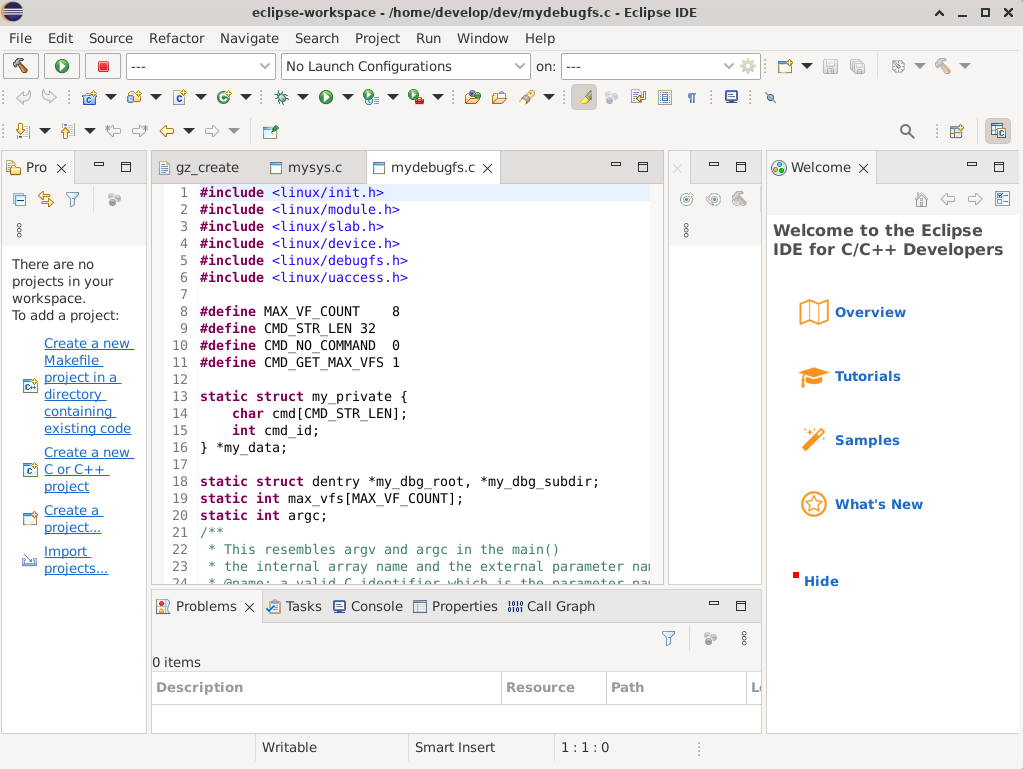
\includegraphics[width=\textwidth,height=0.6\textwidth]{images/eclipse.png}

    \subsection{vscode}
    這個 Microsoft 公司丟出來的 IDE ,後來隨著新畢業的小朋友帶進公司,很多人
    也都直接用這個,跟 eclipse 一樣,由於換組時,剛進去組裡的規矩規定環境操作
    方法,例如 source code 在哪,library 怎麼設定,參考文件都用 vscode ,所以
    我也被逼著用一下子,然後了解後,又用回熟悉的 vim, git 等命令。
    一樣可以\href{https://code.visualstudio.com/}{下載} Linux 版本。
    沒有權限的話,deb 可以用 ar 解開
    \begin{verbatim}
    ar vx code_1.86.2-1707854558_amd64.deb
    mkdir opt/vscode
    tar Jxvf data.tar.xz -C opt/vscode
    \end{verbatim}
    rpm 用 rpm2cpio 解開
    \begin{verbatim}
    mkdir -p opt/vscode; cd opt/vscode
    rpm2cpio code-1.86.2-1707854644.el8.x86_64.rpm | cpio -vid
    \end{verbatim}
    在裡面的 usr/share/code/bin 的執行檔執行。
    \\\\
    他裡面其實反而沒有 eclipse 的自創名詞,比較好懂,module 就 module, plugin
    就 plugin, extension 就 extension。
    \begin{itemize}
    \item workspace 這個是一個工作目錄,裡面有 project, source control 管理
      等資訊,而且這會跟 source control 有關,source control 通常會目錄下
      有好多支 branch ,則這樣會跟 workspace 打架,因此要特別注意使用。
    \item extension 等於是 module/plugin 我們好像一開始都會裝 ssh ,可是網路
      失敗時,他整個跳不出來,蠻爛的。另外副檔名的設定,也很誇張,內定居然
      file browser 不去讀沒支援的副檔名 extension。
    \item profile 某個大堆頭的整體設定
    \end{itemize}
    其實 microsoft 有個 packages.microsoft.com 網站,裡面的 repos 放了他們的
    Linux 軟體。

    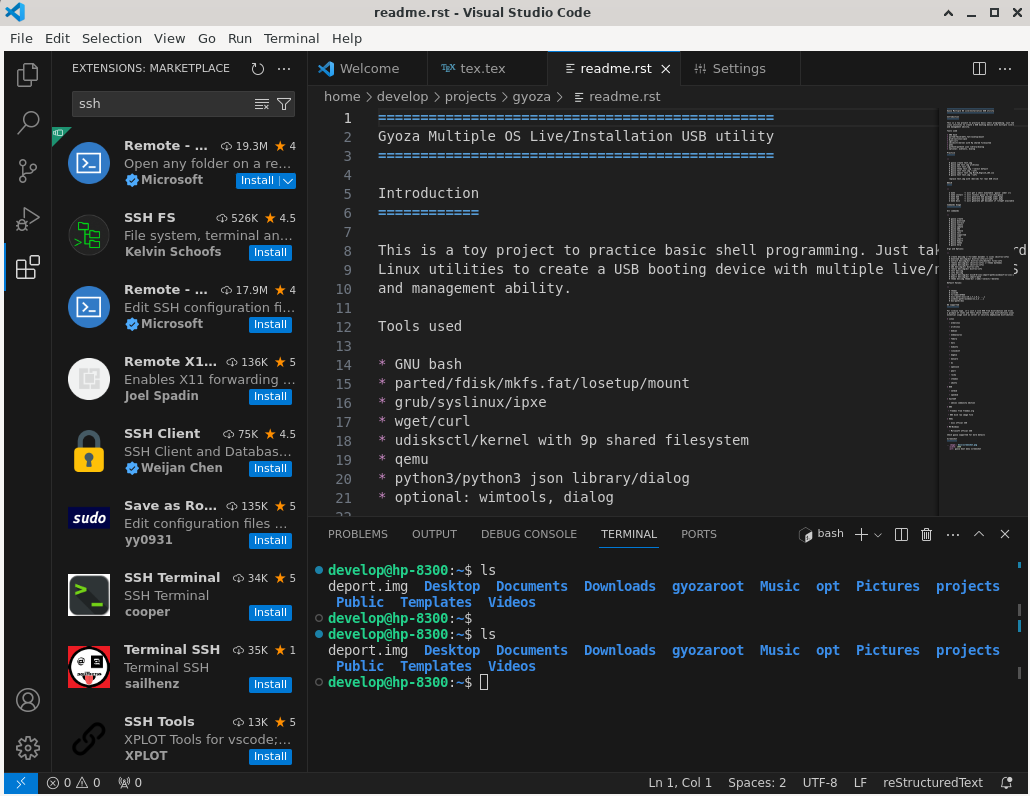
\includegraphics[width=\textwidth,height=0.6\textwidth]{images/vscode.png}

    \section{使用vim做一個IDE}
    我沒有很喜歡IDE,像 eclipse vscode,剛開始用,覺得不好用就是沒有習慣,
    真正要會用,也是真了解所有的步驟的含意,但真了解了,IDE 也不見得要有了。
    但菜鳥工程師除非是天才,不然一般人很難有習慣從心中完全想清楚規劃才 
    codeing, testing ,所以 IDE 對剛開始練習,嘗試有時還是有用。用熟練後,也
    蠻快速神奇的。做為一個IDE, 通常重要的就
    \begin{description}
      \item [file browser] \hfill \\
        可以像一般檔案夾那樣選擇檔案
      \item [include path的設定]\hfill \\
        PYTHONPATH,PERL5LIB, /usr/include, jar檔的引入
      \item [library path的設定] \hfill \\
        例如能設定PYTHONPATH, PERL5LIB, LD\_LIBRARY\_PATH,jar 檔引入,讓
        環境自動找到想用程式庫。
      \item [編譯] \hfill \\
        命令像make, java, mvn之類的呼叫,與出錯的除錯跳躍。
      \item [code completion] \hfill \\
        自動完成變數, API等的輸入。
      \item [syntax checking] \hfill \\
        語法的顏色與檢查
      \item [break point 與 run]
        能設定break point與執行程式並且一步步 trace
      \item [debug console] 
        能除錯及對於stdin/stdout/stderr的控制,通常也有 terminal 窗窗在大
        window 下。
    \end{description}
    除了可以使用.vimrc來初始vim外,.vim/plugin是個可以放特殊vim plugin的地方,
    作為一個IDE,推荐的plugin有
    \begin{itemize}
      \item \href{https://github.com/tpope/vim-pathogen}{pathogen}
      \item \href{https://github.com/scrooloose/nerdtree}{nerdtree}
      \item \href{https://github.com/ervandew/supertab}{supertab}
      \item \href{https://github.com/Valloric/YouCompleteMe}{YouCompleteMe}
      \item \href{https://github.com/scrooloose/syntastic}{Syntastic}
    \end{itemize}
    最簡單基本用法就是git下載後,把裏面的東西copy到.vim下就可以了。在vim官網中
    有一些\href{http://vim.wikia.com/wiki/Use\_Vim\_like\_an\_IDE}{介紹}

      \subsection{neovim}
      目前有一個新的 vim 替代品為 neovim,他的 IDE plugin 基本上更簡單安裝,
      \begin{itemize}
        \item \href{https://github.com/neovim/neovim/blob/master/INSTALL.md}{下載 neovim}
        \item 安裝 lazyvim plugin
        \begin{verbatim}
git clone https://github.com/LazyVim/starter \$HOME/.config/nvim
        \end{verbatim}
        \item 要花俏的外觀要裝
          \begin{itemize}
            \item \href{https://www.nerdfonts.com/}{nerd font} 這是 lazyvim
              會用到字型。選 JetBrain,在 linux 中放到 \$HOME/.fonts 並且
              mkfontscale
            \item \href{https://sw.kovidgoyal.net/kitty/}{kitty terminal},
              這是 optional 的 terminal,因為 gnome-termianl, xfce4-terminal
              都可以顯示漂亮的 nerd font。
              linux 中,export GLFW\_IM\_MODULE=ibus 然後啟動 kitty
          \end{itemize}
        \item 啟動 nvim
      \end{itemize}
      就有一個不錯的vim IDE。
      \begin{center}
      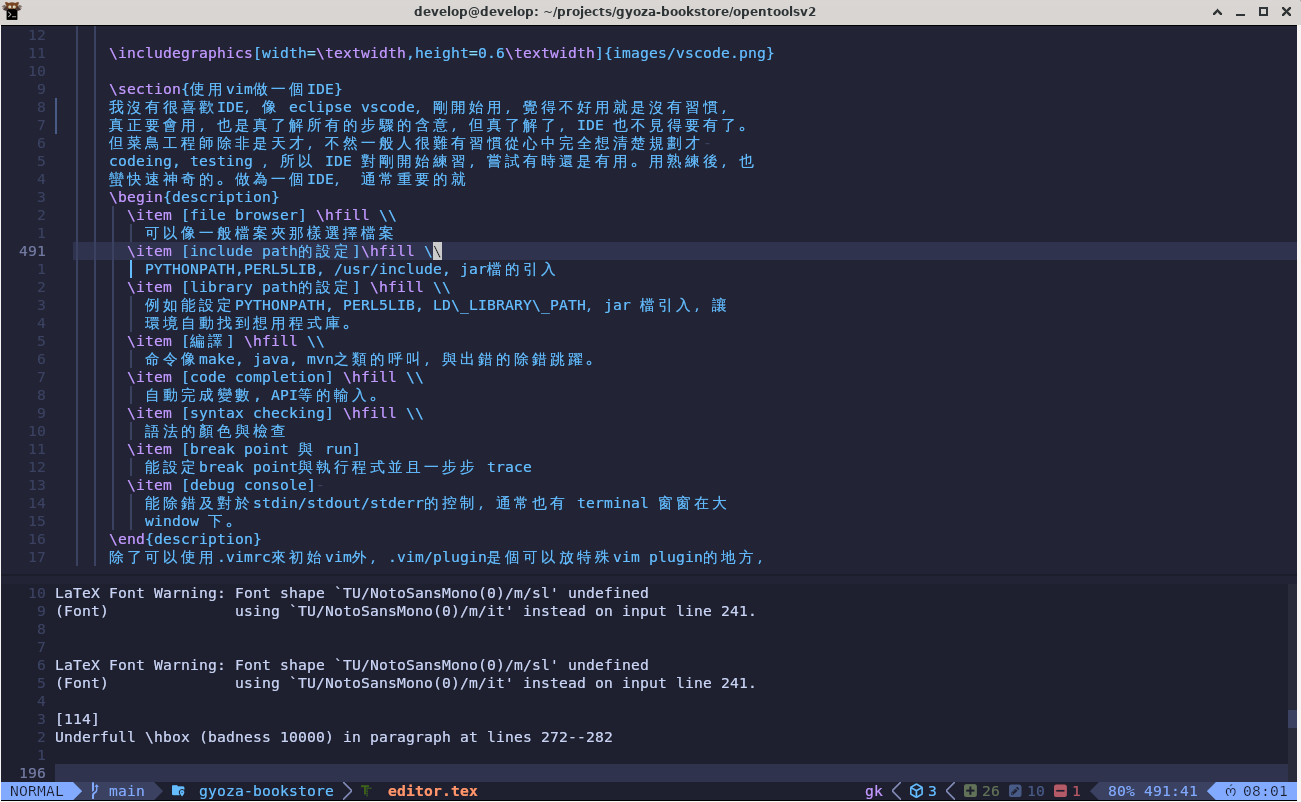
\includegraphics[width=\textwidth,height=0.6\textwidth]{images/nvim.png}
      \end{center}
      nvim 的設定主要是在 \$HOME/.config/nvim/init.lua,是個 lua script,然
      後主要安裝 lazyvim 這個簡易 plugin 就有自動補全的功能。如果要把原本
      .vimrc 的設定搬進來,在 init.lua 中使用 vim.cmd(),例如
      \begin{verbatim}
vim.cmd(set hidden)
      \end{verbatim}

    \section{其他輔助工具}
    其實shell本身就是非常強大的字串處理程式,加上sed/awk與其他工具,都能處理
    很複雜的問題了。但有些文字工具是對程式師特有的。
    \begin{itemize}
      \item grep -r pattern 搜尋子目錄下檔案裡面 pattern 的字串。解 bug 通常第
        一件事就是看錯誤訊息在哪裡。
      \item ctags/etags 建造變數,定義,函數等symbol的跳跳index。
      \item cscope 跟ctags很像,但他還能找特別的string,不光是特殊symbol。通常
        cscope/ctags是合併一起用。cscope -R -q 會產生
      \begin{itemize}
        \item cscope.out      Symbol交叉參考(cross-reference)檔
        \item cscope.in.out   反向索引檔用來做快速Symbol
        \item cscope.po.out   反向索引檔
      \end{itemize}
      要結束請按ctrl-D
      \item indent 根據自訂條件的indentation再處理。
      \item diff 與 vimdiff 比對兩個檔案的差異。
        \begin{itemize}
          \item diff -puN : print the c function and 3 lines of unified context
          \item diff -ruN : 產生一個patch檔,file.diff, patch -p1 \verb=<= file.diff;
          \item diff -yN : two column
        \end{itemize}
        vimdiff 可以直接在兩個檔案編輯,通常在解決 merge conflict 的時候很有用。
      \item patch 兩個檔案差異的對前一版的修訂。這比較重要的就是使用p0或p1選項
        ,例如source在myproj-1.0目錄,則使用diff產生的patch檔,站在myproj-1.0
        外面就是 patch -p1 \verb=<= mypatch, cd myproj-1.0後就是 patch -p0 
        \verb=<= mypatch,現在也很多用 git diff, git apply 來作業。
      \item tmux 與 screen 是在 terminal 上畫出多個窗窗工作的軟體,兩派也激戰
        很久,screen 有個好處是他同時可作 rs232 console port 的 terminal ,
        但 tmux 有很多新進處理比 screen 好。他們的主要用法是先給一個前置命令
        按鍵表示後續按鍵是軟體命令,差別就是前置按鍵
        \\\\
        tmux, 術語中, pane 表示真實切割畫面,window 表示虛擬 terminal+shell
        \begin{itemize}
          \item 開水平pane Ctrl-b " (split)
          \item 開垂直pane Ctrl-b \%
          \item 開虛擬window Ctrl-b c  (neww)
          \item 跳到下一個window Ctrl-b n (next)
          \item 跳到上一個window Ctrl-b p (prev)
          \item 跳到下一個pane Ctrl-b 上下左右
          \item 關閉pane Ctrl-b x (kill-pane)
          \item 進到命令列 Ctrl-b :  (這跟 vi 是很像,冒號後跟命令)
          \item 調整pane 大小 Ctrl-b Ctrl-上下左右
        \end{itemize}
        screen,用術語 region 表示真的切割畫面, window 表示虛擬 terminal+shell
        \begin{itemize}
          \item 開水平region Ctrl-a S  (split)
          \item 開垂直region Ctrl-a |  (split -v)
          \item 開虛擬window Ctrl-a c  (create)
          \item 跳到下一個window Ctrl-a n (next)
          \item 跳到上一個window Ctrl-a p (prev)
          \item 跳到下一個region Ctrl-a tab (focus)
          \item 關閉region Ctrl-a X (remove)
          \item 進到命令列 Ctrl-a : (這跟 vi 很像,冒號後跟命令)
          \item 列出window Ctrl-a " (windowlist -b)
          \item screen /dev/ttyS1 變成 serial port 1 的 console
        \end{itemize}
      \item a2ps 古老以前code review,我們是印出來的,現在都是線上code
        review。這在/etc/a2ps.cfg下可以全域設定。通常duplex印雙面,調整
        紙張大小letter-lj之類的。
    \end{itemize}
    \section{結語}
    不管是哪種editor,最重要的就是整組人馬是用同一種coding style, 用同一種
    indentation, 同一種換行,同一種習慣,這在將來code的維護,branch的merge
    ,開發,測試,除錯的循環中會影響效率非常的大。每個好的editor都是可以調整
    的,所以一定要把規矩講清楚,大家來遵守。至於要用 vim, emacs, neovim, 
    atom, eclipse, vscode, sublime ...其實都無所謂。

  \chapter{版本控制系統}
SRM(software revision management) 版本控制是對 source 的歷史紀錄及開發實驗的重
要工具。早期有光純local的RCS, 後來延伸的client/server CVS,有的公司內部是很
厲害的,像我們以前的版本控制是自家工程師自己寫的,後來最有名的商用是rational
clearcase 等等,隨著時代進步,很多限制與缺點都慢慢改進,目前業界用很大的是
subversion 與 git。曾經在網路看到台灣人在問這東西可以用在2,3000人的公司嗎?
基本上現在全世界的軟體業已經全部轉到 opensource 上來,
現在 embedded 系統不是 BSD 就是 Linux。幾萬人的公司在用的工具全是 opensource
工具。
\\\\
版本控制中說穿了就是graph/node理論以及多人同時處理一個檔案的data sync問題,
各家有各家的想法跟實作。基本操作都差不多,但最重要的一個觀念是版本控制不是
備份,也不是雜七雜八亂七八糟 binary的東西都丟上去,只有最原始人用editor產生
的東西,還有很多人一天到晚亂check in。那種版本紀錄就跟沒有沒兩樣,一點也沒
有意義。
\\\\
branch與merge是版本控制中最重要的部份,沒了branch/merge,那就沒有 SRM 的意義。
有人說這樣不怕檔案丟失,如果同一顆硬碟,那是一樣的,如果不是同硬碟,沒有遠端
專業大手筆的RAID, SAN, backup 等手段,也是無
意義的備份而已。以我們公司來說整個NFS系統是24小時都在運轉備份的,我們的svn
git server 都是24小時無數的 SAN/RAID/cluster的storage的。當有這些東西時,那
code 正確小心的進入 SRM 才是正確的作法(每次 code 要進去,一定是大家 review 
過的才行,如果 review 過後出問題,那 senior 的工程師就不該領那份薪水,以前
是連一個 space 空錯了,都是打回去重寫的)。
\\\\
合併重要的觀念就是以兩點的delta中產生的變化與某支中的source進行合併。
其中有兩個重要名詞
\begin{itemize}
  \item rebase/promote 傳統上爸爸到小孩稱rebase, 小孩回爸爸稱promote,
    這應該是從clearcase來的, 算是正統srm/scm業界的標準辭彙。
  \item sync/reintegrate 這相當於rebase/promote,svn提出這樣的辭彙。但有點
    不太一樣的解釋。主要在 svn 的版本編號與model有點不太一樣,沒有 rebase 
    / reparent的東西,但一樣有爸爸到小孩這件事,而且他用svn merge這樣的命令。
  \item rebase/merge 這是git提出類似rebase/promote的辭彙。
\end{itemize}
也就是說 merge 這個名詞在標準 SRM 中是很籠統的,他的定義,語法,作用其實是跟著
不同工具而有所不同,這也是一般初學者搞不清楚的地方,以為merge merge就那麼一回
事。然後看了一堆文件還是一頭霧水,svn merge 跟 git merge 跟 clearcase 講的 merge
根本就不一樣。所以如果在以下文章中我說merge,有可能我說的
就是籠統的merge (合併),請不要搞混。在真實的 implementation中,每個SRM提出的
方法或許不同,或有他實作的特殊方法,但但但...最重要的最終目的,都只是要做到
rebase/promote這兩件事。不要被其他拉哩拉雜的語彙給騙了。
\\\\
merge back的觀念在於
只要public出去server的source,就無法undo歷史,就必須merge back,並且產生一個
新歷史紀錄。所以local怎麼亂搞都無妨,但只要svn commit/git push有對外歷史紀錄,
想反悔,那就只能merge back。這都是對外歷史紀錄,必須保留。
\section{subversion}
  他有一些特點
  \begin{itemize}
    \item client / server subversion是一般的client/server,所以要有svn server
      才行。
    \item 版本號碼是所有branch同一個version space,也就是不管在哪個branch上,
      只有一個獨一無二的版號。cvs的版本號是per file的,但 svn 的版本號是
      per project
    \item 能處理binary,雖然binary檔不該進srm,但現在很多網頁的圖檔屬於binary
      檔,很多人偷懶,當然也有很多白爛的工程師亂搞,正常 binary 檔應該在 file 
      system 裏面。
  \end{itemize}
  \subsection{server建置}
  以apache +SSL 當作溝通的server,apache 需要裝dav svn模組。
  裝三個packages, libapache2-svn apache2 subversion。3個設定: httpd, dav\_svn
  mod\_ssl
  \\\\
  httpd.conf要load的模組
  \begin{verbatim}
  LoadModule dav_module         modules/mod_dav.so
  LoadModule dav_svn_module     modules/mod_dav_svn.so
  \end{verbatim}
  dav\_svn.conf檔案的設定
  \begin{verbatim}
  <Location /svn>
      DAV svn
      SVNParentPath /var/lib/svn

      AuthType Basic
      AuthName "Subversion repository"
      AuthUserFile "/etc/apache2/dav_svn.passwd"

      <LimitExcept Get Propfind Options Report>
         Require valid-user
      </LimitExcept>
      SSLRequireSSL
  </Location>
  \end{verbatim}
  authentication/authorization 用的是 apache 內部的,所以 dav\_svn.passwd 必須以
  htpasswd 去建立。最好是把 ssl enable 起來,所以在 debian 上面是把 default-ssl
  與 mod\_ssl 給 enable 起來。
  \begin{verbatim}
cd /etc/apache2/sites-enabled
ln -s ../site-available/default-ssl .
cd /etc/apache2/mods-enabled
ln -s ../mods-available/ssl.* .
  \end{verbatim}
  這裡面其實是有很多東西在裡面了,ssl 的 key, csr, crt 已經 openssl 建立在/etc/ssl
  主要就是mod\_ssl 必須要 load,然後 dav\_svn.conf 的 SSLRequireSSl 是強制性一定要
  用ssl來連線。
  \\\\
  repository 建立必須找到相對位置,由於我們在 dav\_svn.conf 裡面使用了 SVNParentPath
  ,所以我們所有的 repository 都要在/var/lib/svn/ 下面另建目錄。
  \begin{verbatim}
# su www-data
$ svnadmin create /var/lib/svn/project0
  \end{verbatim}
  這個目錄下的所有人必須是 apache server 有權可以讀寫的。這個會 mkdir 也會在
  /var/lib/svn/project0 下面建立一些檔案。
  \\\\
  假設我們站在一個 source tree 叫 myproj目錄裡面。
  \begin{verbatim}
svn import https://server/svn/project0
  \end{verbatim}
  這樣就把project丟進遠端的repository
  \begin{verbatim}
svn list https://server/svn/project0
svn co http://server/svn/project0 xxxx
  \end{verbatim}
  會在自己這邊的xxx目錄下建立project0的repositroy
  % hook script
  \subsection{基本使用}
  基本命令都很簡單,多玩幾次就差不多了。
  \subsubsection{初始}
  \begin{itemize}
    \item svn import
    \item svn co
  \end{itemize}
  \subsubsection{更動}
  \begin{itemize}
    \item svn ci
    \item svn add
    \item svn del
    \item svn update 這會抓下server上最新的並跟working做自動merge。
  \end{itemize}
  \subsubsection{訊息}
  \begin{itemize}
    \item svn info
    \item svn status
    \item svn status -q 表示不要顯示沒有在 svn 控制下的檔案。
    \item svn log -g 用-g表示所有branch上有關這檔案的紀錄通通出來。
    \item svn log -v -r 1234 這個commit的log與所有檔案list。
    \item svn log -r {2013-8-10}:{2014-1-10}
    \item svn log \verb=--=stop-on-copy 表示在branch的頭就停下來。
  \end{itemize}
  status裏面的訊息面,前面7個字元是有意義的,常用就第1字元
  \begin{itemize}
    \item ? 表示這檔案不在 svn 控制
    \item A 表示這是新加檔案
    \item C 在第1字元表示檔案conflicts,在後面第4字元表示是tree conflicts。
    \item D 表示被刪除
    \item M 在第1字元表示這檔案內容被更動了,第2字元表示property被更動了。
  \end{itemize}
  \subsubsection{比較}
  \begin{itemize}
    \item svn diff 比較working與server上版本差異。
    \item svn diff -r 1234:5678 比較兩版本。
    \item svn blame 抓出每一行的check in者是誰。或者叫作annotate
  \end{itemize}
  \subsubsection{反悔}
  \begin{itemize}
    \item svn revert 本地端還沒check in時,都可以用revert反悔。
    \item svn merge -r 1234:1233 但只要有過版本歷史,就一定要再merge back,
      創造一個新的歷史紀錄與check in。通常merge回減一個號碼。
  \end{itemize}
  \subsubsection{遠端}
  \begin{itemize}
    \item svn list https://mysvn.com/branches 列出遠端所有branches
    \item svn copy https://mysvn.com/branches/b1 https://mysvn.com/branches/b2
      開branch
    \item svn move 改名
    \item svn del 刪除
  \end{itemize}
  \subsubsection{其他}
  在working下面其實有個.svn這個目錄,裏面放了很多資訊,有些操作是針對這目錄的
  \begin{itemize}
    \item svn export 跟co很像,但沒有那個.svn跑出來。
    \item svn cleanup 清除目前.svn內的暫時狀態,例如某檔的lock。這通常是跑一
      跑某命令,然後忽然按ctrl-C的結果,就需要cleanup。
    \item svn switch branch2 轉換到另一branch 去,如果有沒commit 的,會出error
  \end{itemize}
  另外每個檔案有所謂的 property,賦與一些屬性的key/value後,svn可以因為這
  property的設定而做一些功能。主要 property 的長相為 "svn:xxxxxx"
  \begin{description}
    \item [\$Id] \hfill \\
      使用 RCS/CVS的老玩家
      \begin{verbatim}
svn propset svn:keywords "Id” myfile.c
svn propget svn:keywords myfiles
svn proplist myfiles
      \end{verbatim}
    \item [submodule] \hfill \\
      使一個目錄下能連到別的repository
      \begin{verbatim}
mkdir submodule
svn add submodule
cd submodule
svn propedit svn:externals 'subdir https://otherproj.com/xxx' .
svn ci
      \end{verbatim}
      則svn update時會把otherproj.com/xxx下面的東西放到submodule/subdir進來
  \end{description}
  \subsection{branch/merge}
  開 branch 非常簡單。就像在 copy 一樣,這是 svn 開始讓很多人喜歡的。隨便你開。
  \begin{verbatim}
svn copy https://myproject/branches/b1 https://myproject/branches/b2
svn co https://myproject/branches/b2
cd b2
svn info
  \end{verbatim}
  svn 的 branch 只是一個紀錄,所以可以亂開。
  \\\\
  根據svn 的文件上來說,他認為的 merge 有四種:
  標準sync, cherrypick, reintegrate, 2url。但無時無刻不要忘了,所謂merge就是
  任兩點的差異跟某base做graph/node的運算。上面所說的四種,都是一樣。
  \\\\
  在文件中有新feature要開feature branch,然後 feature branch 的sync,就是爸爸
  對小孩的sync,就是從開始小孩branch到目前爸爸最前面這兩點對目前的 working 
  directory做merge。reintegrate 是sync...sync...幾次後,最後完成 feature 了,要回去
  爸爸那邊了,由於之前已經 sync 過了,所以爸爸小孩已經有重複相同的 code
  ,小孩已經不能merge回去,而要做reintegrate。這就是 rebase/promote。
  svn 的標準文件中說到b1 b2 兩個 branch,要先把爸爸b1 sync 到小孩 b2,然後再
  reintegrate回爸爸
  \begin{verbatim}
cd b2
svn merge --accept postpone https://myproject/branches/b1 . > ../merge.log
resolve the conflicts
(compile and test ...)
svn resolve --accept working
svn ci

cd b1
svn merge --accept postpone --reintegrate https://myproject/branches/b2
(compile and test ...)
svn ci
  \end{verbatim}
  除了傳統上的 sync/reintegrate,
  那爸爸小孩可不可以亂merge來merge去呢?基本上如果按照文件上所說,是沒有這樣
  說法的,但不要忘了"merge只是兩點間的delta 往某支source做運算",只要避免掉
  重複的可能性,就可以merge。所以只要爸爸從來沒有往下sync過,小孩是可以直接取
  兩點 merge 回爸爸的。同理爸爸到小孩也可以取兩點做,所以
  \begin{verbatim}
svn merge -r 1234:5678 https://myproject/branches/b2 . > ../merge.log
  \end{verbatim}
  是永遠存在的,但千萬要記住每次的兩點是哪兩點,還有版本號碼下一次不要忘了要
  多加一號。不要遺漏也不要又重複了,當然不加兩點,內定就是目前到最開始切出
  branch那一點。即使是爸爸已經往下sync過了,那也可以取爸爸的最後sync那點與小孩
  最後的那點的兩點差距往爸爸做2 URL merge。另外svn 的sync很聰明,不寫兩點時,
  他在mergeinfo裏面會自動記住目前的sync點是哪一個,說穿了也是 rebase。
  \\\\
  那有一種情況是兩隻branch是兄弟關係,sibling branch merge也是可以,甚至可以
  指定兩個URL點來對working directory做merge,所以任兩支branch的merge就是使用
  2 URL merge。只要你確定沒有重複code,沒有少掉code。不要忘了只是兩個點的delta
  來對某source做運算。
  \begin{verbatim}
svn merge https://myproject/b1@1234 https://myproject/b2@5678 . > ../merge.log
  \end{verbatim}
  以一個例子來說
  \begin{verbatim}

   123  a  456  b 789  c 901  d  1000
   -------------------------------              m
    \       \        \     \      \
     \       \        \   e \950 f \ 1010 g
      \       \        \-----v------v---------- n
       \       \         x
        \-------v------------------------------ o

  \end{verbatim}
  這例子裏面的 m n都已經 release 了,n比m晚release,然後希望n 往o branch倒東西
  ,但 n = a + b + c + d + e + f + g, 而o = a + x 。當 svn merge n o 的時候,
  相當於我們要得到 a + b + c + d + e + f + g + x 所以相當於我們要得到
  delta = b + c + d + e + f + g 進到 o 去,所以這有很多種可能,必須先checkout
  o,並且cd 到o去
  \\\\
  2 URL merge
  \begin{verbatim}
  svn co https://proj/o
  cd o
  svn merge https://proj/m@456 https://proj/n . > ../merge.mn
  \end{verbatim}
  他也能分兩段來做
  \begin{verbatim}
  svn merge -r 456:789 https://proj/m . > ../merge.m
  svn merge https://proj/n . > ../merge.n
  \end{verbatim}
  或者2 URL
  \begin{verbatim}
  svn merge -r 456:901 https://proj/m . > ../merge.m
  svn merge -r https://proj/m@901 https://proj/n@HEAD . > ../merge.mn
  \end{verbatim}
  或者
  \begin{verbatim}
  svn merge -r 456:1000 https://proj/m . > ../merge.m
  svn merge -r 1010:HEAD https://proj/n . > ../merge.n
  \end{verbatim}
  分段做的用意還是在減少code的變化太大所造成的conflicts太大,如果 code 都還蠻
  straight forward,那一次2 URL merge也可以。
  \\\\
  使用2URL的merge還能在原本reintegrate時,這是Corey認為很棒的mergeinfo產生方法
  ,從爸爸再拉一條出來,然後用小孩跟新拉出的branch,用2 URL merge到爸爸的
  working去,而不要用reintegrate。
  \begin{verbatim}
                                     -o
                                    /
                                   /
   -----------------------------------  m
                  \     \      \
                   \     \      \       
                    \-----v------v n
  \end{verbatim}
  本來n sync完後做reitegrate回m,並且放棄n了,但不做reintegrate,改從m拉出一條
  o來,此時做2 URL merge
  \begin{verbatim}
  svn co m
  svn merge n@xx o@yy .
  \end{verbatim}
  其他的選項應用
  \begin{verbatim}
  svn merge -r HEAD:1234 從HEAD到版本1234做反悔merge
  svn merge --dry-run 試試看就好了,不會真寫進working directory
  svn merge --accept postpone 所有的conflicts先使用postpone。
  svn resolve --accept working 解決改變檔案conflict狀態,才可以check in。
  \end{verbatim}
  當使用postpone時,所有conflicts檔裡會有
  \begin{verbatim}
  <<<<<< .working
  xxx
  =====
  yyy
  >>>>>>>
  \end{verbatim}
  working部份就是working directory下面原本的,conflicts有兩種
  \begin{itemize}
    \item text conflicts 這是真的發生conflicts了
    \item tree conflicts 這是在某branch被砍了,但在另一branch卻還存在,所以這
      通常要檢視一下到底怎麼回事,通常就是接受 merge 結果 \verb=--=accept working
  \end{itemize}
  svn log -g跟mergeinfo有很大關係,可以用svn mergeinfo
  .來看出目前總共的merge編號。

\section{git}
git是很神奇的,他直接紀錄檔案內容的變化,不對檔名檔案系統的東西作紀錄。
版本編號完全不是流水號,版本編號只是個sha識別號,編號跟編號之前沒有相對關係,
顛覆以前的想法。另外傳統上svn的server只要掛掉了,
就大家不用做事了,所以git使用local與server混用的distribution srm,local
間可以互相亂merge,不須透過server,但又可以有server來做統一的發佈與管理。
(雖說如此,但我好像沒看過我同事間在互相 merge,呵呵,主要我們都用 github
bitbucket,這些東西用法又不像原始git)
\\\\
他有一些相關定義與名詞:
\begin{itemize}
  \item objects 一個repository內的所有組成元素都叫object,都zip在.git目錄下
  \item blob 一個檔案內容物件
  \item tree 一個包含blob或tree的物件
  \item commit 每次commit產生的物件,git的branch只是一個指向commit物件的alias
  \item tag 貼上tag產生的物件
  \item refs (reference) 一直會改變的指向commit object的指標。HEAD, branch, 
    commit。以前svn的HEAD, PREV等都是。
  \item index (staging area)
\end{itemize}
這些東西放在.git內在git操作時,是內部使用的抽象定義。
\\\\
他等於有三層的地方在放source。working, local repository, remote
repository,但其實不只這樣,他還有一些暫存區可以亂放暫時的source。所以他的反悔
的使用,有很多不同層次,抓到這個重點,剩下的命令就簡單了。一些名詞定義
\begin{itemize}
  \item track/untrack 檔案在git的控管之下叫tracked
  \item modified/unmodified 檔案在track下有沒有被改動
  \item staged 檔案指被git add/modify後的狀態,commit,會進local的database。
  \item working directory 目前的工作目錄。
  \item origin/master master分別是遠端與local端的內定主branch名。遠端的branch
    使用(remote)/(branch) 這樣的名字樣式。所以 origin 是一個 remote 名字。
    remote 的使用在於他可以亂指到任一 url 去,從那個 remote 下再去分 branch。
\end{itemize}
所以檔案狀態層次為
\begin{verbatim}
tracked->staged->local->remote
\end{verbatim}
另外很重要的一點就是版本編號的方法,cvs 的版號是per file的,svn的版號是per
project,log 散在每個branch上 ,git的版號是per project,但會每個branch都有一個
指標說有沒有包含這個版號。
  \subsection{server建置}
  git有很多種遠端protocol使用
  \begin{itemize}
    \item git 缺點是他沒有authentication功能,必須搭配ssh,使用內定port 9418
    \item ssh 缺點是一定要有帳號才能存取,對read only不方便,但通常公司內用這種。
    \item https 缺點是速度比git protocol慢。不過read only都用這種。
  \end{itemize}
  建立server(可以三種都用,或只用一種也可)
  \begin{enumerate}
    \item 加一個新帳號, git:git (使用在git或ssh連線上):\\
      除了加git帳號外,也要把login shell換成git-shell這隻,然後要特別給一個目錄
      git-shell-commands 755的讀寫權,最後 ssh 可以把所有 developers 放到同 
      group 去, 通常是把 ssh-keygen 產生的 public key 放到
      /home/git/.ssh/authorized\_keys
      \begin{itemize}
        \item \# useradd -m -d /home/git git
        \item \# usermod -s /usr/bin/git-shell git
        \item \# mkdir /home/git/git-shell-commands
        \item \# chmod 755 /home/git/git-shell-commands
      \end{itemize}
    \item 建立repository目錄:\\
      應該安裝git就會有的,要注意的是要先變身git, 使用bash\\
      \begin{itemize}
        \item \# su -s /bin/bash - git \\
        \item \# mkdir /var/lib/git
      \end{itemize}
    \item 建立project目錄與初始化:\\
      \begin{itemize}
        \item \# su - git
        \item \# mkdir -p /var/lib/git/myproj.git;
        \item \# cd /var/lib/git/myproj.git;
        \item \# git \verb=--=bare init
      \end{itemize}
    \item git daemon (git protocol, 可以在兩個人間使用吧):\\
      如果只想用ssh方式, 這沒有一定要跑。\\
      \begin{itemize}
        \item \# git daemon \verb=--=user=git \verb=--=group=git \verb=--=reuseaddr \verb=--=base-path=/var/lib/git/ /var/lib/git/
      \end{itemize}
    \item ssh server 這有兩種作法來讓遠端寫入。 就是developers都在git group
      或者大家放 public key 到 /home/git/.ssh/authorized\_keys,所以如果是放
      public key 方法時,遠端的 repository 名字通常都是
      ssh://git@xxx/var/lib/git/myproj.git。如果不用git@則會每次git命令都要輸入
      遠端密碼很煩。
    \item https server:\\
      這必須修改httpd.conf檔案,與建立httpasswd。這跟svn 建立ssl方法一樣。
  \end{enumerate}
  git檔案相對位置是base-path設定,ssh是整個filesystem,http就是DocumentRoot了。
  uid/password的管理用ssh是可以快速方便用NIS系統上的,如果用https,最好還是用
  上ldap統一管理,不然就要用httpasswd很麻煩的維護。ssh有兩種方法,一種是只使用
  git這個帳號然後每個人public key 都放到.ssh/authorized\_keys,一種是把
  developers都放到同一個group,git,然後打開 group權限。初始也可以從一個已經有
  .git的repository來。
  \begin{verbatim}
  git clone --bare myproj myproj.git
  \end{verbatim}
  然後copy到/var/lib/git, 接著把source放上去,類似svn import 自己sources,
  假設有個目錄myproj裏面有 source code了。
  \begin{verbatim}
  $ cd myproj
  $ git init
  $ git remote add origin ssh://git@10.0.2.2/var/lib/git/myproj.git
  $ touch README
  $ git add README
  $ git commit README
  $ git push origin master
  $ git remote -v
  $ git branch -a
  \end{verbatim}
  在還沒有add, commit, push前,使用git branch, git remote 是看不到任何東西的,
  必須做了commit, push 才會有local的master與remote的origin名字跑出來。
  同伴client可以clone或者init做一個 git clone /var/lib/git/myproj.git,或者
  \begin{verbatim}
  $ git init
  $ git remote add origin /var/lib/git/myproj.git
  $ git pull origin master 遠端的origin拉下來成為local的master branch
  \end{verbatim}
  總之git \verb=--=bare init是用來建立一個respository,然後local用init建立working
  後把remote 指向這個repostory進行pull/push, 這個指向可以是
  \begin{itemize}
    \item 看得到的檔案系統。例如\\
      git remote add origin /var/lib/git/myrpoj.git
    \item 遠端 protocol url 新增與更改,例如\\
      git remote add origin ssh://git@srm.com/var/lib/git/myproj.git\\
      git remote add otherRemote https://srm.com/git/myproj.git\\
      git remote set-url origin git@github.com:cyril-huang/init-scripts.git \\
      git remote show origin
  \end{itemize}
  別人就可以clone與pull了。總之remote add, 加一個遠端branch 名字到自己這端
  master 來就是。
  可以同時 push 到多個 url 去,只要 set-url 加上 push 選項
  \begin{verbatim}
git remote set-url --add --push origin https://mygithub.com/myproj.git
git remote show origin
  \end{verbatim}
  這樣當 push 時,會同時 push 出去。
  \\\\
  在myproj.git目錄下會看到
  \begin{verbatim}
  branches  config  description  HEAD  hooks  info  objects  refs
  \end{verbatim}
  比較想去改的應該是hooks裏面可以放hooking script, 去掉裏面檔名的.sample
  就會被呼叫,呼叫的時間點定義在
  \href{https://git-scm.com/docs/githooks}{githooks}。這些時間點就是後
  來 gerrit, github, bitbucket 他們拿來做code review, merge 等動作的時間點所
  hooking 的 script。
  \subsection{基本使用}
  git的使用跟svn有很大的差異,主要在架構定義上就不一樣,所以連改動,checkin
  等步驟也都不同,由於他很多不同state,不像 cvs 轉 svn簡單,必須從頭改變想法。
  主要差異是多了staged state,使用add與reset來使檔案進入與脫離staged state。
  reset命令其實是在把指向HEAD的指標換來換去,不同的選項在於檔案跟HEAD的狀態
  是否完全變化而已。
  \\\\
  一開始先定義自己在 \$HOME/.gitconfig
  \begin{verbatim}
[user]
	email = develop@gyoza.com
	name = Developer
[core]
	editor = vim
[merge]
	tool = vimdiff
[http]
	sslverify = false
[pull]
	rebase = true
[color]
	ui = true
[alias]
	co = checkout
	ci = commit
	lg = log --oneline --decorate --all --graph
	d = difftool
[diff]
	tool = vimdiff
[difftool]
	prompt = false
  \end{verbatim}
  主要是 email, name 這樣才知道是誰 commit 了。
  \subsubsection{初始}
  server的初始在上面說明過了,本地的初始, git init, git clone, git remote add
  三種方法
  \begin{itemize}
    \item git \verb=--=bare init 上面講的初始一個server repository
    \item git init 初始一個本地目錄
    \item git clone https://mygit.com/myproj.git 拉下一個遠端project的default branch
    \item git remote add origin ssh://git@srm.com/var/lib/git/myproj.git\\
          git fetch origin otherBranch\\
          git pull\\
  \end{itemize}
  \subsubsection{更動}
  \begin{itemize}
    \item git checkout 這是local端的轉換某支branch,如果原本local下檔案有改變
      ,這些改變的檔案在新branch也是保留的,可以在新branch裏面commit。如果要
      回復原本的改變也用git checkout myfile, 等於svn revert myfile.
    \item git add file 把檔案加到index,準備下次commit時進去,每次更動檔案,
      都要做這步。這跟svn add想法是非常不同。
    \item git rm file 移除檔案
    \item git commit 這是local端的check in
    \item git commit -a 不需要多git add的動作,等於svn ci
    \item git push 到遠端去,這才是真正 publish 東西給全世界知道。之前的
      commit local 端,愛怎麼亂搞都沒問題,但一旦 push 出去就要被公審了
      變成以前 svn commit 其實是 git push。
    \item git clean -xdff 清掉所有不在 tracked 的檔案,這通常是清掉 build
      後一堆亂七八糟東西產生,還我漂亮拳。
  \end{itemize}
  \subsubsection{訊息}
  \begin{itemize}
    \item git status
    \item git log \verb=--=name\verb=-=only
    \item git log \verb=--=stat \verb=--=summary
    \item git log \verb=--=pretty=oneline
    \item git log \verb=--=since="2 weeks ago" \verb=--= myfile
    \item git log master \verb=--=not \verb=--=remotes=*/master
    \item git log --graph --oneline origin/branch1..branch2 找出兩個branch 間差異的 commit
    \item git reflog 這是看所有HEAD的refs的log,可以與git reset合起來亂搞。
    \item git show object 一個general的object資訊命令。
  \end{itemize}
  \subsubsection{比較}
  \begin{itemize}
    \item git diff 是staged 檔案跟目前 working space 的不同
    \item git diff master..experiment myfile
    \item git diff 61786..e79f06 myfile
    \item git diff HEAD..HEAD\verb=^= 等於 svn diff -r HEAD:PREV,HEAD\verb=^^=
      表示目前頭的前兩個commit。
    \item git diff \verb=--=cached
    \item git diff \verb=--=staged
    \item git apply ../my.diff 可以把一個 diff 檔,apply 到整個 source tree
  \end{itemize}
  有個比較複雜的找到遠端 branch 的 分歧點或者 parent branch 是誰,
  \begin{verbatim}
  git fetch origin '+refs/notes/*:refs/notes/*'
  git merge-base origin/master origin/a_branch
  git notes --ref=master_ref show b092f9c219cb60ccb8c3e264252718506f05d367
  git notes --ref=a_branch_ref show b092f9c219cb60ccb8c3e264252718506f05d367
  \end{verbatim}
  \subsubsection{反悔}
  這是最重要的,所有的歷史紀錄是版本控制的最重要功能,所以 commit log 的反悔,
  合併,新增,刪除就是操作的重中之重。 反悔有個很重要的觀念是local端自己可以
  亂搞反悔,遠端除非只有你自己玩的branch ,不然就不能隨意反悔造成別人的log
  歷史大亂。 最基本的是
  \begin{verbatim}
  git commit --amend
  \end{verbatim}
  把這次的 commit 修補成上次的 commit,這樣commit log 不會增加。
  \begin{itemize}
    \item git checkout \verb=--= myfile 這等於svn revert myfile。
    \item git checkout master \verb=--= myfile 這等於checkout master上的myfile
    \item git reset 使檔案脫離staged狀態,反悔git add的動作。但reset動作是所
      有檔案,單一檔案請用git checkout。
    \item git reset HEAD\verb=^= 把HEAD推回到目前HEAD的上一個,等於反悔git commit。
    \item git reset \verb=--=soft e1f34 推回到某一點。
    \item git reset \verb=--=hard 使所有檔案回到完全沒改狀態,等於svn revert -R *。
    \item git reset \verb=--=hard HEAD@\verb={1}= reset是來設HEAD的,亂設HEAD來undo之前reset。
    \item git commit \verb=--=amend 雖然commit了但使用上一個 commit log做修改。
    \item git revert 這等於svn merge back, 跟svn revert不同,這也會自動commit
    \item git restore \verb=--=staged
  \end{itemize}
  其中要非常小心 git reset 尤其是 hard,不要輕易使用,會把所有沒 commit 的
  東西清掉,如果是新檔案,則全部會被 delete 掉,如果發生這種慘事,這可以
  \begin{verbatim}
git fsck --lost-found
  \end{verbatim}
  在 .git/lost-found 找回來,例如
  \begin{verbatim}
git show .git/lost-found/other/048b54843c14fa344ecb11a70860a53acb3bff24
  \end{verbatim}
  可以看到被殺掉的檔案。
  \\\\
  也可以使用rebase來回到想要的原本那點,例如回去兩個commit點
  \begin{verbatim}
  $ git rebase -i HEAD^^  past 2 commits
  \end{verbatim}
  多個commit的回復解決,例如回復到4個commit前
  \begin{verbatim}
  $ git rebase -i HEAD~4  past 4 commits

  則會叫出你的editor

  pick 01d1124 Adding license
  pick 6340aaa Moving license into its own file
  pick ebfd367 Jekyll has become self-aware.
  pick 30e0ccb Changed the tagline in the binary, too.

  # Rebase 60709da..30e0ccb onto 60709da
  #
  # Commands:
  #  p, pick = use commit
  #  e, edit = use commit, but stop for amending
  #  s, squash = use commit, but meld into previous commit
  #
  # If you remove a line here THAT COMMIT WILL BE LOST.
  # However, if you remove everything, the rebase will be aborted.

  pick 就是保留原本commit與commit log
  把 pick 改成以下字串
  edit 會amend這個commit log
  squash 這個commit log不會出現了
  或者只是單純移掉那行就可以把那個commit 與commit log拿掉
  \end{verbatim}
  遠端要反悔要先確定沒人pull, merge你的remote branch, 然後local先反悔,遠端
  再用push \verb=--=force
  \subsubsection{遠端}
  \begin{itemize}
    \item git remote add b1 https://my.com/origin
    \item git remote -v
    \item git branch -r 看遠端有什麼branch, git branch -a所有branch
    \item git clone 只抓下master,複製一個遠端repositroy過來。
    \item git pull 抓下遠端並做merge,類似 svn update, git pull \verb=--=rebase
      會順便做 rebase,把頭頭 HEAD 指向最新地方,這也是通常預設使用。
    \item git push 類似 svn ci, 算是省略的git push (remote) (branch),
      或更精確的 git push (remote) (refs/heads/branch:refs/heads/branch)
      真正的意思是把local branch放到遠端 remote 的 branch。git 的版本只是一
      堆指標(refs) 指來指去而已,然後有個特殊指標 (head)。
    \item git push origin :b1 這反而是刪除遠端origin下的一個b1 branch, 或者用
      git push origin \verb=--=delete b1
    \item git fetch 抓下遠端所有branches資訊,但不做merge。 git fetch -p 會順便
      砍掉已經遠端被delete 掉的 branch,應該說這很像 package 管理,遠端跟 local
      端都有一份資料, fetch 就像 apt, yum update 一樣。
    \item git checkout -b local\_dev origin/remote\_dev,把遠端remote\_dev這
      branch抓下並且在local產生local\_dev branch,然後跳到local\_dev。
    \item git push --set-upstream origin feature/alibuda 表示目前local已有一個
      feature/alibuda的branch,然後在遠端從origin開一個feature/alibuda,並且
      讓local去track遠端同名的branch, 則當 git pull 時就會抓下兩邊同名並rebase
    \item git pull --rebase origin somelabel 這是 rebase 到遠端某個已設定 label
      的 branch
    \item git remote purge origin; git fetch -p 會sync遠端跟local的資訊,刪掉
      local端那些已經不在遠端的branch
  \end{itemize}
  基本使用命令都在操作一個內定refs的指標上,如果想要變化其他的branch, remote
  , stage, working的地方,只要變化這個refs後,就可以用類似的操作。單純working
  , local跟remote的操作。像 svn 有HEAD PREV一樣,HEAD指向某個branch的最新版。
  \begin{verbatim}
  HEAD^     前一版本,等於svn的PREV
  HEAD^^    前兩版本
  HEAD~5    HEAD前5個
  tag^      上一個tag
  \end{verbatim}
  有個很重要的 git stash 是
  如果作到一半,有人要你修某個 bug ,但你原本作的一半可能已經無法 build,或者寫到一
  半不完整,但又不想放棄,這時用 stash 可以先把亂七八糟的working directory先丟到
  一個地方,他就會回到原本 clean 的 HEAD上,改完bug後,我們可以 commit,這時用
  stash pop或apply就會再拿回來並且自動merge fix,但這不是開一個 branch ,
  這只是暫時跳到一個 clean 狀態。
  \begin{verbatim}
  git stash save
  git stash list
  git stash pop
  git stash apply stash@{0}
  git stash clear
  \end{verbatim}
  另外之前的 .gitconfig 可用 git config 命令加減
  \begin{verbatim}
  git config --global user.name "John Doe"
  git config --global user.email johndoe@example.com
  git config --global core.editor vim
  git config --global merge.tool vimdiff
  設定alias命令
  $ git config --global alias.co checkout
  $ git config --global alias.br branch
  $ git config --global alias.ci commit
  $ git config --global alias.st status -s
  設定顏色
  git config --global color.diff auto
  git config --global color.status auto
  git config --global color.branch auto
  \end{verbatim}
  但我想大家都是直接改 .gitconfig 吧,他裡面跟其他像 .vimrc 一樣是能定義變數
  ,例如
  {\scriptsize
  \begin{verbatim}
  [alias]
    lg = log --graph --pretty=format:'%Cred%h%Creset 
      -%C(yellow)%d%Creset %s %Cgreen(%cr) %C(bold blue)<%an>%Creset' --abbrev-commit --date=relative
  \end{verbatim}}
  當用 git lg 時,
  {\scriptsize
  \begin{verbatim}
* 8deb85dec4f - TunnelMismatch :Auto-committed by the workflow: PAW (8 days ago) <Alibuda Huang>
* 63d8dc33c06 - Syslog does not appear on console (8 days ago) <Aburamisi Honda>
* 443078ed1e1 - Sort and Display Wlan based on IDs and not name. (8 days ago) <Albert Einstein>
* 841e05a7feb - Adding the remaining parameters for the security features (8 days ago) <Indra Gunawan>
  \end{verbatim}}
  這個 git log 還是相當複雜,可以好好研究一下。
  \begin{verbatim}
  git log git log -n1 --pretty=format:'%h %ad %s (%an)' --date=short 看日期
  git log --author ${USER} --oneline 只看自己的 commit
  git log --follow [file] 印出檔案的所有 commit history
  \end{verbatim}
  除了 .gitconfig 有個 .gitignore 相當重要是列出不想被 git 處理的檔案名稱
  ,有個\href{https://github.com/github/gitignore}{github/gitignore}
  彙整了大家的 template,可以去查直接套用。
  \\\\
  其他有用的
  \begin{verbatim}
  git blame   跟svn blame一樣,一行一行知道是誰什麼時候改的,責任歸屬。
  git 
  git archive 跟svn export很像,拿掉.git這個隱藏目錄幫忙打包。
  git archive --format=tar.gz --prefix=git-1.4.0/ v1.4.0 > git-1.4.0.tar.gz
  git archive --format=zip --prefix=git-docs/ HEAD:Documentation/ > git-1.4.0-docs.zip
  git archive -o latest.zip HEAD
  \end{verbatim}
  \$Id 基本上在 git 上是沒有用的,因為一長串的sha1 id,不是流水號, 沒有意義。
  submodule 使用一樣能串香蕉的掛上外部另一個 repository 變成子 module。
  \begin{verbatim}
  git submodule add https://myproj.com/submodule
  git commit 
  git push
  git pull
  \end{verbatim}

  \subsection{worktree}
  在 clearcase 中有個 work space 之類的東西,也就是整個 source 會 copy 到一個
  目錄下作維護,本來實在想不透為什麼要有這畫蛇添足的東西,後來 git 也支援了,
  這東西是到大公司後才了解的,提出 request 也應該是用這習慣的人,這主要是因為
  開發軟體不光是基本 source 而已,例如 ctags 一旦創造,他只針對目前下面 source
  ,你一旦變化 branch ,則 ctags 就沒用了,另外很多人用了複雜的 IDE 軟體,這些
  IDE 軟體有他們本來的 framework ,還有 configuration 檔,這些檔也是一旦換
  branch 等等的,也都變不能用。build make 會根據日期來,所以也是一樣,擁有一個
  完全乾淨 source 開發是減少頭痛的小問題釐清快速方法之一。
  \begin{verbatim}
git clone --no-checkout ssh://github.com/cyril-huang/gyoza.git
不要真的 checkout source 而是光 clone 資訊就好。
git clone -b v171.throttle ssh://github.com/cyril-huang/gyoza.git local.v171.throttle
checkout 一個遠端 branch 到 local 端的目錄來
git log -n${NUMBER} --oneline
看一下 log

cd gyoza
git fetch -p
git worktree add -b ${BUG_ID}.${PARENT_BRANCH} ../${BUG_ID}.${PARENT_BRANCH}
從 publish 的 branch 再開一條要工作的私有 worktree 到外面的bug_id.parent_branch 目錄
公司的branch merge 規定中的branch與檔名規則有${BUG_ID}.${PARENT_BRANCH}
git worktree list
git branch
從此到外面那個 worktree 下工作
git worktree remove -f ../bug_id.parent_branch
git branch -D ${BUG_ID}.${PARENT_BRANCH}
  \end{verbatim}


  \subsection{branch/merge}
  local branch,開很大,不用錢。但兩個branch要有從屬關係時,他的觀點跟svn是完
  全不同,git的branch只是一個指標指到一個commit點,branch只是一個commit point
  的alias而已。在某branch commit時的紀錄上,你能說一個branch 包含某個commit,
  不像svn 是一個commit是在某branch 裏面完成。checkout時,HEAD轉到那隻branch的
  最後那個點上而已。基本上可以是沒有從屬關係的,就是很單純很多sanpshot 的點轉
  來轉去與紀錄,就叫branch。所以當開出一條branch時,如果你改動了local某檔,
  然後又開branch,則還是會在任一branch上看到改動,這是從svn等srm過來的人很不
  適應的,一定要commit了,才會在不同的branch有不同的結果。git不允許working 
  directory存在沒有commit 的東西,然後做switch,要這樣只能
  \begin{itemize}
    \item git commit
    \item git stash save
  \end{itemize}
  一般的branch命令
  \begin{description}
    \item [git branch -v] \hfill \\
      看local所有branch
    \item [git branch -r] \hfill \\
      看遠端所有branch
    \item [git branch -a] \hfill \\
      看所有branch
    \item [git branch branch1 master] \hfill \\
      從master開出一條branch1
    \item [git branch b1 \texttt{--track} origin/startpoint] \hfill \\
      開出一條 b1 然後是跟遠端 origin 下的 startpoint branch 做連結。
    \item [git branch -d branch1] \hfill \\
      刪除一個完成工作的branch。
    \item [git branch -D branch1] \hfill \\
      強制刪除沒有回到爸爸的branch。
    \item [git checkout branch1] \hfill \\
      轉換到branch1
    \item [git remote update origin \texttt{--prune}] \hfill \\
      表示update目前 local 下的遠端branch資訊
    \item [git show-branch] \hfill \\
      看目前的 branch 的情況,如果前面有*,表示目前所在 branch,在\verb=---=
      之後是每個  branch 的 commit 紀錄,如果是 + 表示一般 commit - 表示 merge
      commit
    \item [git branch \texttt{--merged}] \hfill \\
      看所有已經merged過的branch,出現在list上的, 就可殺掉了。
  \end{description}
  在 git 中,我們還是要問任意兩個 branch 可以隨便亂合併嗎?如果有從屬關係
  ,可以隨便爸爸來小孩,小孩回爸爸嗎? 如果是 sibling branch,要怎麼合併,
  才不會因為同時 rebase 了爸爸,而重複的 code 造成 git 的迷惑? 另外很重要的
  就是這些 commit, merge 等等都有commit log,這些commit log的整理與管理才是
  做source control最重要的部份
  \\\\
  第1,爸爸來小孩,稱為 rebase,小孩去找爸爸為 promote 是標準定義,在 git 中,
  跑到小孩那去 rebase 爸爸
  \begin{verbatim}
  git checkout child
  git rebase papa 一般小孩rebase
  git rebase --onto papa child grandchild 這是非常powerful的rebase
  \end{verbatim}
  跑到爸爸那去 merge (promote) 小孩
  \begin{verbatim}
  git checkout papa
  git merge child
  git merge --no-commit child 先不要自動commit,等會我自己做
  git merge --squash child  不要產生commit log的promote。
  \end{verbatim}
  第2,git 的 merge(promote),有以下選擇,也包含了commit log的整併
  \begin{itemize}
    \item straight merge 一般標準 git merge,會有傳統 merge log。
    \item fast-forward 如果開出的 branch 改動,但原本的爸爸沒有改動,則
      promote 時,會把爸爸的 HEAD 也指向新的 commit 點。因為只是
      forward HEAD點,所以稱 fast-forward。沒有傳統merge log。
    \item squashed commit 使用git merge \verb=--=squash,不會有原有
      branch commit log。 但會把所有 branch commit log 擠成傳統一個 merge log。
    \item cherry-pick 這跟 svn 一樣能夠蜻蜓點水式的合併。
  \end{itemize}
  第3,git 的rebase 跟 merge 命令就像 svn 的 merge 一樣是可以亂跑的,也就是
  git rebase merge 命令是籠統合併的意思。但你在看文件例子時,你可以看到建議的
  方法是照標準做的,這跟 svn 的標準文件說法是一樣的。但合併是 delta 變化與 local
  working產生新結果的行為,只要是有兩點的 delta 就能做合併。所以在小孩那不一定
  要用 rebase, 也能用 merge papa,就是跟 svn 同樣道理。
  \begin{verbatim}
  git checkout child
  git merge papa
  git checkout papa
  git rebase child
  \end{verbatim}
  那這兩者有什麼不同嗎? svn 的 sync 後,他會自動記住現在是哪一點 sync 過來的,
  rebase 也是一樣的道理,只是 svn 的 sync 過後,分歧點不會變,git 的 rebase 分歧點
  會改變。也就是 svn merge 如果不用 -r p1:p2 的話,他自動又是整支 branch 的 delta
  ,但 git 因為分歧點會變,也沒有-r p1:p2 這種選項,所以永遠都是目前整支的 delta
  。在實作上面,他們定義是
  \begin{itemize}
    \item rebase : 選擇某一分支的改變,將所有改變重新在另一分支試著重複一遍。
      分歧點改變。commit log變成自己的一部份。這點很麻煩,等於改動原有 commit
      log。所以做 rebase 要非常小心,出錯反悔很麻煩,因此已經 publish 外面 central
      server的紀錄,是不准做rebase的。
    \item merge  : 選擇兩點 delta,一點是 HEAD 一點是共同祖先點,跟 working 運算,
      分歧點不變。commit log 仍然在別支上。所以reset時的前一個會跟用單純 git log
      看到的前一個不一樣。當用 git reset \verb=--=hard HEAD\verb=^=時,是會跳回沒有
      merge 前的狀況,而不是那個所有commit log的前一個而已。
  \end{itemize}
  git的統一rebase/merge 流程,不分爸爸小孩的任兩支branch b1, b2與解決conflict的流
  程為
  \begin{verbatim}
  git checkout b2
  git rebase b1

  vi myconflicts
  git add myconflicts
  git rebase --continue (可以用git rebase --abort回到最原始狀態)

  git checkout b1
  git merge b2
  \end{verbatim}
  每次rebase 後等於把某一支 branch 的更動往另一支送,並在另一支的歷史上加入
  log,rebase 跟 merge 都有可能 conflicts,所以那個 vi 到 git rebase \verb=--=continue
  的循環有時可能會很多loop。最後那個 merge 的作用只是在於 b1 HEAD 的擺正,及要不
  要 merge log 的選擇而已
  \begin{itemize}
    \item git merge b2 : 內定fast-forward,沒有多merge log,只是把b1的HEAD
      擺到最前面
    \item git merge \verb=--=no-ff b2 : 不做ff, 多一個merge log,b1看到所有b2的
      commit log。
    \item git merge \verb=--=squash b2 : squash,多一個merge log, b1看不到所有b2
      commit log,只看到最後merge log。
  \end{itemize}
  那最後那個 merge 可不可以不做呢?可以,就是 b1 HEAD不擺正,繼續 commit 新變化時,
  再一次造成分歧而已。但如果是不做 rebase 單純做 merge (promote)回去呢?也是一樣
  的道理,就只是如上面定義的差別而已。這兩個結果應該要一樣
  \\\\
  既然最後結果一樣,那 rebase 跟 merge 對使用者有啥意義?基本上的差異是
  \begin{itemize}
    \item 不同的選項只是對於 merge log 的多寡,還有因應那麼多的 state,跳到某特定
      state 的情況而已。
    \item rebase 的 upstream branch是否含有目前本身這支的 commit log 的選擇而已。
  \end{itemize}
  也就是類似 svn mergeinfo的整理。說實話,這沒有哪個好哪個不好,純文字的話,
  主要 branch 基本上看起來是一樣的 log。當然我實在不曉得一堆人開的那些自己所謂幾
  十支branch 到底有沒有用,還有每次 commit 是否是自己精心的 commit,還是又只是亂
  commit 一通。備份??沒有review??
  \\\\
  再來看之前兄弟 merge 的 svn 例子,n o都是從m拉出來的,之間各有 sync 到那
  branch,在n release 後,想要n 到 o。
  \begin{verbatim}

   123  a  456  b 789  c 901  d  1000
   -------------------------------              m
    \       \        \     \      \
     \       \        \   e \950 f \ 1010 g
      \       \        \-----v------v---------- n
       \       \         x
        \-------v------------------------------ o

  git checkout n
  git rebae m
  git checkout o
  git rebase m

                          ----------n
                         /
                        /
  ----------------------            m
                        \
                         \
                          -----------o
  \end{verbatim}
  其中 git rebase \verb=--=onto newbase upstream branch這東西
  \begin{itemize}
    \item newbase 新base
    \item upstream remote的一個branch
    \item branch 目前工作的branch
  \end{itemize}
  意思是說找出 branch 跟 upstream 的共同點,然後 apply 到 newbase 去。
  這也可以用在兄弟branch的合併,跟svn 2 URL merge 一樣是常用到的技巧。
  \begin{verbatim}
  git rebase --onto o m n
  \end{verbatim}
  rebase並不是什麼神奇的東西,一樣是一堆的 commit 差異到另一支 branch上 的
  手段而已。碰上很複雜的 conflicts 一樣是沒輒。
  \\\\
  解決了上面兩個最重要的 local branch/merge 問題後,那遠端呢?
  \\\\
  遠端 branch/merge 可分兩種,一種是 distribution developer 之間 merge,一種
  就是像svn server那樣的 branch/merge。基本上如果使用git,沒有developers
  之間的merge,那是沒有意義的,local自己亂玩,怎麼玩的log都跟真正在外面
  server的無關,不過話說回來,我們公司用github, bitbucket的感覺也只是多了
  code review 與自動 trigger build 的 SVN 加強版而已,我很少看到同事間的互相
  merge。
  \\\\
  可以直接開一條新branch newb1與remote有直接關係,而不是跟 local 開出。
  \begin{verbatim}
  git checkout -b newb1 --track origin/b1
  \end{verbatim}
  其實tracking是 default 等於
  \begin{verbatim}
  git checkout -b newb1 origin/b1
  \end{verbatim}
  這newb1 稱為 tacking 或upstream,git push \verb=--=set-upstream 時用的是一樣。
  只是後面跟的參數有點不一樣,origin/b1 跟 origin b1
  \begin{verbatim}
  git push --set-upstream origin b1
  \end{verbatim}
  遠端branch使用跟local一樣,唯一要注意的是
  rebase 會更動歷史紀錄,rebase 就像 svn 的reintegrate一樣,準備要放棄原
  有的小孩,另外創建新的爸爸紀錄。所以如果這 branch 是 public 的遠端 central
  server上的 branch,那rebase就不能亂做,因為會打亂遠端歷史紀錄,而同伴還要
  pull一遍,然後造成一堆困擾。但local就可以亂搞,
  所以常看到人家說git pull \verb=--=rebase,就是 rebase 自己目前 local branch,但紀錄
  卻只有一個。
  \\\\
  commit log 與 history 的維護,跟svn mergeinfo 的維護一樣,都在保持資料的正確性
  ,其中又是以 branch/merge 的資訊維護最重要與麻煩。合併並不是單純自己 branch
  的合併,最重要的是共同 team branch 的合併,這通常是由branch owner,也通常是
  某組的 lead 負責把大家所有的 effort 往回倒。

  \section{branch/merge policy}
  除了工具的幫忙外,管理最重要的還是人的思維,如何先用腦袋plan好,再利用工具
  的優勢來處理是為組裏面的管理policy。
  \\\\
  基本上很多使用例子會跟你使用情境有關,例如有沒有再繼續commit,有沒有
  double commit,有沒有從屬關係,有沒有已經sync,有沒有需要維護合併,
  不是單一爸爸小孩就結束了,那種太簡單了。
  \\\\
  當然rebase的時候,如果整條branch拉太長了,整個conflicts的解決還是很痛苦的
  ,這跟有沒有rebase沒有關係。即使是rebase, merge一樣跟svn有很複雜的conflicts
  需要解。但主要是組裡的人寫作的能力,寫作能力太差基本上就是幾十號人在那邊瞎
  做,真正有戰鬥力的小組是不會超過5個人的,幾十號上百人的產品都是維護的多,但
  其實 code 做久了就是很多不同使用情境造成後面邏輯混亂的維護。
  \\\\
  不同的branch有不同的merge/branch policy,branch的使用與分類
  \begin{itemize}
    \item master/trunk/mainline 穩定的code line, 必須永遠保持可build,可run。
    \item release 這通常是已經準備要出去的,但這很麻煩的是在我們公司內部還有一
      層,也就是team與team之間,正式對外都有release/QA drop 的release。非常
      討厭。
    \item maintainence release後的維護branch
    \item hotfix 快速修補bug用的,所以在git通常很快並會fast-forward。但通常也根
      本不開這樣branch。
    \item feature 開發feature用的branch
    \item double commit code freeze後的處理,但我想現在這很難,大公司的 code
      freeze 維護,一般小 team 還是亂搞,只有真正世界級軟體,歐美日維護的軟體
      才相當嚴格, 現在寫code不像以前那麼嚴格,尤其很多印度人中國人做的管理,
      相當 ... 。
  \end{itemize}
  branch owner應該是組裏面的資深leader,他必須負責這個branch的policy推動,解決
  conflicts,保證code的乾淨正確,merge回mainline的事務。而標準動作的policy
  \begin{itemize}
    \item rebase的policy
    \item promote的policy
  \end{itemize}
  \subsection{Release 與 branch}
  release 的管理其實跟很多有關,除了 code 品質,也跟 marketing, 對內對外等有關
  ,通常我們是 branch 中有
  \begin{verbatim}
  v1.1.1
  v1.1.1-throttle
  feature/feature-id.branch
  bug/bug-id.branch
  \end{verbatim}
  throttle 是節流閥的意思,一個 release 或者任何管理就像水流一樣,一直在變動的
  ,要有控制調整流動的速度,一旦進入 throttle 狀態 branch ,就表示不能再隨意
  大量的 commit,這會進入 preRelease 狀態,alpha, beta ...,與真正 release
  freeze 狀態, 從此除非有重大修改,會跟主 branch 脫節,獨立成為自己維護 branch
  除非有重大 security, show stopper crash 等 commit ,不同獨立維護 branch 都要
  double commit,到處 commit。
  \\\\
  我們公司組織中有 developer team (dev, DE) ,跟很接近DE 的 development test
  (devTest) QA team,外圍的 testing 還有很多層,regression, system test,
  automation test 等等組織,每一層測試時,也都要有統一界面,不然誰曉得你測試
  的發出 bug 的根據是哪一個,因此連 release 都有分對內對外,對內,nightly
  build ,devTest, regression test 等等的都會不同,因此才會有公司針對這種管理
  特別做管理工具軟體,大公司很多其實內部是自己做的,因此大軟體公司經營的 cost
  很多都是這種品質要求的管理 cost,人的 cost 。這跟亞洲還沒吃飽飯只要有飯吃
  的管理思維是很大差距的。不過後來因為 cost down ,很多都外包印度,中國等地方
  ,造成品質其實都是往下降的。
  \\\\
  最後每次 release 的版本號,<version>-<release> 都要加上 git tag。version
  與 release 是不一樣的事情,source code 有 source code 的 version,binary
  release 相對 source version 的 release,然後還有紀錄
  的 tag。
  \section{結語}
  基本上沒有所謂哪一種SRM工具好過哪一種的說法,因為所有的SRM其實道理都是一樣的
  ,你用svn碰到的問題,在git一樣會碰到,網路上的教學都是最初淺的,真正6, 7支
  branch 由幾十人以上同時玩,並且是publish出去時,如果release plan的branch很亂
  ,不管你是哪一種SRM,通通都是沒有用。原因在於真正有用的log message是只有
  對外publish釐清問題與追究責任歸屬時,而一旦是上到central server的log,那機制
  都是一樣的。而對外release branch同時有很多支,問題無法單純用SRM工具解決。不管
  svn, git 我都碰過那種最後亂到 conflict 無法解決,只能重新來一遍的 branch。
  \\\\
  還有不要再亂commit了,因為那只是好像變成backup,而不是SRM,一堆無意義的log,跟
  沒有history log是一樣的。 我碰到的例子是開了4支sub sub sub branch, 因為要
  release給QA team, 要 developement,結果到處fix bugs,到處double commit, 
  最後還要求某支孫子回到爺爺 merge, 而且常有 branch 開了好幾個月要求merge的,
  這種情形就只能cherrypick,如果還亂commit,根本就無法做下去
  。總之工具不是萬能的,不要再有用上什麼工具就天下無敵的迷思。
  \\\\
  除了自己架設外,網路上也有很多免費的服務,像 github, bitbucket, gitlab,
  sourceforge, google code
  等,其實像github,每個月幾美金,就能有自己私人的repository管理,一般小公司其
  實可以把source丟上去,省下自己維護server, backup, 24x7這種煩人的事。

  \chapter{程式碼分析}
程式寫完不是就馬上要上火線了,
通常 code 要進 respository 也要層層負責的 team leader 來做眼睛 review
的動作,主要是菜鳥寫code的盲點,在資深工程師的經驗下能很快被 review 一遍。以前
我們review 時是印出來,上台後大家品頭論足一番,例如你這為什麼用 int 不用char, 你這
為什麼用unsigned 等等。現在很多使用線上review 的維護軟體。
\\\\
做完人為的review後,通常要做自動化程式碼分析,分為 static 與 dynamic 分析
,static 指的是不執行電腦程式的條件下,進行程式分析的方法,dynamic 就是在程式
執行時的程式分析。static 分析主要是工具要對語法能做分析,在C 中,unix 系統在
很久以前就有lint 這個小工具,這小工具也是各家公司都可以不一樣的實作。
這些程式分析最後也越做越大,很多公司就靠這種分析工具能成為公司,例如 coverity。
\\\\
以上通常現在會利用這些工具寫出一些自動化script 檢查,放在整個軟體產出流程的
線上,例如 git push 前要先做 static/dynamic analsys,沒過就不允許進到 repository
,那這些需要在git server 那邊有hooking script。後來我們小組用 gerrit 做 code 的
review 與commit 的管理,再後來我們公司後來用github 與 atlassian 公司做的 stash
( 也叫 bitbucket ) 來做code 的這些管理, 這後面管理會越包越大包含 bug 跟 build
還有測試的連結。
\\\\
他主要是遠端要開一個相對於local 端的遠端branch, 好處是每次 push 後有個 
\emph{pull request} 的動作,然後 email, diff, review, reject, commit...
都在上面完成。 像 github 也有類似的功能, 整個流程有人稱為 git-flow。

  \section{lint}
  lint是最基本的 static analyser,很多公司有自己的 lint,有些 lint 甚至會把公
  司的 coding style 規則給放進去,我們以前跟HP合作,我們的 code 要進去,都要先
  通過HP自家的 lint 才行。不過後來愈來愈鬆散,我覺得後來的人寫code不像早期的人
  那麼嚴謹與要求。 opensource 我們使用簡單的 splint 做 C static 分析。
  其他語言也有相對應的 lint 程式。例如 java 的jlint等等,
  我們來寫一段 code, 用到 malloc, strdup, open, socket 等會用到記憶體,file
  descriptor的而沒有 free 掉時會怎樣。
  \begin{verbatim}
#include <stdio.h>
int main()
{
        myprint();
}

$ splint -I /path/to/my/header myprint.c
  \end{verbatim}
  出來的結果像這樣
  {\scriptsize
  \begin{verbatim}
root@dsuen-lnx:/home/chuang# splint myprint.c 
Splint 3.1.2 --- 20 Feb 2009

myprint.c: (in function main)
myprint.c:4:2: Unrecognized identifier: myprint
  Identifier used in code has not been declared. (Use -unrecog to inhibit
  warning)
myprint.c:5:2: Path with no return in function declared to return int
  There is a path through a function declared to return a value on which there
  is no return statement. This means the execution may fall through without
  returning a meaningful result to the caller. (Use -noret to inhibit warning)

Finished checking --- 2 code warnings
  \end{verbatim}}
  基本上是c code的嚴謹寫法的分析師,剛開始寫c code的菜鳥可以用這來訓練自己。

  \section{Valgrind}
  dynamic分析裡面,有個 IBM (以前rational software)的 purify 很有名,不過那個要
  錢啊,我們公司還有用coverity,這也是要錢的。 opensource 裏面有個valgrind,
  還不錯用。valgrind 是必須要有執行檔才能做分析檢查,而且也必須gcc 有-g才行。
  \\\\
  他有很多的子工具來做特別的檢查,
  \begin{itemize}
    \item memcheck 最基本的 memory leak 檢查
    \item cachegrind 
    \item callgrind 函式呼叫歷史的紀錄,檢查呼叫
    \item helgrind, drd, massif, lackey, none, exp-sgcheck, exp-bbv, exp-dhat
      其他的分系檢查
  \end{itemize}
  使用如下
  \begin{verbatim}
valgrind --tool=memcheck ls -l
  \end{verbatim}
  就可以檢查ls -l命令的memory leak問題
    \subsection{memcheck}
    動態分析中最重要就是memory leak 的檢查,在寫 daemon 程式是非常重要的,
    memory leak在很多地方
    \begin{itemize}
      \item malloc / free 這是最基本的記憶體管理
      \item opendir / closedir 有很多人忘了還有其他的open/close 也是
      \item shmget 當然,更不要說跟kernel有關的IPC,share memory 的allocate。
        這種沒有弄好是會把系統給玩壞掉的,不光是kill process 就了結。
    \end{itemize}
    基本 default 的檢查就是 memcheck,其中 error message 是顯而易見的,例如
    Invalid read of size 4, Syscall param write(buf) points to uninitialised
    byte(s),Invalid free 等等。除了valgrind 自己的定義會有下面結果,
    \begin{verbatim}
==23752==    definitely lost: 0 bytes in 0 blocks
==23752==    indirectly lost: 0 bytes in 0 blocks
==23752==      possibly lost: 0 bytes in 0 blocks
==23752==    still reachable: 1,836 bytes in 1 blocks
==23752==         suppressed: 0 bytes in 0 blocks
    \end{verbatim}
    這會跟--leak-check這個選項有很大的關係。根據valgrind文件,他認為有
    下列9種pointer 可能產生問題。
    \begin{verbatim}
     Pointer chain            AAA Leak Case   BBB Leak Case
     -------------            -------------   -------------
(1)  RRR ------------> BBB                    DR
(2)  RRR ---> AAA ---> BBB    DR              IR
(3)  RRR               BBB                    DL
(4)  RRR      AAA ---> BBB    DL              IL
(5)  RRR ------?-----> BBB                    (y)DR, (n)DL
(6)  RRR ---> AAA -?-> BBB    DR              (y)IR, (n)DL
(7)  RRR -?-> AAA ---> BBB    (y)DR, (n)DL    (y)IR, (n)IL
(8)  RRR -?-> AAA -?-> BBB    (y)DR, (n)DL    (y,y)IR, (n,y)IL, (_,n)DL
(9)  RRR      AAA -?-> BBB    DL              (y)IL, (n)DL

Pointer chain legend:
- RRR: a root set node or DR block
- AAA, BBB: heap blocks
- --->: a start-pointer
- -?->: an interior-pointer

Leak Case legend:
- DR: Directly reachable
- IR: Indirectly reachable
- DL: Directly lost
- IL: Indirectly lost
- (y)XY: it's XY if the interior-pointer is a real pointer
- (n)XY: it's XY if the interior-pointer is not a real pointer
- (_)XY: it's XY in either case
    \end{verbatim}
    分別
    \begin{itemize}
      \item definitely lost: 這是顯而易見的memory leak
      \item indirectly lost: 
      \item possibly lost:
      \item still reachable:
      \item suppressed:
    \end{itemize}

    \subsection{callgrind}
    之前的gprof 是 performance 的profile,callgrind也是類似的會紀錄整個呼叫歷史
    的profiler cache 跟branch prediction 的 profiler,
  \\\\
  valgrind算起來已經很不錯用,也相當的複雜了,對於基本的單一c/c++ program的
  初期檢查是還不錯的工具。但現在有的執行環境是很複雜的,例如網路程式,或者
  更複雜的多daemon多平台交互工作的環境測試就比較麻煩。
  \\\\
  使用lint或valgrind基本上還是要automate這個檢查,然後用
  script 掃出有問題的程式碼,所以最後還是要 script 寫作檢查。
  另外,這是對user space的code,kernel寫作的偵測就不行,kernel的技巧將另闢專
  欄介紹。

  \section{code review}
    code review是人的眼睛去做邏輯的分析,主要是借助有經驗的工程師,根據過去的
    經驗傳承錯誤的早期避免,以前都是印出來的,現在把這套管理程序也上線,
    code review的工具通常會伴隨SRM配套一起使用,就自己裝自己的。以前大公司內
    部都有專門寫這些工具的部門,但現在opensource也都有這些實作了。而且愈做越大
    越好。
    \subsection{reviewboard}
    reviewboard是個蠻有趣的線上code review管理。通常code完成分析,並且能編譯做完
    unit test後,是要給組裡的大老們聞香一下,大老們說可以了,有蓋印章了,出事有
    人扛了,那才可以check in。現在這種流程也能在網路上完成。所以要先裝apache或
    lighttpd,也要先裝資料庫mysql或postgreSQL.
    \\\\
    reviewboard是python寫的,所以他的package形式是python的蛋蛋,fedora的epel
    repository也有人包裝好rpm。如果是debian/ubuntu/mint
    \begin{verbatim}
# apt-get install pytohn-setuptools
# easy_install -U setuptools (升級setuptools)
# apt-get-install python-dev
# apt-get install memcached
# easy_install python-memcached (不在debian package)
# apt-get install patch
# easy_install ReviewBoard (不在debian package)
使用mysql的人要裝python跟mysql的binding API
# apt-get install python-mysqldb (或 easy_install mysql-python)
使用postgre的人要裝python跟postgresql的binding API - psycopg2
# apt-get install python-psycopg2 (或 easy_install psycopg2)
    \end{verbatim}

    基本上 code review現 在都跟 source control 工具組合在一起了,他只是part of
    整個流程中的一部份,所以單一reviewboard這東西只有光code review而已,必須整合
    source control在GUI管理流程中才行,這後來有像github, bitbucket, gitlab...等
    更強大的web GUI整合管理介面,reviewboard 現在已經沒人用了,除了reviewboard,
    還有一個gerrit的前身叫 Rietveld的,就不介紹了,正常公司整個使用會用 
    github/bitbucket + jenkins 統合整個開發流程,現在通常屬於 devop pipeline 
    的工作範圍,這留待後面 DevOps 說明。

  \chapter{C 編譯器}
  c 語言是當年寫unix系統kernel的母語,system call API的形式也是c語言,所以
  當初opensource最重要的關鍵創作就是這個底層基本工具。有了c 編譯器,則所有
  用c API寫的程式,只要想辦法重新在新系統編譯過,那就有相同的應用程式可以
  用了。GNU當年為了能快速利用一個系統,所以痛定思痛下,決定做出一個 C
  compiler,是為gcc。現在則是所有相關的編譯程式例如fortran編譯器,
  都為gcc下的一個子單位。
  \\\\
  c經過這麼多年的發展,有很多實作與變化,就像語言一樣,即使是閩南語,也有分
  泉州,漳州,廈門等口音不同,c也有很多細微不同的標準,例如ANSI C,C99標準
  等,gcc也有加入一些他們特有的features,這也都是更深入時要稍微小心的。
  \section{基本使用}
  一個編譯過程通常需要4道程序
  \begin{itemize}
    \item preprocess	先處理那些\verb=#ifdef #define=這些東西並做一些巨集代換
    \item compile	做語意分析,翻譯成組合語言
    \item assemble	翻成機器碼與OS有關的格式,做成relocatable obj檔。
    \item link  	找到symbol(函式,變數名)與程式庫(libary)中的副程式
                        ,做成可執行obj檔(executable obj)。
  \end{itemize}
  分別由cpp,cc1,as,ld來完成。但我們通常用個
  \begin{verbatim}
  $ gcc xxx.c
  \end{verbatim}
  就好了,這是因為
  gcc或者g++只是個編譯驅動器(compiler driver),這個驅動器去叫cpp這些工具來完成
  編譯過程中所需要的步驟。其中as, ld這些工具又放在另一個package叫binutils的裡面
  ,所以要裝好gcc,不僅要gcc的套件,連binutils 這個套件都要小心。另外更重要的
  是函式庫的版本與kernel的版本(安裝gcc要小心很多東西,像gpref也要更新成有support)
  。\\\\
  重要的選項或旗標(FLAGS),一些基本用到的編譯選項,如下
  \begin{verbatim}
-c: 只建立obj檔,留待後面才來連結(link)
-S: 只建立assemblely檔。
-g: 建立一些除錯資訊給可執行檔,這樣debug工具ddd,gdb才能除錯。
-o: 把建立的二位元檔給另外名字,因為可執行檔最後內定名字是a.out。
-D: 條件編譯,搭配#ifdef #define用。如果有defined才編譯
-W: 編譯時出錯時,顯示錯誤訊息的條件。
-L: 給連結時要用到的靜態函式庫(static library)的搜尋目錄。
-I: 標頭檔.h的搜尋目錄。
-l: 正常連結只會在libc這個函數庫,其他靜態函數庫需要用這個指定連結。
-Wa: 傳給assembler as的參數
-Wp: 傳給preprocess cpp的參數
-Wl: 傳給linker ld的參數
-O1 -O2 -O3: 最佳化,會根據CPU的架構編出好的程式碼,需要多一點編譯時間。
	     -O2  是不錯的選擇。

      像這樣的例子
      
$ gcc -c -o test.o test.c
$ gcc -S -o test.s test.c
$ gcc -g -o test.o test.c
$ gcc -D_SOLARIS_ -o test test.c
$ gcc -Wall -L./lib/ -I./include/ -o foo.o foo.c
$ gcc -Wall -L../lib -I../include -lX11 -lXext -lm -o xprog xprog.c

  W用all表示所有的編譯warning都要秀出來。
  \end{verbatim}

  \section{標頭檔與函式庫}
  當我們給
  \begin{verbatim}
  $ gcc -c -o foo.o foo.c
  \end{verbatim}
  gcc怎麼知道去哪裡找foo.c裡面所include的header檔,連結函式庫
  與系統定義呢? 總共有下列來源指定gcc去那找。
  \begin{itemize}
    \item 用-D -I -L指定的(編譯時候)
    \item 當初在編譯gcc時指定的。
    \item 寫在gcc specs內的
    \item gcc根據環境變數設定(編譯的時候)
  \end{itemize}
  在shell下用這行,-E 表示只做到preprocess就好
  {\scriptsize
  \begin{verbatim}
  $ echo 'main(){}' | gcc -E -v -
Using built-in specs.
COLLECT_GCC=gcc Target: x86_64-linux-gnu
  \end{verbatim}
  \parbox{\textwidth}
{Configured with: ../src/configure -v --with-pkgversion='Debian 4.9.1-14' --with-bugurl=file:///usr/share/doc/gcc-4.9/README.Bugs --enable-languages=c,c++,java,go,d,fortran,objc,obj-c++ --prefix=/usr --program-suffix=-4.9 --enable-shared --enable-linker-build-id --libexecdir=/usr/lib --without-included-gettext --enable-threads=posix --with-gxx-include-dir=/usr/include/c++/4.9 --libdir=/usr/lib --enable-nls --with-sysroot=/ --enable-clocale=gnu --enable-libstdcxx-debug --enable-libstdcxx-time=yes --enable-gnu-unique-object --disable-vtable-verify --enable-plugin --with-system-zlib --disable-browser-plugin --enable-java-awt=gtk --enable-gtk-cairo --with-java-home=/usr/lib/jvm/java-1.5.0-gcj-4.9-amd64/jre --enable-java-home --with-jvm-root-dir=/usr/lib/jvm/java-1.5.0-gcj-4.9-amd64 --with-jvm-jar-dir=/usr/lib/jvm-exports/java-1.5.0-gcj-4.9-amd64 --with-arch-directory=amd64 --with-ecj-jar=/usr/share/java/eclipse-ecj.jar --enable-objc-gc --enable-multiarch --with-arch-32=i586 --with-abi=m64 --with-multilib-list=m32,m64,mx32 --enable-multilib --with-tune=generic --enable-checking=release --build=x86\_64-linux-gnu --host=x86\_64-linux-gnu --target=x86\_64-linux-gnu}
  \begin{verbatim}
Thread model: posix
gcc version 4.9.1 (Debian 4.9.1-14) 
COLLECT_GCC_OPTIONS='-E' '-v' '-mtune=generic' '-march=x86-64'
  \end{verbatim}
\parbox{\textwidth}{/usr/lib/gcc/x86\_64-linux-gnu/4.9/cc1 -E -quiet -v -imultiarch x86\_64-linux-gnu - -mtune=generic -march=x86-64}
\parbox{\textwidth}{ignoring nonexistent directory "/usr/local/include/x86\_64-linux-gnu"}
\parbox{\textwidth}{ignoring nonexistent directory "/usr/lib/gcc/x86\_64-linux-gnu/4.9/../../../../x86\_64-linux-gnu/include"}
  \begin{verbatim}
#include "..." search starts here:
#include <...> search starts here:
 /usr/lib/gcc/x86_64-linux-gnu/4.9/include
 /usr/local/include
 /usr/lib/gcc/x86_64-linux-gnu/4.9/include-fixed
 /usr/include/x86_64-linux-gnu
 /usr/include
End of search list.
# 1 "<stdin>"
# 1 "<built-in>"
# 1 "<command-line>"
# 1 "/usr/include/stdc-predef.h" 1 3 4
# 1 "<command-line>" 2
# 1 "<stdin>"
main(){}
  \end{verbatim}
\parbox{\textwidth}{COMPILER\_PATH=/usr/lib/gcc/x86\_64-linux-gnu/4.9/:/usr/lib/gcc/x86\_64-linux-gnu/4.9/:/usr/lib/gcc/x86\_64-linux-gnu/:/usr/lib/gcc/x86\_64-linux-gnu/4.9/:/usr/lib/gcc/x86\_64-linux-gnu/}
\parbox{\textwidth}{LIBRARY\_PATH=/usr/lib/gcc/x86\_64-linux-gnu/4.9/:/usr/lib/gcc/x86\_64-linux-gnu/4.9/../../../x86\_64-linux-gnu/:/usr/lib/gcc/x86\_64-linux-gnu/4.9/../../../../lib/:/lib/x86\_64-linux-gnu/:/lib/../lib/:/usr/lib/x86\_64-linux-gnu/:/usr/lib/../lib/:/usr/lib/gcc/x86\_64-linux-gnu/4.9/../../../:/lib/:/usr/lib/}
  \begin{verbatim}
COLLECT_GCC_OPTIONS='-E' '-v' '-mtune=generic' '-march=x86-64'
  \end{verbatim}}
  你會看到gcc當初編譯時用的選項,enable-shared --libdir=/usr/lib等等,
  而且header搜尋順序是/usr/local/include比/usr/include要先。並且會
  去讀 specs 檔,在我的debian系統上,在\verb=/usr/lib/gcc/x86_64-linux-gnu/4.9=
  下面,有很重要的一些specs檔案,裏面記載了要link的library名稱。以前所有的
  spec寫在一個檔案內,現在用
  \begin{verbatim}
  gcc -dumpspecs
  \end{verbatim}
  才會知道所有的內部規定是怎樣。
  \\\\
  函式庫在定義上是包含一堆編譯出來的object檔的集合archives檔,通常就是libxxx.a
  ,這libxxx.a裏面藏了很多xxx.o檔,這是靜態函式庫。而函式庫的搜尋與連結例如
  當我們用到數學函式cos(),cos這個symbol,gcc並不曉它到底是什麼東西,
  是變數,是函式,要預留多少空間給他等等,完全沒有任何訊息,你必須標頭
  檔要\verb=#include <math.h>=,gcc才知道。而且因為specs這個檔裡面只有要
  link -lc也就是只有libc.so這個檔內的symbol會被蒐尋,
  像printf scanf等都在這裡面,可是像cos()等就沒有了,
  所以函式庫的選項要多加 -lm ,這時ld才會來找libm這個函式庫,
  編譯的時候,gcc會去找-L,再找gcc的環境變數LIBRARY\_PATH,再找內定目錄
  /lib /usr/local/lib /usr/lib 這是當初compile gcc時寫在程式內的,
  gcc環境變數與pass給ld的機制在~gcc/gcc/collect2.c下找得到。
  這上面只是搜尋路徑而已,如果要不加-lm也能正確的主動搜尋某個特定的lib,
  例如libm,就要去在specs這個檔案改一下,把math這個函式庫加進自動聯結函式庫
  之一,就不用寫-lm了。
  \\\\
  因此在做連結時,object 檔的順序也是很重要的,如果在 link 時,看到
  undefined reference to 的錯誤,那可能是  link 的 .o 檔順序出了問題,而不是
  真的找不到 symbol。

  \section{靜態與動態連結執行檔}
    當我們產生執行檔時,ld會根據找到的.o .a檔裏面的function, symbol,把有用到的
    東拿一個西拿一點產生可執行的執行檔,這執行檔是根據OS, 機器cpu指令,統一檔案
    格式等規定所寫成的。這就是一般的靜態 (static) 執行檔。但這樣會浪費硬碟上的
    儲存空間,因為例如一個程式用到printf,另一程式也用到printf,但printf的程式
    碼其實一直都在/lib/x86\_64-linux-gnu/libc.a裏面啊,那每一隻程式都抄一份到
    自己的執行檔去就浪費了,所以後來就有動態連結,也就是link這個動作到執行
    (loading) 時才去做,執行檔裏面並沒有真正的code,只有一個參照訊息說這printf
    要找到一個 libc.so的檔才行執行。
    \\\\
    現在Linux系統內定都是使用動態編譯,所以如果編譯時沒有指定-static這個選項,
    其實可執行檔並不是真的可執行檔,它必須在執行(run time) 時需要 ld.so 或
    ld-linux.so來做最後的連結動作,建造一個可執行的 image丟到記憶體。
    \\\\
    當然真正的static/dynamic link沒有這麼簡單,也會根據linker的實作有所不同,
    也就是static link時,他並沒有把整個library copy進來,但也不是只有copy所呼叫
    到的程式碼,GNU linker的作法是copy的單位為object module,也就是如果func1, 
    func2, func3在func.o裏面,即使只有呼叫func1,那所有的func1, func2, func3都
    會copy到執行檔來,如果func1在func1.o, func2在func2.o, func3在func3.o,則
    只會copy func1到執行檔來。這會跟解開library的連結時間,與模組集中管理原則
    有關,所以這有trade-off,也可能是不同編譯器有不同想法與實作。
    \\\\
    這libc.so 是shared object也有人稱為dynamic lib, 跟libc.a不同的是libc.a裏面
    的機器碼一個很大的問題是mov, jump等指令組譯出來時,是含有記憶體位址的,這
    些記憶體位址被link到新的執行檔時,是要做 relocate 的計算的,也就是原本組語
    操作的記憶體位址,到新執行檔後是會變掉的。一個函式在一個.o檔要呼叫另一函式
    在另一.o檔,static lib使用symbol來參照,linker碰到這個symbol,就計算後
    換上一個記憶體位址,寫進執行檔去。
    \\\\
    而shared obj則是裏面的機器碼是通通放在一個固定的記憶體位址上,執行時loader
    叫dynamic linker ld.so ld-linux.so來尋找dynamic lib。找到後根據檔案系統與
    系統page fault的設定,把某段檔案內容載入到記憶體中,所以他的記憶體位址是
    最後才知道的,雖然也要重新計算但跟 static 是不一樣的。
    \\\\
    以下用3個API, myprint, myecho跟myprinter玩玩
    \begin{verbatim}
    test.c
#include <stdio.h>

int myprint()
{
        printf("haha\n");
}
int myecho()
{
        printf("hehe\n");
}

    test1.c
#include <stdio.h>

int myprinter()
{
        printf("hoho\n");
}

    myprint.c
#include <stdio.h>

int main()
{
        myprint();
        myprinter();
}
    \end{verbatim}
    然後用-c -o來產生static object檔
    \begin{verbatim}	
gcc -c -o test.o test.c
gcc -c -o test1.o test1.c
    \end{verbatim}
    用ar做archive檔
    \begin{verbatim}	
ar rc libtest.a test.o test1.o
    \end{verbatim}
    用-fPIC來編譯position independent code,準備做shared library
    \begin{verbatim}
gcc -fPIC -c -o test.o test.c
gcc -fPIC -c -o test1.o test1.c
    \end{verbatim}
    用-shared產生shared object
    \begin{verbatim}
gcc -shared -o libtest.so test.o test1.o
    \end{verbatim}
    如果-L目錄內同時有static跟dynamic的,目前內定是以dynamic為主,所以我們
    把libtest.a copy到static這個目錄,libtest.so copy到dynamic這個目錄下。
    當c程式有main()這個函式時,就要跟libtest來連結。分別產生兩個執行檔。
    \begin{verbatim}
gcc myprint.c -o sprint -Lstatic -ltest
gcc myprint.c -o dprint -Ldynamic -ltest
    \end{verbatim}
    如果同時兩個lib都在同一目錄下,就要用-Wl指定static
    \begin{verbatim}
gcc myprint.c -Wl,-static -o sprint -ltest
    \end{verbatim}
    其中-fPIC選項是很重要的選項,PIC表示position independent code,
    shared obj函式庫裡的程式碼為(PIC),也就是它的位址可能會隨著不同 process
    而有不同,例如我一個程式只用了libc.so ld-linux.so,通常這時後libc.so是從
    0x40017000開始的,但如果我一個程式用了libc.so ld-linux.so libm.so,則
    libc.so從 0x40034000 開始,兩個的printf參照,就會有不同的位址,所以像這
    種動態函式庫的內部資料就要說明這些code是PIC。
    \\\\
    他有兩種記憶體模式,small/large模式,small program symbol必須linked在2g以下
    我們使用-fPIC是large模式。
    \\\\
    使用ldd來看他們的差異
    \begin{verbatim}
chuang@dsuen-lnx:~$ ldd sprint 
        linux-vdso.so.1 (0x00007fff0a3fc000)
        libc.so.6 => /lib/x86_64-linux-gnu/libc.so.6 (0x00007f5745623000)
        /lib64/ld-linux-x86-64.so.2 (0x00007f57459e6000)
chuang@dsuen-lnx:~$ ldd dprint
        linux-vdso.so.1 (0x00007f0f16ece000)
        libtest.so => not found
        libc.so.6 => /lib/x86_64-linux-gnu/libc.so.6 (0x00007f0f16b0b000)
        /lib64/ld-linux-x86-64.so.2 (0x00007f0f16ed2000)
    \end{verbatim}
    動態的找不到libtest.so,所以export LD\_LIBRARY\_PATH=\$PWD/dynamic,可以
    看到 libtest.so會被放到0x00007fff071e0000,而相關的myprint, myecho, 
    myprinter都相對於這個位址。反之用libtest.a編譯的,myprint, myecho會被放到
    sprint裏面去,位址也跟動態的不同。
    \begin{verbatim}
chuang@dsuen-lnx:~$ export LD_LIBRARY_PATH=dynamic/
chuang@dsuen-lnx:~$ ldd dprint
        linux-vdso.so.1 (0x00007fff071e0000)
        libtest.so => dynamic/libtest.so (0x00007f4d9034f000)
        libc.so.6 => /lib/x86_64-linux-gnu/libc.so.6 (0x00007f4d8ff8e000)
        /lib64/ld-linux-x86-64.so.2 (0x00007f4d90552000)
    \end{verbatim}
    有趣的話,可以用nm對所有的.o .a .so dprint, sprint掃一遍位址,可以看出很多
    差異。
    \begin{verbatim}
chuang@dsuen-lnx:~$ nm sprint
0000000000600980 B __bss_start
0000000000600980 b completed.6661
0000000000600970 D __data_start
0000000000600970 W data_start
0000000000400440 t deregister_tm_clones
00000000004004c0 t __do_global_dtors_aux
0000000000600758 t __do_global_dtors_aux_fini_array_entry
0000000000600978 D __dso_handle
0000000000600768 d _DYNAMIC
0000000000600980 D _edata
0000000000600988 B _end
00000000004005b4 T _fini
00000000004004e0 t frame_dummy
0000000000600750 t __frame_dummy_init_array_entry
0000000000400748 r __FRAME_END__
0000000000600940 d _GLOBAL_OFFSET_TABLE_
                 w __gmon_start__
00000000004003a8 T _init
0000000000600758 t __init_array_end
0000000000600750 t __init_array_start
00000000004005c0 R _IO_stdin_used
                 w _ITM_deregisterTMCloneTable
                 w _ITM_registerTMCloneTable
0000000000600760 d __JCR_END__
0000000000600760 d __JCR_LIST__
                 w _Jv_RegisterClasses
00000000004005b0 T __libc_csu_fini
0000000000400540 T __libc_csu_init
                 U __libc_start_main@@GLIBC_2.2.5
0000000000400506 T main
0000000000400526 T myecho
0000000000400516 T myprint
                 U puts@@GLIBC_2.2.5
0000000000400480 t register_tm_clones
0000000000400410 T _start
0000000000600980 D __TMC_END__

    \end{verbatim}
    系統愈搞愈大,搜尋這麼多路徑跟函式庫也變成執行的瓶頸,
    所以每次有新改版程式或新加動態函式庫如果不在原本的/etc/ld.so.conf搜尋路徑
    中,都要把路徑加進來,然後用
        \begin{verbatim}
ldconfig -v 
        \end{verbatim}
    會重建cache並且顯示它所參照的函式庫。Run Time時ld.so才快速找得到lib"執行"。
    \\\\
    一些重要的程式
  \begin{itemize}
    \item ld 編譯用的linker, Link Editor 連結各obj寫進一個可執行檔(executable)。
    \item ldd 看obj檔由哪些shared obj組成
    \item ld.so 執行時的dynamic linker 負責 a.out格式。
    \item ld-linux.so 執行時的dynamic linker,負責elf格式。新的glicb2的
      ld-linux.so.2 已經跟ld.so.2結合成單一程式了
    \item ldconfig ld.so搜尋的cache, 根據/etc/ld.so.conf內的目錄,做出動態連結所
      需的 cache 檔。
  \end{itemize}
  一些重要的path設定與Makefile裏面常見的環境變數。
  \begin{itemize}
    \item -I include header search path
    \item -L library search path
    \item -lxxx link library name with libxxx.a or libxxx.so
    \item -M -MM -MD 這會把include中所需的.h 與c檔案dependency全列出來, -MD會
      導到一個.d檔去。這在make中常用來作為target的dependency列表,以利下次自動
      編譯。 -MM 會忽略 /usr/include的相依,只有你的程式header 相依檔會列出。
    \item -Wl,-rpath,/path/to/so 增加dynamic lib搜尋的目錄並特別寫進shared obj。
    \item -sysroot 指定/usr/lib /usr/include的相對根目錄。
          這可以使得多編譯環境在一個系統下同時存在。
  \end{itemize}
  -Wl,-rpath這個比較奇特一點,他有兩種選擇。-rpath與-rpath-link
  當link的so有其他dependancy so不在系統內定目錄時,-rpath-link不會寫進so
  -rpath會把絕對路徑寫進so檔。
  \begin{verbatim}
$ objdump -x libxxx.so | grep -i rpath
  \end{verbatim}
  這主要是在用./configure時,libtool搜尋時特定使用。
  根據man page的文件,重要的環境變數與gcc的使用有關的有
  \begin{itemize}
    \item C\_INCDLUE\_PATH c include header 搜尋路徑
    \item CPLUS\_INCLUDE\_PATH c++的include header搜尋路徑
    \item OBTC\_INCLUDE\_PATH objective C的include header搜尋路徑
    \item CPATH 
    \item LIBRARY\_PATH
    \item LD\_LIBRARY\_PATH 執行時,dynamic linker會去搜尋.so檔的path
  \end{itemize}
  有的是之後GNU Makefile或者是autoconf會特別用到的內定變數
  \begin{itemize}
    \item CC 使用的c編譯器,主要是當時各公司的電腦都有cc與gcc兩套編譯器。
    \item CPP 使用的前置header處理器,cpp是gcc用來處理.h檔的。
    \item LIBS 
    \item CFLAGS CXXFLAGS c, c++編譯時用的參數,通常是-I -D之類的。
    \item LDFLAGS 連結時用的參數,通常是-L, -l, -Wl之類的。
  \end{itemize}
    \subsection{dlopen與多樣性API選擇}
    在上面動態連結的library所產生的執行檔,用ldd看時,會顯示所有需要的動態程
    式庫,如果在搜尋目錄沒有的話,就無法執行,聽起來很合理,可是完成一件事,
    不見得是一定要使用某特別函式庫,例如security的ssl library,你可以使用
    openssl,也可以使用gnutls,只是不同的實作而已,再來就是例如視訊的使用,
    同樣解碼mpeg,可以用vdapu,或intel的va-api,那如果綁死某一個程式庫,寫
    進去執行檔就很固定,另外同樣api,也有可能版本稍微不同就要重來,所以使用
    dlopen去搜尋與開啟一個動態程式庫,根據他有的symbol,找到可以用的API,會讓
    程式寫作有更大的run time彈性。就好像要去高雄,看高鐵沒位子了,還可以用台鐵
    不會說一定要坐高鐵。不過就是你要熟悉不同的API,就像要熟悉不同的買票系統。

  \section{binutils的使用}
  binutils是一定伴隨gcc,g++安裝時也會安裝的package。他主要是要處理object檔,
  所以有必要對object檔做一番了解。
    \subsection{elf檔案格式}
    object檔案是系統gcc編譯後的二進位檔的統稱,由於他也有統一的格式,
    就跟圖檔有jpg, gif檔的格式一樣。以前unix下的格式為coff檔,目前使用
    的格式為ELF格式,他有六種obj檔分類,比較常接觸到為以下的分類。
    \begin{itemize}
      \item relocatable :  這就是我們編譯時產生的.o檔
      \item executable  :  這就是我們最後的可執行檔
      \item shared obj  :  這就是在/lib /usr/lib下的那些可以動態連結的函式庫檔
      \item core        :  Core Dump時產生的檔案
    \end{itemize}
    除了code以外,這種檔有很多訊息是放在檔頭,以及sections裏面的,就像tcp/ip
    的header資訊一樣,他有很多額外的資訊提供給linker, loader來使用的。
    \begin{center}
    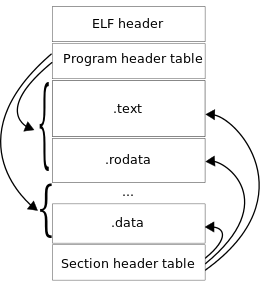
\includegraphics[width=8cm,height=10cm]{images/elf.png}
    \end{center}
    一個ELF OBJ檔隨著它存在的時期有不一樣的需求與組成名詞,在要連結linking時期
    躺在硬碟,包含了
    \begin{verbatim}
ELF header
program header table (可以不要)
section 0
section 1
section 2
section 3
section ...
section n
section header table
    \end{verbatim}
    ELF header 放了ELF所定義的一些例如ELF格式識別字串(俗稱magic number)
    ,還有是那種OBJ檔案type(shared obj, relocatable還是executable)等等
    這種general的資訊。
    \\\\
    program header table描述了一個segment的資訊,segment跟section不太一樣是屬
    於程式執行期的元素,所以在程式執行時期是必要的, 在連結時期是不必要的,
    所以如果你的程式不做連結動作只要有program table就好,
    \\\\
    section header table就是一個索引表來記錄各個section的索引
    \\\\
    sections就是把需要的資料根據屬性用途分門別類後的小集合,
    有.bss .data .init .debug .dynamic .fini .text ........,
    其中比較重要的
    \begin{description}%[align=right]
      \item [.fini] 裡面藏著finish的code,正常exit的code。
      \item [.init] 裡面藏著起始的code,也就是main開始的地方。
      \item [.text] 裡面就是真的CPU指令
      \item [*COM*] common section,只存在relocate object檔中,放沒有init的全域變數與extern 變數。
      \item [.bss] 在relocate object檔中,放有init的全域變數,在executable檔中,放沒有initialize的全域變數。
      \item [.data] 放有initialize的data
      \item [.debug] 放有可以讓gdb trace程式的資訊
      \item [.dynamic] 動態shared object的資訊
    \end{description}
    .bss, *COM*跟.data是一般比較混淆的地方,跟relocate, executable兩種檔案有關,
    要小心。 3 informations比較常用到
    \begin{itemize}
      \item symbol table 關於所有變數函式的參照table
      \item debug info 能讓gdb使用來trace的debug資訊。
      \item dynamic symbol table 給shared obj連結的資訊。
    \end{itemize}
    我們用小程式來看各 section 的儲存資料。
    \begin{verbatim}
#include <stdio.h>
#include <stdlib.h>

int global_a;
char global_b = 5;
static int global_c;
static char global_d = 5;
char *global_str0 = "string0";
char global_str1[] = "string1";
char global_array[3] = {1, 2, 3};

int func()
{
        int func_a;
}

int main()
{
        int main_a;
        char main_b = 15;
        static int main_c;
        static char main_d = 5;
        char *main_str0 = "str0";
        char main_str1[] = "str1";
        char main_array[3] = {1, 2, 3};
        int global_a;
        int *heap_a;

        heap_a = (int *) malloc(sizeof(int) * 4);
}
  \end{verbatim}
  用gcc -g mysection.c 編譯完後,使用objdump -x a.out 可以看出所有的header內容。
  可以看出來gcc對"執行檔"的設計是只有static 與 glboal 變數放在 .data .bss,有
  給值的放在.data,沒給值的放在.bss,全域func放在 .text 。.data裏面還可分可變
  read write 與不可變 read only 的變數。另外在relocate檔中的全域init與非init變數
  還有extern變數放的地方跟executable檔不太一樣。
  \begin{verbatim}

a.out:     file format elf64-x86-64
a.out
architecture: i386:x86-64, flags 0x00000112:
EXEC_P, HAS_SYMS, D_PAGED
start address 0x0000000000400410

Program Header:
    PHDR off    0x0000000000000040 vaddr 0x0000000000400040 paddr 0x0000000000400040 align 2**3
         filesz 0x00000000000001c0 memsz 0x00000000000001c0 flags r-x
  INTERP off    0x0000000000000200 vaddr 0x0000000000400200 paddr 0x0000000000400200 align 2**0
         filesz 0x000000000000001c memsz 0x000000000000001c flags r--
    LOAD off    0x0000000000000000 vaddr 0x0000000000400000 paddr 0x0000000000400000 align 2**21
         filesz 0x0000000000000734 memsz 0x0000000000000734 flags r-x
    LOAD off    0x0000000000000738 vaddr 0x0000000000600738 paddr 0x0000000000600738 align 2**21
         filesz 0x000000000000024c memsz 0x0000000000000260 flags rw-
 DYNAMIC off    0x0000000000000750 vaddr 0x0000000000600750 paddr 0x0000000000600750 align 2**3
         filesz 0x00000000000001d0 memsz 0x00000000000001d0 flags rw-
    NOTE off    0x000000000000021c vaddr 0x000000000040021c paddr 0x000000000040021c align 2**2
         filesz 0x0000000000000044 memsz 0x0000000000000044 flags r--
EH_FRAME off    0x00000000000005e4 vaddr 0x00000000004005e4 paddr 0x00000000004005e4 align 2**2
         filesz 0x000000000000003c memsz 0x000000000000003c flags r--
   STACK off    0x0000000000000000 vaddr 0x0000000000000000 paddr 0x0000000000000000 align 2**4
         filesz 0x0000000000000000 memsz 0x0000000000000000 flags rw-

Dynamic Section:
  NEEDED               libc.so.6
  INIT                 0x00000000004003a8
  FINI                 0x00000000004005c4
  INIT_ARRAY           0x0000000000600738
  INIT_ARRAYSZ         0x0000000000000008
  FINI_ARRAY           0x0000000000600740
  FINI_ARRAYSZ         0x0000000000000008
  GNU_HASH             0x0000000000400260
  STRTAB               0x00000000004002e0
  SYMTAB               0x0000000000400280
  STRSZ                0x000000000000003f
  SYMENT               0x0000000000000018
  DEBUG                0x0000000000000000
  PLTGOT               0x0000000000600928
  PLTRELSZ             0x0000000000000048
  PLTREL               0x0000000000000007
  JMPREL               0x0000000000400360
  RELA                 0x0000000000400348
  RELASZ               0x0000000000000018
  RELAENT              0x0000000000000018
  VERNEED              0x0000000000400328
  VERNEEDNUM           0x0000000000000001
  VERSYM               0x0000000000400320

Version References:
  required from libc.so.6:
    0x09691a75 0x00 02 GLIBC_2.2.5

Sections:
Idx Name          Size      VMA               LMA               File off  Algn
  0 .interp       0000001c  0000000000400200  0000000000400200  00000200  2**0
                  CONTENTS, ALLOC, LOAD, READONLY, DATA
  1 .note.ABI-tag 00000020  000000000040021c  000000000040021c  0000021c  2**2
                  CONTENTS, ALLOC, LOAD, READONLY, DATA
  2 .note.gnu.build-id 00000024  000000000040023c  000000000040023c  0000023c  2**2
                  CONTENTS, ALLOC, LOAD, READONLY, DATA
  3 .gnu.hash     0000001c  0000000000400260  0000000000400260  00000260  2**3
                  CONTENTS, ALLOC, LOAD, READONLY, DATA
  4 .dynsym       00000060  0000000000400280  0000000000400280  00000280  2**3
                  CONTENTS, ALLOC, LOAD, READONLY, DATA
  5 .dynstr       0000003f  00000000004002e0  00000000004002e0  000002e0  2**0
                  CONTENTS, ALLOC, LOAD, READONLY, DATA
  6 .gnu.version  00000008  0000000000400320  0000000000400320  00000320  2**1
                  CONTENTS, ALLOC, LOAD, READONLY, DATA
  7 .gnu.version_r 00000020  0000000000400328  0000000000400328  00000328  2**3
                  CONTENTS, ALLOC, LOAD, READONLY, DATA
  8 .rela.dyn     00000018  0000000000400348  0000000000400348  00000348  2**3
                  CONTENTS, ALLOC, LOAD, READONLY, DATA
  9 .rela.plt     00000048  0000000000400360  0000000000400360  00000360  2**3
                  CONTENTS, ALLOC, LOAD, READONLY, DATA
 10 .init         0000001a  00000000004003a8  00000000004003a8  000003a8  2**2
                  CONTENTS, ALLOC, LOAD, READONLY, CODE
 11 .plt          00000040  00000000004003d0  00000000004003d0  000003d0  2**4
                  CONTENTS, ALLOC, LOAD, READONLY, CODE
 12 .text         000001b2  0000000000400410  0000000000400410  00000410  2**4
                  CONTENTS, ALLOC, LOAD, READONLY, CODE
 13 .fini         00000009  00000000004005c4  00000000004005c4  000005c4  2**2
                  CONTENTS, ALLOC, LOAD, READONLY, CODE
 14 .rodata       00000011  00000000004005d0  00000000004005d0  000005d0  2**2
                  CONTENTS, ALLOC, LOAD, READONLY, DATA
 15 .eh_frame_hdr 0000003c  00000000004005e4  00000000004005e4  000005e4  2**2
                  CONTENTS, ALLOC, LOAD, READONLY, DATA
 16 .eh_frame     00000114  0000000000400620  0000000000400620  00000620  2**3
                  CONTENTS, ALLOC, LOAD, READONLY, DATA
 17 .init_array   00000008  0000000000600738  0000000000600738  00000738  2**3
                  CONTENTS, ALLOC, LOAD, DATA
 18 .fini_array   00000008  0000000000600740  0000000000600740  00000740  2**3
                  CONTENTS, ALLOC, LOAD, DATA
 19 .jcr          00000008  0000000000600748  0000000000600748  00000748  2**3
                  CONTENTS, ALLOC, LOAD, DATA
 20 .dynamic      000001d0  0000000000600750  0000000000600750  00000750  2**3
                  CONTENTS, ALLOC, LOAD, DATA
 21 .got          00000008  0000000000600920  0000000000600920  00000920  2**3
                  CONTENTS, ALLOC, LOAD, DATA
 22 .got.plt      00000030  0000000000600928  0000000000600928  00000928  2**3
                  CONTENTS, ALLOC, LOAD, DATA
 23 .data         0000002c  0000000000600958  0000000000600958  00000958  2**3
                  CONTENTS, ALLOC, LOAD, DATA
 24 .bss          00000014  0000000000600984  0000000000600984  00000984  2**2
                  ALLOC
 25 .comment      0000003a  0000000000000000  0000000000000000  00000984  2**0
                  CONTENTS, READONLY
 26 .debug_aranges 00000030  0000000000000000  0000000000000000  000009be  2**0
                  CONTENTS, READONLY, DEBUGGING
 27 .debug_info   00000226  0000000000000000  0000000000000000  000009ee  2**0
                  CONTENTS, READONLY, DEBUGGING
 28 .debug_abbrev 000000a6  0000000000000000  0000000000000000  00000c14  2**0
                  CONTENTS, READONLY, DEBUGGING
 29 .debug_line   00000047  0000000000000000  0000000000000000  00000cba  2**0
                  CONTENTS, READONLY, DEBUGGING
 30 .debug_str    0000013a  0000000000000000  0000000000000000  00000d01  2**0
                  CONTENTS, READONLY, DEBUGGING
SYMBOL TABLE:
0000000000400200 l    d  .interp	0000000000000000              .interp
000000000040021c l    d  .note.ABI-tag	0000000000000000              .note.ABI-tag
000000000040023c l    d  .note.gnu.build-id	0000000000000000              .note.gnu.build-id
0000000000400260 l    d  .gnu.hash	0000000000000000              .gnu.hash
0000000000400280 l    d  .dynsym	0000000000000000              .dynsym
00000000004002e0 l    d  .dynstr	0000000000000000              .dynstr
0000000000400320 l    d  .gnu.version	0000000000000000              .gnu.version
0000000000400328 l    d  .gnu.version_r	0000000000000000              .gnu.version_r
0000000000400348 l    d  .rela.dyn	0000000000000000              .rela.dyn
0000000000400360 l    d  .rela.plt	0000000000000000              .rela.plt
00000000004003a8 l    d  .init	0000000000000000              .init
00000000004003d0 l    d  .plt	0000000000000000              .plt
0000000000400410 l    d  .text	0000000000000000              .text
00000000004005c4 l    d  .fini	0000000000000000              .fini
00000000004005d0 l    d  .rodata	0000000000000000              .rodata
00000000004005e4 l    d  .eh_frame_hdr	0000000000000000              .eh_frame_hdr
0000000000400620 l    d  .eh_frame	0000000000000000              .eh_frame
0000000000600738 l    d  .init_array	0000000000000000              .init_array
0000000000600740 l    d  .fini_array	0000000000000000              .fini_array
0000000000600748 l    d  .jcr	0000000000000000              .jcr
0000000000600750 l    d  .dynamic	0000000000000000              .dynamic
0000000000600920 l    d  .got	0000000000000000              .got
0000000000600928 l    d  .got.plt	0000000000000000              .got.plt
0000000000600958 l    d  .data	0000000000000000              .data
0000000000600984 l    d  .bss	0000000000000000              .bss
0000000000000000 l    d  .comment	0000000000000000              .comment
0000000000000000 l    d  .debug_aranges	0000000000000000              .debug_aranges
0000000000000000 l    d  .debug_info	0000000000000000              .debug_info
0000000000000000 l    d  .debug_abbrev	0000000000000000              .debug_abbrev
0000000000000000 l    d  .debug_line	0000000000000000              .debug_line
0000000000000000 l    d  .debug_str	0000000000000000              .debug_str
0000000000000000 l    df *ABS*	0000000000000000              crtstuff.c
0000000000600748 l     O .jcr	0000000000000000              __JCR_LIST__
0000000000400440 l     F .text	0000000000000000              deregister_tm_clones
0000000000400480 l     F .text	0000000000000000              register_tm_clones
00000000004004c0 l     F .text	0000000000000000              __do_global_dtors_aux
0000000000600984 l     O .bss	0000000000000001              completed.6661
0000000000600740 l     O .fini_array	0000000000000000              __do_global_dtors_aux_fini_array_entry
00000000004004e0 l     F .text	0000000000000000              frame_dummy
0000000000600738 l     O .init_array	0000000000000000              __frame_dummy_init_array_entry
0000000000000000 l    df *ABS*	0000000000000000              mysection.c
0000000000600988 l     O .bss	0000000000000004              global_c
0000000000600969 l     O .data	0000000000000001              global_d
0000000000600983 l     O .data	0000000000000001              main_d.2722
000000000060098c l     O .bss	0000000000000004              main_c.2721
0000000000000000 l    df *ABS*	0000000000000000              crtstuff.c
0000000000400730 l     O .eh_frame	0000000000000000              __FRAME_END__
0000000000600748 l     O .jcr	0000000000000000              __JCR_END__
0000000000000000 l    df *ABS*	0000000000000000              
0000000000600740 l       .init_array	0000000000000000              __init_array_end
0000000000600750 l     O .dynamic	0000000000000000              _DYNAMIC
0000000000600738 l       .init_array	0000000000000000              __init_array_start
0000000000600928 l     O .got.plt	0000000000000000              _GLOBAL_OFFSET_TABLE_
00000000004005c0 g     F .text	0000000000000002              __libc_csu_fini
0000000000600968 g     O .data	0000000000000001              global_b
0000000000000000  w      *UND*	0000000000000000              _ITM_deregisterTMCloneTable
0000000000600958  w      .data	0000000000000000              data_start
0000000000600990 g     O .bss	0000000000000004              global_a
0000000000600984 g       .data	0000000000000000              _edata
00000000004005c4 g     F .fini	0000000000000000              _fini
0000000000600978 g     O .data	0000000000000008              global_str1
0000000000000000       F *UND*	0000000000000000              __libc_start_main@@GLIBC_2.2.5
0000000000600958 g       .data	0000000000000000              __data_start
0000000000000000  w      *UND*	0000000000000000              __gmon_start__
0000000000600960 g     O .data	0000000000000000              .hidden __dso_handle
00000000004005d0 g     O .rodata	0000000000000004              _IO_stdin_used
0000000000400506 g     F .text	0000000000000006              func
0000000000400550 g     F .text	0000000000000065              __libc_csu_init
0000000000000000       F *UND*	0000000000000000              malloc@@GLIBC_2.2.5
0000000000600998 g       .bss	0000000000000000              _end
0000000000400410 g     F .text	0000000000000000              _start
0000000000600984 g       .bss	0000000000000000              __bss_start
000000000040050c g     F .text	000000000000003b              main
0000000000000000  w      *UND*	0000000000000000              _Jv_RegisterClasses
0000000000600970 g     O .data	0000000000000008              global_str0
0000000000600988 g     O .data	0000000000000000              .hidden __TMC_END__
0000000000000000  w      *UND*	0000000000000000              _ITM_registerTMCloneTable
00000000004003a8 g     F .init	0000000000000000              _init
0000000000600980 g     O .data	0000000000000003              global_array
  \end{verbatim}
  當呼叫一個程式時,exec系統呼叫會跳去OS loader的code執行,在linux的實作中,
  executable裏面會藏有一個linker stub code,會去load真正dynamic linker,
  最後從一個\_start這個函式開始而不是main開始,\_start後來會去叫
  main,所以如果要精簡的話,就不要用gcc編譯直接寫組語用\_start就好了。
  另外像section header table如果你不需要做連結動作這也可以拿掉,
  還有可執行檔的symbol table等,我們其實可以把這些全部拿掉,不過這要用組語並且
  用nasm來建造我們的執行檔。其實還有很多東西,這就是為什麼即使我們根本就沒呼叫
  任何函數,用C做成的動態檔,用ldd看一定有ld-linux.so libc.so了。
  \\\\
  完整的elf規格可以在
  \href{http://en.wikipedia.org/wiki/Executable_and_Linkable_Format}{這裡找到}
  ,或更\href{http://www.akkadia.org/drepper/dsohowto.pdf}{深入的介紹}。

    \subsection{常用工具}
    \begin{description}
      \item [as] 組譯器assembler
      \item [ld] 連結器link editor 同時也是建造shared obj(libxxx.so)的建造。
      \item [nm] 列出這個obj檔的symbol table。
      \item [objdump] 列出obj檔的資訊
      \item [readelf] 專讀elf格式obj檔,並印出相關資訊。
      \item [strings] 看string table,只是看這個檔裡面有什麼秀的出來的文字。
           string在ELF格式裡面用來代表symbol與section的名字。
      \item [strip] 刪除不必要的obj檔裏面資訊,例如symbol table還有debug stab
          這樣的OBJ檔無法用nm看出symbol, 也無法用gdb來除錯了。
      \item [ar] 捆綁obj檔案,類似tar。 archive(靜態連結函數庫libxxx.a)的建造,
        這也是debian package deb的捆綁格式。
      \item [ranlib] 建造lib檔的index命令。
      \item [objcopy] 修改obj檔後,copy修改過的資料成一個新obj檔。
      \item [gprof] 測試程式執行時間,以及了解function彼此呼叫的關係稱為profiling
    \end{description}
    binutils裏面很重要的是有library能讀懂各式obj檔案格式的library,稱BDF library
    (binary file descriptor library),就好像有個影像library能讀懂gif, jpg, png
    ...等不同格式,當然在Linux上最重要的就是elf格式。as, ld 跟 objdump 都是使用
    binutils裏面的 BFD 去讀取elf的資訊,但其中readelf是直接讀obj檔案
    出來,自己去解釋elf資訊,這是另一個工具去驗證BFD到底對不對,而且本身也提供
    比 BFD 更多elf資訊的小工具。 BFD 有很多功能function 例如endian byte order,
    architecture, relocation計算等等,都是在BFD裏面實作。
    \\\\
    binutils裏面的工具可以讀懂這些elf格式檔也能做出一些對section的增加刪除
    的動作處理。
    \begin{verbatim}
nm -a a.out 顯示所有symbol資訊
nm -d a.out 顯示dynamic section symbol資訊
readelf -a a.out 顯示所有資訊
objdump -x a.out 顯示所有資訊
objdump -W a.out 顯示DWAFR資訊 
objdump -G a.out 顯示STAB資訊
objdump -D a.out 反組譯
strip a.out --strip-debug --strip-unneeded
    \end{verbatim}
    其中比較不一樣的是gcc 加上-g會加上debug的資訊,這資訊也有兩種格式,分為
    STAB與DWARF兩種,有關的操作在objdump 裏面。而這debug資訊往往只對開發人員有
    用,在ship給客戶的執行檔中是要拿掉的以減少硬體資源,但出錯時卻又要拿回來
    除錯,所以必須把每次release的image跟除錯 debug object管理好,等將來gdb
    可以拿回來使用。使用objcopy可以拿出我們想要的section
    \begin{verbatim}
把a.out的debug info留下存成a.out.debug
objcopy --only-keep-debug a.out a.out.debug

把a.out.debug的debuglink指向a.out
objcopy --add-gnu-debuglink a.out.debug a.out
    \end{verbatim}
    則如此當a.out出問題時,我們可以光拿到core,用gdb就可以把debug symbol拿回來
    並且backtrace看死在哪裡。這請看debug的章節有更多例子。

  \section{libtool}
  在前面的實驗中,我們建立了static lib需要的.o也建造了dyanmic lib需要的PIC .o
  ,如果這project支援多種類*nix, 像AIX, Linux, HP-UX....則是很麻煩的需要了解各系
  統的底層,libtool是GNU的跨平台library建造工具介面,利用libtool就可以很快建立
  相對應的library。libtool有很多種mode,就是分別對應gcc的動作, compile, link
  , install等等。不同mode
  \begin{verbatim}
  libtool --mode=compile gcc -c test.c
  libtool --mode=link gcc -g -o libtest.la test.lo -rpath /tmp
  \end{verbatim}
  最基本的就是compile與link兩個,compile會自動產生3個檔案
  \begin{itemize}
    \item .libs/test.o shared object, 編譯test.c用上-fPIC -DPIC
    \item test.o normal object,將來可以做成static lib的
    \item test.lo 是個文字檔, 多出來記載上面兩種object的位置。將來libtool
      link時都要用這個假的object檔來工作。
  \end{itemize}
  所以lo檔是將來要pass給libtool的假object檔。rpath跟link的那個rpath一樣,
  是會寫進so檔去有關rpath的資訊。而且要加這選項才會產生.so檔。
  \\\\
  mode=link會產生
  \begin{itemize}
    \item .libs/libtest.so.0.0.0
    \item .libs/libtest.a
    \item libtest.la
  \end{itemize}
  這樣看很清楚了,跟lo檔一樣意思,la檔是將來連結執行檔時會使用的。我們必須先
  把這些東西都裝到暫存區,符合當初rpath指定目錄。
  \begin{verbatim}
  libtool --mode=install install -c libtest.la /tmp
  用finish會做ldconfig 加到cache去,可以不用做這個
  libtool --mode=finish /tmp
  \end{verbatim}
  所以我們寫個main.c,裏面有int main( ... )的程式。
  \begin{verbatim}
$ libtool --mode=compile gcc -c main.c
$ libtool --mode=link gcc -o main.dynamic main.lo /tmp/libtest.la
$ libtool --mode=link gcc -o main.static main.lo /tmp/libtest.la -static-libtool-libs
  \end{verbatim}
  會產生shared跟static的main.dynamic 與 main.static,也可以直接
  \begin{verbatim}
$ libtool --mode=compile gcc -c main.c
$ libtool --mode=link gcc -o main.dynamic main.lo libtest.la
  \end{verbatim}
  但是這個main.dynamic 不是shared的執行檔,只是shell script,所以必須用execute
  mode來執行gdb。
  \begin{verbatim}
$ libtool --mode=execute gdb main.dynamic
  \end{verbatim}
  我們常看到有些project的結果是shell script,就是用這種方法建立的。

  \section{profiling}
    程式寫的好不好有很多判斷標準,有一個是performance的標準,profiling要
    gcc編譯時多加-pg選項才會把一些資訊寫進去。
    \begin{verbatim}
    $ gcc -pg -g my.cc
    \end{verbatim}
    產生的a.out,要先執行一次,會產生gmon.out這個profiling所需的檔案。
    就可以拿a.out跟gmon.out來分析程式performance
    \begin{verbatim}
    $ gprof a.out gmon.out > analysis.txt
    \end{verbatim}
    這analysis.txt分成兩大部份
    \begin{itemize}
      \item flat profile 單純每個function執行的時間
      \item call graph 包含呼叫子function的所有時間,所以main應該是100%
    \end{itemize}

    \begin{verbatim}
Flat profile:

Each sample counts as 0.01 seconds.
%   cumulative   self              self     total           
time   seconds   seconds    calls   s/call   s/call  name    
50.55      9.09     9.09        1     9.09     9.09  func2
50.55     18.19     9.09        1     9.09     9.09  func1
 0.17     18.22     0.03                             main

                     Call graph (explanation follows)


granularity: each sample hit covers 2 byte(s) for 0.05% of 18.22 seconds

index % time    self  children    called     name
                                                 <spontaneous>
[1]    100.0    0.03   18.19                 main [1]
                9.09    0.00       1/1           func2 [2]
                9.09    0.00       1/1           func1 [3]
-----------------------------------------------
                9.09    0.00       1/1           main [1]
[2]     49.9    9.09    0.00       1         func2 [2]
-----------------------------------------------
                9.09    0.00       1/1           main [1]
[3]     49.9    9.09    0.00       1         func1 [3]
-----------------------------------------------

    \end{verbatim}
    其他選項
    \begin{itemize}
      \item gprof -a 不顯示static function
      \item gprof -b 不顯示說明書
      \item gprof -pfunc1 -b 只顯示func1與不顯示說明書
    \end{itemize}
  \section{結語}
  所以其實整個系統很簡單,就是一堆函式庫,各個應用程式呼叫這些已經編好
  的函式庫,因此只要有函式庫,就可以跑想要的程式,所以在GNOME這個桌
  面環境下,也可以跑用Qt這個函式庫寫出來的程式,也可以跑Motif這個函式庫
  的程式。Linux上的程式就是讀文字設定檔,做完設定呼叫函式庫,完成一件工
  作,就這麼簡單。
  \\\\
  除了gcc外,目前還有一個clang是由apple開發並opensource的C編譯器frontend,他的
  編譯引擎是由 University of Illinois at Urbana–Champaign 所做的llvm,
  他是由c++所完成,在很多評比上比gcc要好,也促使GNU小組的思考與轉換嘗試。

  \chapter{project與build管理}
我們在前面編譯test.c test1.c 時,發現有很多動作是很重複的,或者整個大 project
的c cc檔案很多時,編譯過的不想再重編,只想編譯有修改過的c檔,或者編譯時需要
其他東西配合的相依管理等等。傳統上用 Makefile 做這些,而unix like 的系統彼此
之間的差異性與相依性在 opensource 中靠 autotools 幫我們處理。
\\\\
java 的世界可能用ant, maven,但那語法就是xml語法與他的tag了。現在還多了個
gradle ,ant 可能是那些不習慣奇怪變數的人發明的,maven 比 ant 好是多了相關
library 的相依性紀錄與下載,gradle 就是還多了groovy 的 script,這些東西其實
就是差不多那樣, 也沒什麼好不好的,就跟svn/git一樣,code 寫的亂七八糟,用什
麼工具都沒用。 不過make可以用熟悉的 shell script, 所以我還是喜歡 make 多一點。

\section{Makefile}
寫程式寫很大時,我們會分成好幾個模組,就是一個個的C或其他程式語言的
小檔案。make是編譯大量的 source code 一定要用到的工具,最常用的就是寫一個
Makefile,他會根據這裡面的目標(target)所定義的規則(rule)來做編譯的
動作,並創造出可執行的程式來。一般人都會說拿到 source code 不知從何
讀起,其實除了 README 等文件外,Makdefile 是最能知道程式流程的檔案,
你可以看 Makefile 然後找到程式的入口檔案,一步步追下去,用我們在
編輯器講到的方法來追程式。不過現在 Makefile 越寫越專業越來越大也
不太容易看懂。
\\\\
一個 Makefile 其實只是一堆的規則(rule)所組成。一個規則的型式是這樣的
target:prequiste ; command(新文件變成recipe) 通常是寫成
\begin{verbatim} 
target: prerequiste
	command
	command
	command
\end{verbatim} 
如果一行不夠寫要分兩行,可以用\verb=\=來變成兩行底下是一個簡單 Makefile 例子
\begin{verbatim}
SHELL=/usr/bin/bash

edit:	main.o kbd.o command.o display.o \
        insert.o search.o files.o utils.o
        $(CC) -o edit main.o kbd.o command.o display.o \
        insert.o search.o files.o utils.o
      
command.o : command.c command.h
        $(CC) -o command.o command.c

clean:
        @rm *.o *~
\end{verbatim}
其中定義了 SHELL 這個變數,表示用/usr/bin/bash來解釋shell執行。
有3個目標 (target) : edit command.o 與clean,
雖然沒有定義CC這個變數,用了內定變數\$(CC)去編譯程式。
如果給
\begin{verbatim}
$ make clean
\end{verbatim}
make會另外叫起一個shell來執行 command 這裡面的字串也就是rm *.o。如果給
\begin{verbatim}
$ make edit
\end{verbatim}
make會去檢查需要的先決條件(prerequiste)發現有個檔名target command.o 
存在,會依序根據規則來編譯。rebuild時,會根據target與prerequiste的
timestamp 決定要不要重新rebuild,如果沒有這檔案,或者有新c檔案等,
就會重新編譯,不然就只是編譯prerequiste檔的timestamp比較新的檔。當然也可以
touch directory或使用永遠編譯的選項。
  \subsection{變數(variables)}
  像寫程式一樣,make規則裡面的組成可以有動態的值,這時就需要用變數來
  設值來取代與轉換以及日後維護。另外還有就是有時字太多了,打字打到
  可能會出錯,這樣除錯起Makefile很不好除錯,用變數代換值可以減少一
  些打字錯誤。變數也有一些規定,
  \begin{itemize}
    \item 字母大小有差。不要用字母數字底線以外的字元。可以有空格在前面後面。
          (像shell script就不行有空格在變數前後。Var = value跟Var=value
          是不一樣的)。
    \item 使用變數用\$(VAR)或者\${VAR}都可以。
    \item 如果要用\$,請多加一個\$變成\$\$,在Shell Command會用到Shell
          變數此時就要加\$。
          \begin{verbatim}
linuxsubdirs: dummy
	  set -e; for i in $(Subdirs); do $(MAKE) -C $$i; done
          \end{verbatim}
    \item 變數代換有兩種很重要的不同代換。遞迴的變數代換 var  = value 
	  (recursively expand)只要變數的值又是另一個變數值時,
	  就會一直代換下去。簡單的變數代換(simple expand) var := value 
          只代換一次變數的值。傳統的Makefile是沒有var :=的,這是GNU 的
          \begin{verbatim}
	  例子
foo = $(bar)
bar = $(ugh)
ugh = Huh?
	      
all:
	echo $(foo)
	  會echo Huh?
          \end{verbatim}
          ,遞迴的方法有個壞處,不能夠加東西上去,例如
          \begin{verbatim}
CFLAGS = -Isrc/include
CFLAGS = $(CFLAGS) -O
          \end{verbatim}
	  則會一直玩不完,就慘了,這可以用
          \begin{verbatim}
CFLAGS := $(CFLAGS) -O
或
CFLAGS += -O
          \end{verbatim}
          兩種方法解決,其中 := 又可以寫成 ::= ,這是新的posix 2012定義。
    \item shell與Makefile變數
	  wildcard在shell變數中可以展成所有的意義,但是在Makefile中使用要小心,
          例如
          \begin{verbatim}
OBJECTS = *.o
foo: $(OBJECTS)
	cc -o foo $(OBJECTS)
          \end{verbatim}
          如果目前目錄下有.o檔,會自動展開這些.o檔作 target,如果目前目錄下面
          沒有.o檔,則wildcard展不開,make並不知道你要的target是那些.o檔,
	  他以為要去找一個叫*.o的target,這時就會跟你說找不到。但由於implicit
          rule(內隱規則)中,Makefile會自動去找x.o的生成時,會自動找x.c x.s ...
          等檔案, 會用內隱規則 \verb=$(CC) $(CPPFLAGS) $(CFLAGS) -c -o $@ $<=
          去編譯,結果就變成 \verb=$(CC) $(CPPFLAGS) $(CFLAGS) -c -o '*.o' *.c=
          ,但由於 \$< 只是第一個所有先決條件,所以就是 wildcard 還回來的第一個
          .c 檔案被編譯而已,因此 OBJECTS 要設成 prog1.o prog2.o 這樣的形式比
          較好。 另外每一行 command 其實是喚起一個 sub shell 來執行所以*.o會被
          shell, bash 解讀而沒有問題。
	  cc -o foo \$(OBJECTS) 的 \$(OBJECTS) 是可以展成所有的.o檔的。
	
    \item 變數給Shell可以用
          \begin{verbatim}
export var1 var2 var3....
          \end{verbatim}
	  而想要把shell變數的值傳給Makefile變數有兩個情況,
	  一個是原本的環境變數自動會變成同樣的Makefile變數名,
	  可以直接使用。如果兩個有相同的變數名,用make -e 則
	  Shell的會蓋掉Makefile裡的定義。
	  另一個狀況是想要根據一個shell的執行傳回的字串來設變數,
	  這時需要用內建函式,\$(shell shell\_command)
          \begin{verbatim}
VAR := $(shell shell_command)
          \end{verbatim}
    \item 特定Target的變數
	  例如
          \begin{verbatim}
prog : CFLAGS = -g
prog : prog.o foo.o bar.o
          \end{verbatim}
	  當要編譯 prog 這個target時,才設CFLAGS為`-g',同時當要編譯
	  prog.o foo.o,bar.o時也會同時設CFLAGS=-g,這是因為某種設定只為了
	  某個特定的target才須要,例如程式除錯時就很有用。
  \end{itemize}

  \subsection{target}
  目標可以是檔名或者是一個代表動作的識別符號,如果不是檔名的Target叫 phony 
  target。make根據指定的target來做相關動作。要完成一個目標前會先檢查他所需
  要的檔案或要先做的phnoy target,即相依性檔案或先決條件目標 (dependency 
  or prerequiste) 如果要的相依或先決目標不存在,則make會失敗。如果這裡的先決
  目標是 phony target 則 PHONY TARGET 每次都會被執行。
  \\\\
  如果你在 shell prompt 只下 make 命令而已,第一個 rule 永遠被執行。這叫
  default goal。如果你有指定target名字,例如make clean,則會去執行這個
  target的動作,以上面例子看就是會執行 rm *.o *~ 這個動作。
  \\\\
  \subsubsection{一些目標規定}
  有些phony目標是GNU建議的,不見得一定要有啦只是建議目標。例如
  \begin{itemize}
    \item all           :內定的編譯動作
    \item install       :安裝binary檔的動作
    \item clean         :清除obj檔的動作
    \item dist          :產生configure的動作
    \item distclean	:清除configure所產生的檔
  \end{itemize}
  有的像clobber,這個也常出現在phony target中,表示剷了再除,除了在剷徹底剷除。
  \subsubsection{特別的內定目標(built-in target)}
  有些是已經有特殊意義的target,比較常用的
  \begin{itemize}
    \item .PHONY 在這個後面的target無條件執行。因為例如
      \begin{verbatim}
clean:
         rm *.o
      \end{verbatim}
      如果萬一真的有一個叫clean的檔案在make的目錄下,偏偏這個檔沒有update,日期
      沒變,所以當你make clean時,make認為這個clean已經有了,也沒有相依性檔案需
      要重新編譯,於是就不執行rm *.o了 。 所以我們要把它寫在.PHONY,則每次make
      clean就無條件執行,不會把clean看成是檔名。
    \item .SUFFIX 副檔名內定編譯名單。make有一些內定方法編譯特別副檔名,這些
      副檔名規則的副檔名 (名單)list,是在SUFFIXS這個變數裡,可能有.c .o .cpp
      等等。用
      \begin{verbatim}
.SUFFIXS:
      \end{verbatim}
      清掉名單,或用
      \begin{verbatim}
.SUFFIXS: .sgml .hack  
      \end{verbatim}
      加到名單去,則在用內隱規則的suffix rule時,會自動引用。
    \item .SILENT 這裡面的target執行時 命令(command)將不會印出來
    \item .EXPORT\_ALL\_VARIABLES 把所有變數告訴後來sub shell的子程序
  \end{itemize}

  \subsection{command}
  命令就是要完成一個目標所要做的動作,有幾個比較重要的規定要清楚
  \begin{itemize}
    \item command 前面一定要是個TAB鍵。不可以用空白鍵。
    \item 每一行的命令其實都是喚起一個sub shell來執行命令,做完了,
          這個sub shell就沒有了。
    \item 所以更改過的變化不能傳給下一行命令。如果要把執行結果傳給下一
          行必須寫在同一行裡。例如
          \begin{verbatim}     
cd editor
$(MAKE) all
          \end{verbatim}     
          這樣cd到editor目錄的結果並沒有傳給下一個make all的這個shell。
          必須這樣寫
          \begin{verbatim}     
cd editor; \
$(MAKE) all
          \end{verbatim}     
          所以如果有if, while等等判斷在shell內,就必須寫成一行,
          或用\verb=\=來分成很多行。
    \item 要把錯誤掠過不看在命令前加個-,
          要不秀出命令在螢幕上加個@,例如前面例子裡的clean這個target。
    \item 喚起的sub shell要用什麼shell,是定義在SHELL這個變數裡。
  \end{itemize}

  \subsection{內隱規則(Implicit Rules)}
  implicit rules的使用是Makefile最重要的部份,也是一般人剛接
  觸摸不著邊的問題所在。裏面有很多看不到的自動使用要清楚。
  通常我們編譯程式時有很多算是每個人都有的共同習慣,例如我就是把
  foo.c 編成foo.o。像這樣的編譯習慣,gnu make有一些內定規則來編譯,
  也就是有的target你不寫,make也可以根據內定規則把他編譯出來。不用
  對每個不同的.o寫不同的規則,
  如果有個程式由foo.c foo1.c foo2.c......寫這些就寫得會發瘋了,例如
  \begin{verbatim}
foo.o:foo.c
        gcc -c -o foo.o foo.c
foo1.o:foo1.c
        gcc -c -o foo1.o foo1.c
....
  \end{verbatim}
  因此如果你不寫foo.o的規則,那麼make當別的規則用到foo.o時,他找不到規則
  來編,就會自動找foo.c來編譯。這樣看不到的編譯規則有很多,如
  \begin{verbatim}
$(CC) -c $(CPPFLAGS) $(CFLAGS) xxx.c來編譯
  \end{verbatim}
  或者找不到.c時會去找.cc, .cpp, .C檔
  \begin{verbatim}

C++程式產生 xxx.o
$(CXX) -c $(CPPFLAGS) xxx.cpp

TeX 產生 xxx.dvi
$(TEX) xxx.tex

Pascal 產生xxx.o
$(PC) -c $(PFLAGS) xxx.p

  \end{verbatim}
  如果是單一檔名例如foo為target,則是會先自動找foo.o,自動使用
  LDFLAGS, LOADLIBES, LDLIBS 這3個變數
  \begin{verbatim}

$(CC) $(LDFLAGS) foo.o $(LOADLIBES) $(LDLIBS)

  \end{verbatim}
  \subsubsection{自己的內隱規則}
  因為可能有的時候你希望做些dependency檢查,或者加上一些gcc
  用的旗標,不是很單純的編譯而已你可以給make自訂的內隱規則,
  自訂規則通常有兩種常用,pattern rule與suffix rule.
  \\\\
  樣式規則(pattern rule)使用百分比符號代表一個 pattern,
  你可以用pattern rule來做一些自定的內隱規則。像這樣
  \begin{verbatim}
%.o : %.c prog.h
	$(CC) $(CFLAGS) $(DEBUG_FLAG) -c -o $@ $<
  \end{verbatim}
  或者
  \begin{verbatim}
%.pdf : %.sgml
	db2pdf $<
  \end{verbatim}
  \%表示所有相對於後面先決條件的檔名的意思,他不是*,因為他
  有一對一的相對應關係,foo.o 就要找foo.c,foo1.o就要找foo1.c,
  所以他不是*。所以上面的意思是所有碰到要.o的target時,去找相
  對應的.c檔,並根據先決條件prog.h做檢查,如果找不到prog.h就不
  做下去了。\%不只可以表現主檔名,其實可以表現任一個相對應的字串,
  所以叫pattern,你可以用s.\%.c,不只用\&.c,其中對應到\%的子字
  串叫stem。另外\$@ \$<...這種符號,叫自動變數,
  \\\\
  pattern rule也可以有特定變數設值,特定樣式(pattern)的變數,例如
  \begin{verbatim}
%.o : CFLAGS = -O
  \end{verbatim}
  表示只要有要編譯xxxx.o的規則時,通通要設CFLAGS為-O。
  \\\\
  副檔名規則(suffix rule) 是比較古老的一種,但他是內定內隱規則的 rule,
  例如前面編譯 .o 的內隱規則,其實是
  \begin{verbatim}
.c.o:
        $(CC) $(CPPFLAGS) $(CFLAGS) -c -o $@ $<
  \end{verbatim}
  很多老Makefile也都用這種rule, 這種方法就有限制性,因為只能用在副檔名的規
  則。例如
  \begin{verbatim}
.c.o:
        $(CC) -c -o $*.o $<
.S.o:
        $(CC) -c -o $*.o $<
  \end{verbatim}
  小心,跟pattern rule的 \%o : \%c順序不一樣喔
  \\\\    
  因為這樣動態的編譯手法,它需要代替一些動態改變的字串。所以有所謂的自動變數
  \begin{itemize}
    \item \$@   同一個規則的目標名
    \item \$*   這個只有在內隱規則中有用。表示樣式或副檔名規則中對應到的字串。
      就是stem
    \item \verb=$<=   同一規則的第一個先決條件名,這個大部分用在suffix rule,因為
	suffix rule只有一個檔。
    \item \$?   同一個規則的所有先決條件名,但是只有原始程式碼改過的比obj檔新
      才會符合,也就是比target還新的先決條件檔案。
    \item \verb=$^=   所有先決條件,但是有的make像solaris make可能不認得這個自
      動變數。
  \end{itemize}
  上面是比較常用的,比較常用還是\verb=$< $@ $*=這3個。內隱規則內也預設了一些編譯變
  數,例如
  \begin{verbatim}
AR = ar
AS = as
CC = cc
MAKE = make
CXX = g++
CPP = $(CC) -E
FC = f77
PC = pc
...
...
ARFLAGS = rv
CFLAGS =
CXXFLAGS =
CPPFLAGS =
LDFLAGS =
FFLAGS =
PFLAGS =
  \end{verbatim}
  當有內隱規則被編譯時,如果什麼都沒有寫他會根據副檔名叫用特別的預設變數
  的compiler,像\$(FC)是fortran 77, \$(AS)是assembly外,當有.c檔案需要編譯
  時除了直接拿\$(CC)來用,還會使用\$(CFLAGS)來當作\$(CC)的compile參數。
  \$(LDFLAGS)當作link時的參數。如果你沒有設CC這個變數,則自動是cc這個值,
  可以直接拿\$(CC)來用。所以光設定CFLAGS跟LDFLAGS完全不用寫怎麼compile .c
  檔案,只要是使用內隱規則的,他也會自動的編譯.c檔案。自定內隱規則可以寫在任
  何地方,make會自動先找到他們,等到要用時就會去用。
  \\\\
  例如有個mk.c
  \begin{verbatim}
$ echo -ne '#include <stdio.h>\nint main() { printf("Hello World\\n"); }' > mk.c
$ cc mk.c -o mk
\end{verbatim}
當make mk時,就會自己找mk.c來編譯,什麼都不需要寫,連Makefile都不用寫

  \subsection{內建函數}
  GNU make有一些內建函式讓我們處理上方便些,函式呼叫的格式是
  \begin{verbatim}
$(function arguments)
  \end{verbatim}
  例如
  \begin{verbatim}
$(subst from,to,text)
$(patsubst %.o,%.c,$(objects))
$(suffix src/foo.c src-1.0/bar.c hacks)
$(dir mydir0/mydir1/myfile)
$(notdir mydir0/mydir1/myfile)
$(wildcard *.c)
$(error err_msg)
files := $(shell echo *.c)
  \end{verbatim}
  可以用subst, patsubst做pattern代換,也可用dir, notdir做類似dirname,basename
  處理。另外由於單純使用*.o, *.xxx有解釋上的問題,所以用 wildcard 得到真正的所
  有名字回來處理。suffix 是用來擷取副檔名用的,任何句點 . 後面的字串會還回來,
  所以例子裏面會還回 .c .c 而已。error則會印出error message後死掉。 常用的最後
  一個,把shell執行結果傳回Makefile做進一步處理,有了 shell 我們可以為所欲為了。
  shell 裡面同樣用變數要兩個\$,可以跨行,但也要用反斜線變一行,跟用 command
  的規定一樣。
  \\\\
  比較常用的字串檔名代換的函數有
  \begin{verbatim}
$(dir src/foo.c pkgs/rpm/rpm.spec) 產生 src pkgs/rpm
$(notdir src/foo.c pkgs/rpm/rpm.spec) 產生 foo.c rpm.spec
$(basename src/foo.c src-1.0/bar hacks) 產生 src/foo src-1.0/bar hacks
$(suffix src/foo.c src-1.0/bar.c) 產生 .c .c
$(addsuffix .c,foo bar) 產生 foo.c bar.c
$(addprefix src/,foo bar) src/foo src/bar
$(wildcard *.c)
$(realpath ./mydoc) 產生真的絕對路徑名
  \end{verbatim}
  字串處理,這跟 shell 的字串處理能力很像,但要注意的是多了 Makefile pattern
  rules 的 \% 處理。
  \begin{verbatim}
$(subst ee,EE,feet on the street) 代換 ee 變成 EE
$(strip " a b c d   ") 去掉前後的空白
$(findstring gyoza,gyoza good good eat) 找 gyoza 這個字,回傳 true/false
$(sort list) 排序
$(wordlist 2, 3, foo bar baz) 傳回 bar baz
$(firstword foo bar) $(lastword foo bar) 只是像 wordlist 方便的呼叫
  \end{verbatim}
  suffix 與 pattern rule 的字串處理,這很有用
  \begin{verbatim}
$(patsubst %.c,%.o,x.c.c bar.c) 像 pattern rule 的代換,產生 x.c.o bar.o

這有一個變數的簡單語法,包含 suffix rule
$(var:pattern=replacement)
$(var:suffix=replacement)
$(target:%.c=%.o) 把變數 target 的 .c 變成 .o
$(target:.o=.c) 把變數 target 的 .c 變成 .o

$(filter %.c %.s,foo.c bar.c foo.s doc.rst foo.h) 只會傳回 .c .s 的檔案
  \end{verbatim}
  錯誤與 logging 處理
  \begin{verbatim}
$(info info message)
$(warning warning message)
$(error error message we want to print and exit)
  \end{verbatim}
  \subsection{條件編譯與MAKE}
  GNU make 裡面可以有條件判斷後,決定要不要做設變數或make,
  其實主要處理一些makefile內的變數與環境,例如
  \begin{verbatim}
ifeq ($(CC),gcc)
  libs=$(libs_for_gcc)
else ifeq ($(CC),clang)
  libs=$(libs_for_clang)
else
  libs=$(normal_libs)
endif
  \end{verbatim}
  判斷\$(CC)這個內隱規則的變數是不是gcc然後選擇函式庫,
  其中ifeq或者ifneq有四種寫法
  \begin{verbatim}
ifneq (arg1, arg2) 
ifneq 'arg1' 'arg2' 
ifneq "arg1" "arg2" 
ifneq "arg1" 'arg2' 
ifneq 'arg1' "arg2" 
  \end{verbatim}
  除了ifeq, ifneq還有ifdef, ifndef,很像c裡面的前置處理。ifdef ifndef 只會測試
  variable是否有定義,如果要測試空字串必須用\verb=ifeq(,$(var))=。
  但如果需要logical and logical or怎麼辦呢? 這時必須用ifneq 跟 function filter
  來達到
  \begin{verbatim}
  ifneq (, $(filter $(GCC_MINOR),4 5))
  \end{verbatim}
  filter的用法是filter X, A B C ..., 傳回 A B C ...任何符合X pattern 的字串,
  所以上面的意思是 GCC minor 號是4 或是 5的都會讓這個ifneq fail掉。就有或的
  logic在裏面了。另外有 function \verb=(or c1,c2,c3 ...) (and c1,c2,c2 ... )=
  ,c1 c2 c3會依序展開,如果有non-empty string, or會停下回傳那個string,如果
  全是空字串,回傳空字串, and 反過來如果碰到空字串,停下回傳空字串,不然就回傳
  最後那個字串。
  \\\\
  最後這些逗號,空格要小心,這些有的一定要空格有的會變成字串的一部份,所以如果
  出問題時要小心空格的位置。

  \subsection{parallel make與gcc dependancy檔}
  當編譯很大時,有些不相關的jobs 可以平行處理編譯,這必須仰賴對build job的了解
  ,以及良好的Makefile撰寫,不然是辦不到的。使用
  \begin{verbatim}
make -j 8
  \end{verbatim}
  會啟動8個平行編譯job。如果有編譯過kernel 的,然後機器是多core 的cpu 時,用-j會
  使kernel編譯快上很多。自己寫的Makefile 要注意的是 dependancy 是從左到右,而
  且要自己注意missing depandancy 的問題如
  \begin{verbatim}
all: t3 t2 t1
        @echo Making $@
t1: t3 t2
        touch $@
t2:
        cp t3 $@
t3:
        touch $@
  \end{verbatim}
  這個t2就不對,因為t3可能根本就還沒被 touch, t2就被執行了。另外有些目錄或暫時
  檔名被兩個target共用時也要小心。另外還看過有人這樣build
  \begin{verbatim}
make clean all
  \end{verbatim}
  這是有問題的,因為make 並沒有說這樣build target, target有相依關係,相反的如果
  裏面target沒有相依關係,則同時可能進行 build target,這樣的結果有時會在一些
  filesystem,或者virtual machine 上造成race condition 而使得 build 怪怪的,這
  必須要小心。
  \\\\
  在gcc中可以給-MD 或 -MF,會把所有這個c檔include的相依c h檔列出來,導到一個.d
  檔去,這可以拿來做rebuild與parallel編譯的參考。
  \begin{verbatim}
%.d : %.c
         $(CC) -MD -o $@ $<
  \end{verbatim}
  在Makefile裏面可以用include來include這些.d檔,每個.d檔就是.o檔所需的dependancy
  。 最後可以用distcc而不是gcc來使用多台機器同步編譯。但沒有試過。
  \\\\
  最後在使用make時,儘量用MAKE這變數,例如遞迴make
  在Makefile裡面叫make來用,請用\$(MAKE),例如我們常在source code的
  最上層打個make,它會自動跑到底下所有的目錄去,裡面都有個Makefile,
  然後每個都做make。 例如
  \begin{verbatim}
all:
	cd user;$(MAKE) $@
	cd kernel;$(MAKE) $@
  \end{verbatim}
  通常在一些系統上例如 Solaris, AIX...已經有Sun IBM 的make了,所以系統管理者通
  常會把 GNU make 叫gmake,這時可以設MAKE=gmake。

\section{autotools}
autotools是用來跨平台的building工具。
一般說來C程式在各個Unix Like的平台上都應該可以編譯,不過由於Unix發展歷史悠久,
雖然要達到的功能一樣,但是各家有些獨門標頭檔,函式庫,或者特殊的用法,有名的
如BSD的bzero(),這些其實可以用條件編譯的方法做到,例如
\begin{verbatim}
#ifdef Solaris
xxxx
#endif
    
#ifdef HP_UX
xxxx
#endif
\end{verbatim}
    只要編譯時
\begin{verbatim}
$ gcc -DSolaris
\end{verbatim}
會編譯Solaris 這段程式碼而不會編譯HP的程式碼,但你得寫寫好多個Makefile,
或者在Makefile中作判斷,但這樣還是有個問題,有時程式寫作用到的同樣名字的函
式,但是可能在不同平台上的標頭檔不一樣或者根本它需要的某個函式庫沒有等等問
題。例如同樣time.h是sys/time.h還是time.h等等一堆跨平台的問題。這也就是為甚
麼後來寫c程式,都希望能遵循POSIX 標準的原因。因為Makefile 不能寫死,因此open 
source 裡面有個 autoconf / automake / libtool 可以測試目前你的平台上有什麼函式庫
,有什麼標頭檔它需要等等。所以一般用到這些工具的軟體,一解開來就是用
./configure 來偵測目前的平台是甚麼以及如何build 起來這個程式。這個 configure
就是autoconf 產生的。用這個configure 產生的Makefile 是根據一些目前系統上所有
的條件產生的,可以來做出目前compile 環境的binary. 如果configure 偵測不到
該有的條件,那就無法產生Makefile 就無法編譯了。
\\\\
auto tools基本上有三個,
\begin{itemize}    
  \item autoconf 跨平台的環境偵測
  \item automake 跨平台的make
  \item libtool 跨平台的library建造。
\end{itemize}
在一個任意的source上,假設已經安裝了autoconf, automake, libtool等工具。
簡單的基本應用命令流程如下:
\begin{enumerate}
  \item 在source上autoscan,這時會產生configure.scan與Makefile.am,我們必須
        修改configure.scan存成configure.ac與修改Makefile.am
  \item libtoolize --force
  \item aclocal
  \item autoheader
  \item automake --force --add-missing --copy
  \item autoconf
  \item touch NEWS README AUTHORS ChangeLog
  \item ./configure
  \item make
\end{enumerate}
    整個架構是 autoheader建立config.h.in 給automake使用。
    其中--add-missing --copy會加上一些COPYING,README等檔案,是GNU的版權說明等檔案。
  \subsection{程式設計師的準備}
    Programmer最基本必須要準備兩個input檔給這些工具,
    一個是configure.ac(或者以前是configure.in),這是給autoconf用的。
    一個是Makefile.am。這是給automake用的。configure.ac可以在source
    tree上先用autoscan掃一下,會產生一個configure.scan的檔案,由這個
    檔去modify後存成configure.ac.
    \\\\
    autoconf跟configure.ac是用來檢查系統上有沒有存在適當的編譯環境,例如你
    要編譯gtk的程式,結果根本沒有gtk的header,libraries等等,這時就會停
    下來。autoconf裡面有一些已經是寫好的就好像C裡面的printf()已經寫好的,
    可以直接來用的m4 macro藏在/usr/share/aclocal。
    通常檢查項目順序跟常用的m4 macro是
    \begin{verbatim}
    0. comment
	#  註解 
	dnl 註解
    1. boilerplate
	AC_INIT()		: 每個configure.ac一定要有的init
	# for automake
	AM_INIT_AUTOMAKE	: automake的init
	AM_CONDITIONAL(DEBUG, test $enable-debug = yes)
				: aotomake的條件設定
	AC_CHECK_FILE		: 檢查某一檔案存在否
	AC_CONFIG_SRCDIR	: 是
	AC_CONFIG_HEADERS	: 使用config產生header,不是用-D在
	     			: 通常用AM_CONFIG_HEADER
    2. options
	AC_ARG_ENABLE		: 用來定義configure的新argument, --enable-xxx
	AC_ARG_WITH		: 用來定義使用別的套件。例如--with-readline。
	AC_DEFINE()		: autoconf的變數定義
    3. programs:
	AC_CHECK_PROG		: 檢查是否有特殊program 
	AC_PROG_CC		: 檢查是否有cc
	AC_PROG_LIBTOOL		: 檢查是否有libtool
    4. libs:
    5. headers:
	AC_HEADER_STDC		: autoconf的標準c header檢查
	AC_CHECK_HEADERS	: 檢查特殊header
    6. typedefs and structures:
	AC_HEADER_STDBOOL	: 檢查是否有stdbool這樣的header
	AC_TYPE_SIZE_T		: 檢查是否有size_t這種typedef
	AC_C_INLINE		: 檢查c是否支援inline
	AC_STRUCT_TM		: 檢查是否有struct tm這樣的資料結構宣告。
    7. functions:
	AC_CHECK_FUNCS		: 檢查特別function
	AC_FUNC_MALLOC		: 檢查是否有malloc
	AC_FUNC_VPRINTF		: 檢查是否有vprintf
    8. output:
	AC_PROG_INSTALL		: 產生make install的script
    	AC_CONFIG_FILES([Makefile src/Makefile tests/Makefile])
		   		: 輸出的makefile
	AC_OUTPUT		: 最後跟AC_INIT相呼應的結束macro.
    \end{verbatim}
    用autoscan會先掃描你的source tree看看你有甚麼需求做出一個
    configure.scan,去修改這個configure.scan改名成想要的configure.ac
    或configure.in。最簡單的範例 configure.in
    \begin{verbatim}
AC_INIT([mypgr], [0.0.1])
AM_INIT_AUTOMAKE
AC_PROG_CC
AC_CONFIG_FILES([Makefile src/Makefile])
AC_OUTPUT
echo "Testing ...."
    \end{verbatim}
    基本m4的語法的括號
    \begin{verbatim}
([xxx0 xxx1], [a >= b])
    \end{verbatim}
    文字部份都用""框起來。基本的設值,就是中括號給值,兩個值以上的list就是跟
    shell一樣用空白分開。 參數間以,分開,呼叫Function不能有空白。變數引用也要
    用quote, \verb="$var"=,不能像shell一樣只用\verb=$var=
      \subsubsection{help-string的格式}
      在./configure --help時,會看到有很多選項,其中我們可以用AC\_ARG\_ENABLE跟
      AC\_ARG\_WITH來加入我們自己的configure選項,而其中兩者的的介面中有
      help-string,我們可以用AC\_HELP\_STRING來產生indent的string跟其他內定的
      選項對齊。例如
      \begin{verbatim}
AC_ARG_WITH(
[gtk3], 
[AC_HELP_STRING([--with-gtk3], [compiled with GTK3])],
[GTK3="$enableval"; gtk_version="gtk+-3.0"],
[gtk_version="gtk+-2.0"]
)
      \end{verbatim}
      這個會產生一個--with-gtk3的選項,提示文字是compiled with GTK3, 而當你
      ./configure --with-gtk3時,所有的"-"會變成\verb="_"=。 他會設定with\_gtk3
      與enableval兩個shell變數為"yes",兩個是一樣的。 所以上面例子會設定
      GTK3=yes,如果沒有給--with-gtk3時, 則會設定gtk\_version是gtk+-2.0。
      同樣的道理enable也是一樣。
  \subsection{程式的配合}
  首先可以include autoconf產生的config.h檔,這可以使用autoconf裡面的
  變數在程式裡。當然沒有用到的話也可以不用include。這主要是用來使用
  一些內定的文件或者翻譯檔的目錄位置。像datadir=/usr/share,或者i18n中的
  GETTEXT\_PACKAGE。
  \begin{verbatim}
#include <config.h>
  \end{verbatim}
  如果有條件編譯時,或者不確定的header或function名,程式中要有
  \begin{verbatim}
    #if HAVE_XXXX
    ...
    #else
    ...
    #endif
  \end{verbatim}
  其中大寫的XXXX可以是header檔或者function名稱。例如
  \begin{verbatim}
HAVE_STDARG_H
HAVE_BCOPY
HAVE_BZERO
  \end{verbatim}
  通常這是去設定\verb=#=define HAVE\_XXX = 1的作法,所以不要閒閒沒事幹兩個
  矛盾的互相一起檢查,例如string.h跟strings.h一起叫autoconf檢查。
  或者在.h .c裡面有設\verb=#=ifdef HAVE\_STDARG\_H,而AC\_CHECK\_HEADERS卻沒有加
  stdarg.h的檢查。該檢查的沒去做也不行。如果將來系統上編譯時有這些
  東西,則產生的Makefile會自動define這些條件。

  \subsection{Makefile.am的特殊設定}
  Makefile.am是給automake來看的,基本上,他幾乎就是Makefile。
  除了Makefile的正常用法,他有些特定已經有的Makefile macro和命名規則。
  當然也有一點點不一樣。如果你的Makefile沒有甚麼特別要distribute的,
  例如kernel的code,也可以把Makefile改成Makefile.am就可以。
  底下是簡單範例。
  \begin{verbatim}
      bin_PROGRAMS = xxx yyy
      xxx_SOURCES = xxx1.c xxx1.h xxx2.c
      yyy_SOURCES = yyy1.c yyy1.h yyy2.c
  \end{verbatim}
      重要的還有
  \begin{verbatim}
      xxx_CFLAGS = 
      xxx_LDFLAGS =
      xxx_LDADD = 
      xxx_DEPENDENCIES =
      xxx_LIBADD = 
      EXTRA_xxx_SOURCES = @VAR_SET_BY_CONFIGURE@
      ...
      AM_CFLAGS =
      AM_LDFLAGS =
      AM_CXXFLAGS = 
      INCLUDES =
  \end{verbatim}
  重要的就是bin\_PROGRAMS, 這就是要編成的binary名字。xxx\_SOURCES是
  要編譯的 source code xxx.c xxx.h。而經由configure設定的變數,必
  需由@VAR@來取回。其他的就是以往Makefile裡面幾個特殊的內定變數加以
  延伸而來的新Makefile.am的內定變數。
  \subsection{Primaries與安裝}
  前面的PROGRAMS, SOURCES...這些叫做primaries,還有其他的primaries,這些
  是定義在automake工具裡面的。加在PRIMIARIES前不同的prefix可以決定這個
  命名為何。
  \begin{verbatim}
      lib_LIBRARIES	: 這是用來安裝/usr/lib
      DATA		: 這是用來安裝/usr/share
      HEADERS		: 這是用來安裝/usr/include
      SCRIPTS		: 這是用來區隔DATA的可執行script.
      MANS		: 這是用來manpage的安裝使用的。
      TEXINFOS		:這是GNU的文件說明, texinfo的使用。
  \end{verbatim}
	一些例子
  \begin{verbatim}
mypgrdir = $(datadir)/mypgr
mypgr_DATA = mypgr.txt
man1_MANS = mypgr.1
  \end{verbatim}
  這樣mypgr.txt會被安裝到\verb=$(datadir)/mypgr=下面去,而mypgr.1會被裝到
  \verb=$(MANPATH)/man1/=
	
  \subsubsection{configure與Makefile.am的變數}
  在./configure --help裡面,自動都能設定prefix, exec-prefix來指定要裝到哪裡去。
  內定是/usr/local。除此之外由prefix延伸的其他內定變數對於我們的package 
  compile, install等等動作都有影響。我們可以直接在Makefile.am拿來用。而在
  Makefile.am中使用必須用@variable@ 才行。
  \begin{verbatim}

  編譯時期用到的變數
      
CFLAGS			: 編譯時期的flags
CPPFLAGS		: CPP的
DEFS			: 這是用來設定gcc -D的使用。
LDFLAGS			: link時期的flags
LIBS			: 指定library path的通常是-Lxxx/xxx
OBJCFLAGS		:
builddir		: 沒東西,真奇怪。
top_srcdir		: 沒東西,真奇怪。
srcdir			: .
      

installation用到的
      
prefix
exec_prefix		: 通常是$(prefix)
bindir			: $(prefix)/bin
datadir			: $(prefix)/share
datarootdir		: 通常就是datadir
docdir			: $(prefix)/share/doc
includedir		: $(prefix)/include
libdir			: $(prefix)/lib
libexecdir		: $(exec_prefix)
localedir		: $(prefix)/share/locale
mandir			: $(prefix)/share/man
pkgincludedir		: $(includedir)/$(PACKAGE)
pkgdatadir		: $(datadir)/$(PACKAGE)
pkglibdir		: $(libdir)/$(PACKAGE)
sbindir			: $(prefix)/sbin
sysconfdir		: $(prefix)/etc
  \end{verbatim}
  在上面的變數中,有些變數跟一些變數是有重複性的,
  例如CFLAGS,主要原因是在分工中,auotconf的工程師是屬於packaging的,
  他的變數本來應該不能有CFLAGS這種編譯變數,所以automake另外給了
  AM\_CFLAGS,另外在primaries中,我們也可以定義xxxx\_CFLAGS,這是給編譯
  xxxx這個target時,特別給的CFLAGS。另外在古老時期有個INCLUDES這個變數跟
  AM\_CPPFLAGS, AM\_CFLAGS是一樣的,不過目前盡量不要用了。
  \\\\
  而PACKAGE是一開始在AC\_INIT裡面定義的。而有些變數是可以強迫autoconf在
  AC\_OUTPUT時,代換給將來的automake的Makefile.am 使用的,可以用AC\_SUBST
  來設定shell變數給Makefile.am使用。
  \subsection{recursive directory - SUBDIRS}
  如果source是有結構的多層目錄,那每個目錄都要有個Makefile,那有兩件事
  \begin{enumerate}
    \item 在configure.in裡面也必須每個都寫出來。這以前是在AC\_OUTPUT寫,現在
     在
      \begin{verbatim}
  AC\_CONFIG\_FILES([Makefile src/Makefile ...])
      \end{verbatim}

   \item Makefile.am內可以有一個內定變數SUBDIRS是可以用來告訴automake自動往下
    去作Makefile的
  \end{enumerate}

    \subsection{Makefile.am跟Makefile的不同}
    Makefile.am跟GNU Makefile有些不同,主要是GNU Makefile 有很多新招數,
    在很多平台的Makefile是沒有的,在傳統的UNIX上的 Makefile 限制很多,
    所以Makefile.am也相對有很多限制。例如GNU make 裡面可以用ifeq,但是
    很多就不能用。只能用if。
    \begin{itemize}
      \item comment用\verb=##=,用\verb=#=的comment會在最後產生的 Makefile
        出現,但\verb=##=不會。
      \item 有include,automake支援include其他make file,主要是有的平台
        Makefile不一定支援include,automake自動轉換並且\$(top\_srcdir)
        表示project根目錄,\$(srcdir)表示從目前目錄下去找。
      \item 支援+=,automake會自動轉換=。這是因為有些平台上的Makefile不支援
        +=,只有GNU make才有。但只要用automake,他會自動轉換不用怕。
    \end{itemize}

    \subsubsection{Makefile.am的條件編譯}
    在GNU Makefile裡面,我們可以有ifdef ifndef來作條件編譯,最常見的
    就是DEBUG這個條件。但由於那是GNU make特有的,在很多平台是沒有的,
    只能用if,所以在Makefile.am中的條件必須在configure.in中設定一個值,
    用AM\_CONDITIONAL([var], [shell test])來使用。如果shell test為true,
    那麼var的值在Makefile.am中就為TRUE.請看以下範例。
    \begin{verbatim}
      在configure.ac
      
AC_ARG_ENABLE([debug],
      [AC_HELP_STRING([--enable-debug], [compiled with DEBUG])]
)
AM_CONDITIONAL([DEBUG], [test "$enable_debug" = "yes"])
      
      在Makefile.am
      
if DEBUG
AM_CFLAGS = -DDEBUG @GTK_CFLAGS@
else
AM_CFLAGS = @GTK_CFLAGS@
endif
    \end{verbatim}
      簡單的範例
    \begin{verbatim}
      最外層Makefile.am
      
SUBDIRS = src test
      
      src子目錄下
      
bin_PROGRAMS = mypgr
mypgr_SOURCES = mypgr.h mypgr.c
      
      test子目錄下
      
bin_PROGRAMS = mytest0 mytest1
mytest0_SOURCES = mytest0.h mytest0.c
mytest1_SOURCES = mytest1.h mytest1.c
    \end{verbatim}

  \subsection{libtool與autotool}
  不是所有的library在unix like的機器上都有相同的結構,而且或許你的
  系統library並不支援shared library等等情況,這些考量有libtool來幫你完成。
  ,不用自己寫一堆條件判斷。前面有稍微件紹,其標準原理是libtool帶有編譯安裝的
  mode命令選項,如下:
  \begin{verbatim}
libtool --mode=compile gcc -c hello.c
	產生3個檔案
        .libs/hello.o shared library object, 這是多加了-fPIC的編譯
	hello.o , normal standard object, 這是準備用來做static lib的object
	hello.lo, 這是libtool產生的物件檔,就是文字檔記載了上面兩個的位置。
libtool --mode=link gcc -rpath /usr/local/lib -o libhello.la hello.lo
	產生
	libhello.la
	.libs/libhello.a	-> static lib
	.libs/libhello.so.xxx   -> PIC dynamic lib
	.libs/libhello.la	-> 文字檔記載
	.libs/libhello.lai	-> 文字檔記載
libtool --mode=link gcc -o hello main.c libhello.la
	hello		-> static binary
	.libs/hello	-> dynamic, will search /usr/local/lib by -R in gcc
libtool --mode=execute gdb hello
libtool --mode=install install -c libhello.la /usr/local/lib/libhello.la
libtool --mode=install install -c hello /usr/local/bin/hello
libtool -n --mode=finish /usr/local/lib
libtool --mode=uninstall rm /usr/local/lib/libhello.la
libtool --mode=uninstall rm /usr/local/bin/hello
  \end{verbatim}
  libtool的標準動作就是這些,他會產生新的lo, la這種檔,所以必須把他跟autoconf
  合起來一起使用,讓 libtool 來幫我們處理跨平台時的動態與靜態library的產生與
  連結處理。autoconf 裡面有內定的macro來處理libtool,在configure.in內加上
  AC\_PROG\_LIBTOOL 就會自己處理了。在configure.in中用libtool,必須
  \begin{enumerate}
    \item 在configure.in中的 AC\_PROG\_XXX 裡面放 AC\_PROG\_LIBTOOL 或新版的 LT\_INIT
      就可以了。
    \item 在Makefile.am中的lib\_LIBRARIES要改成lib\_LTLIBRARIES
         libhello\_la\_SOURCES =
         libhello\_la\_LDADD =
    \item 執行 libtoolize
      把目前使用的libtool版本中的ltmain.sh, config.guess等scripts
      copy一份到source中來,你可以copy到source的最上層目錄,也可以copy
      到AC\_CONFIG\_AUX\_DIR()指定的目錄中。這些scripts其實藏在/usr/share/libtool
      下面。
  \end{enumerate}
  目前debian的autoconf所使用的libtoolize是在libtool這個package,而真正做事
  的libtool在libtool-bin這package,這怕有人會搞混,總之libtoolize是autoconf
  使用的介面,libtool才是真做事的工具。

  \subsection{Makefile policy與目錄}
  稍微會玩Makefile與autoconf之後,我們要簡單講一下Makefile的重要target與
  一些熟悉的一般規則,作為如果要寫Makefile的準則。一般target的分類
  \begin{verbatim}
  BUILD, all
  CHECK check
  CLEAN clean
  INSTALL install, uninstall
  DISTRIBUTION dist, distclean: source distribution .tar.gz
  PACKAGE pkgs: binary distribution .rpm, .deb .pkg
  \end{verbatim}
  make install跟用binary package如rpm, deb有甚麼不同呢?通常 make install
  做的事情就是裝到系統上去的事情,rpm, deb 卻是根據特有的 distribution
  所做的安裝, 所以make install 需要在後來變成動態的可以安裝到任何的fake的
  root 上通常會有個 DESTDIR 的選項。
  \\\\
  source tree的目錄結構想想好像很簡單,不過當很複雜時,是要對應相對的分工的。
  就像是team裡面也一樣,程式架構最好跟手中的人力資源架構有對等的分工,這樣
  寫起code來才不會覺得redundent或者亂七八糟的責任劃分。例如
  按照模組分類的,那.h .c要不要在同一個目錄下呢?
  按照程式結構分類的,這樣模組跟模組間的區隔不是很明顯,造成team work不方便。
  \begin{verbatim}
doc     : documents
src     : common code然後可以再根據模組往下目錄分類。
lib     : build好的lib放在這可以給別的code用-Llib參照使用。
include : 共有的include,或提供別人使用的.h檔。自己使用的.h 放在src下即可。
scripts : 系統使用上或者configuration上需要的script。
man     : man page
po      : localization翻譯檔。
pkgs    : binary package, rpm, deb, pkg等。
tests   : 測試code
  \end{verbatim}
    如果覺得散在外面很亂,也可以收到一個自己的build裡面去,他也可以當成要作一個
    binary package 的先遣目錄。這也可以當成一個假的 fakeroot。另外
    compile 時需要的 include 與 libraries 我們想要把他們集中到一個地方讓
    -I 與 -L 都用得到,可以有兩種選擇,一用lib/ include/,二用build/include
    build/lib,第二種就是用上build dir,用這種build dir還有一個很重要的用法,
    就是同時為不同的平台compile。例如我有一份source,但是同時支援不同的
    kernel, distribution, OS。那我可以建立一個compile build環境,並且有不同
    的build dir,進行同時的building process.
    \begin{verbatim}
    build_solaris6/etc
    build_solaris6/include
    build_solaris6/lib
    ...
    build_solaris7/etc
    build_solaris7/include
    build_solaris7/lib
    ...
    build_linux/etc
    build_linux/include
    build_linux/lib
    ...
    \end{verbatim}
    這通常需要 Makefile 對 VPATH 有所支援,但是很不幸的 POSIX 並沒有規範
    VPATH,於是各家有各家的語法,所以用 VPATH,必須死跟著一家的 Makefile 
    規則。 GNU VPATH 是指在內隱規則中去尋找 dependancy 找不到時,去 VPATH 
    指定的目錄下尋找。所以像剛剛這樣的目錄規劃中,include 那個目錄就可以放在
    VPATH 裏面,當要編譯不同的地方時就變換不同的 VPATH 就好。
    \\\\ 
    一種是對整個source全盤了解的,好處是集中處理,壞處是通常要有一個人或者
    build team來處理整個build跟distribution的事務。如果公司很大,對外的
    software release是有一個規則的那就需要build team.台灣大概沒有這樣的公司。
    一種是整個source不是很了解,且拆成很多部份交給人家,好處是組員自己maintain
    自己的Makefile,壞處是有很多code會重複寫得很厲害或者組員很肉腳時,這
    Makefile還是需要額外的人來maintain。
    \\\\
    兩個的優缺點就是對方的優缺點,通常這種情況就是manager出來的時候了。
    manager根據自己擁有的resource做出決定。 如果組員超強的,
    那就可以用功能性的分工。通常manager要認清的是 - 
    大家都很肉腳。為了完成project,一定要認清自己是肉腳的。

\section{版本號碼與pkg-conifg}
  話說系統上的library是不能亂編version number跟release number的
  。以我們用libtool做出的shared library來說,每個version number是由3個
  號碼組成。像這樣 0.0.0。由左至右分別是
  \begin{itemize} 
    \item current  如果你的interface改變,且跟原本的version不compatible,加一
    \item revision 如果你的code改變,例如更好的algo,但interface不變,加一
    \item age      如果你的interface改變,但跟原本的version是compatible,加一
  \end{itemize}
  內定值從0.0.0跳起。系統linker會根據這樣的規則去對你的binary作link動作,
  如果你的binary例如ls他編譯時就說要libc的6.2.0,則你用6.2.2的,還是可以
  的。但是如果你的系統只有7.0.1時,那就要看運氣了。因為current number
  已經變了,表示已經不compatible 6的interface了。6.3.0的呢,因為只是修正
  bug等等部份,interface沒有變,還是可以使用的。
  \\\\
  另外有個release number跟version number是不一樣的。他才是正式的對外
  發表的發行版本號碼。他也適合用來作patch
  release的,例如產品已經走到了2.1.2但要支援之前version2.1.1時,
  因為2.1.2已經被用了,所以只能有release number來表示bug的修正等等。
  例如gtk的libgtk-x11-2.0.so.0.800.13,他的revision號碼已經到800號了。
  但是interface的current號碼居然是0號。
  \\\\
  當然binary build你可以用build number掛在最後面,例如nightly build可以
  每晚自動作。但是build number不應該是對外正式release的。如果一個release
  project作了兩年還作不出來,那build number頂多7百多號,那我看這家公司大
  概也差不多了。
  \\\\
  後來在 https://semver.org/ 定義了major.minor.patch-preRelease+buildMetadata
  這樣的版本格式,例如 1.0.1-alpha+20171203.amd64 ,主要是為了沒有正式對外
  release 前在自己家裡開發時的版本號碼,而把 release 拆成 preRelease與
  buildMetadat , 例如我們有nightly build 等等一直在變化的號碼。前面三碼的定義
  還是一樣,在makefile, package時,可以根據原則定義自己的每次release號碼。

  \subsection{package config檔}
  程式執行時的相依性,系統有package manager幫我們處理掉,end-user就不管了,
  可是程式在編譯時的相依性,就沒人控管,必須程式師自己來,(Java 世界 的 maven
  就是在處理 Java 編譯時的程式庫相依性)
  在以前header/lib的dependancy沒有這麼複雜的時代,還可以一個個自己來,
  後來X上的GUI程式的相依性越來越嚴重,或後面compile的要求某個相依性的版本
  的資訊很嚴重,就有了package config這個東西出來,通常必須每個package會寫上
  自己的這個package版本資訊,xxx.pc檔,然後放到特定的PKG\_CONFIG\_PATH上去。
  系統上的通常為/usr/lib/pkgconfig:/usr/share/pkgconfig。所以後來產生的
  configure作makefile時,會去搜尋這裡面的資訊,同時也會作一個xxx.pc檔出來。
  以libpng.pc為例
  \begin{verbatim} 
prefix=/usr/local
exec_prefix=${prefix}
libdir=${exec_prefix}/lib
includedir=${exec_prefix}/include

Name: libpng
Description: Loads and saves PNG files
Version: 1.2.8
Libs: -L${libdir} -lpng12 -lz
Cflags: -I${includedir}/libpng12
  \end{verbatim} 
  當想要用libpng為我們的底層library,那我們可以
  \begin{verbatim} 
$ gcc -o test test.c $(pkg-config --libs --cflags libpng)
  \end{verbatim} 
  則自動會帶上cflags跟libs所有的對應參數。
  \\\\
  autoconf與pkgconfig的相互使用為
  pkg-config這個套件會在/usr/share/aclocal下安裝一個pkg.m4的檔案,裡面有
  \begin{verbatim} 
  PKG_CHECK_EXISTS(MODULES, [ACTION-IF-FOUND], [ACTION-IF-NOT-FOUND])
  PKG_CHECK_MODULES(VARIABLE-PREFIX, MODULES, [ACTION-IF-FOUND], [ACTION-IF-NOT-FOUND])
  \end{verbatim} 
  其中VARIABLE-PREFIX只是一個變數用來hold住pkg-config傳回的結果。這個
  prefix加上\_LIBS跟\_CFLAGS的變數就是pkg-config --libs pkg-config --cflags
  的結果。通常大家用大寫的任一字串。例如如果你寫gtk的程式,需要gtk+2.0的
  2.18版以上,那就要多加
  \begin{verbatim} 
  PKG_CHECK_MODULES([GTK], [gtk+-2.0 >= 2.18])
  \end{verbatim} 
  這時pkg-config --cflags的結果自動在GTK\_CFLAGS變數內,你必須在後面的
  Makefile.am裡面用@GTK\_CFLAGS@來引用。
  \subsection{i18n/L10n}
  國際化的autoconf,使用intltool或者gettext這兩個套件,裡面有
  一些m4 macro,
  使用上必須把所有翻譯檔xxx.po檔放在po目錄下,Makefile.am的
  SUBDIRS要加上po,intltool裡面使用intltoolize這個命令,會去掃描
  po目錄,並且提供一個Makefile.in.in與POTFILES.in檔在po目錄內。
  
  \begin{verbatim} 

$ intltoolize -f -c

    其中我們要提供的檔案有
po/LINGUAS	: 這是所有支援的語言
po/POTFILES.in	: 這是所有含有L10n字串的檔案
    
po/LINGUAS範例
    
en_US
zh_CN
zh_TW
    
po/POTFILES.in範例
    
src/mypgr.c
lib/mylib.c
    
    configure.ac檔的macro
    
IT_PROG_INTLTOOL
ALL_LINGUAS="zh_TW"
GETTEXT_PACKAGE=mypkg-domain
AC_SUBST(GETTEXT_PACKAGE)
AC_DEFINE_UNQUOTED(GETTEXT_PACKAGE, "$GETTEXT_PACKAGE",
		   [The gettext catalog name])
AM_GLIB_GNU_GETTEXT
AC_OUTPUT([po/Makefile.in])
    \end{verbatim} 
    其中GETTEXT\_PACKAGE就是c裡面用上的
    \begin{verbatim} 
bindtextdomain(GETTEXT_PACKAGE, LOCALEDIR);
    \end{verbatim} 
    GETTEXT\_PACKAGE可以從config.h得到,但是LOCALEDIR必須自己在Makefile.am
    定義。因為這個都是c裡面的代換,所以要把雙引號"給帶進去。要用\verb=\"=。
    最後轉出的 mo 檔要安裝在系統的 /usr/share/xxx/ 裡面,這時要去用上內定目錄
    datadir,所以c程式檔裡面,對於 bindtextdomain,或者有關唯讀的資料檔路徑
    設定必須用上外面的環境變數。
    
    \begin{verbatim} 
AM_CFLAGS = -DDATADIR=\"@datadir@\" -DLOCALEDIR=\"@datadir@/locale\"
    \end{verbatim} 
    要寫這種跨平台的C程式要對這些歷史,還有一些規格都很熟悉,還有像 shell
    的寫法等等,才知道要寫的好。在 header 檔或 c 檔裡面加上
    HAVE\_XXX 的編譯條件。現在大部份 interface 都已經底定。也互有支援,不然遵循
    POSIX 的 interface 寫就八九不離十了。通常我們會在系統 library calls 上多加上
    一層 application 的 interface。負責處理不同作業系統的差異。
    不過這種產生 Makefile 的方法還蠻有趣的,一般人拿到 opensource 的 distribution
    現在都很自然的要求要有./configure的方法運作了。所以閒閒沒事幹的話,可以去
    安裝FreeBSD 或 openindiana 其他的*nix like 作業系統後,玩玩自己的 autoconf。
    另外可以看\href{https://www.gnu.org/prep/standards/html_node/Makefile-Conventions.html}
    {GNU的Makefile conventions},來了解過往的人的一些習慣。

  \chapter{除錯工具}
寫完程式編譯完成了,跑出來的結果卻不是我們要的,所以一定又有bug了,
基本上最簡單的除錯或者有效的還是用印出來的logger,一般logger是起始project第一
個要做的API,通常就是用以下工具
\begin{itemize}
  \item fprintf : 不要忘了因為printf到 standard output是buffer I/O,所以有時程
    式先死掉了裡面的buffer沒有印出來,因此記得印到standard error。
  \item logger shell 標準logging命令
  \item syslog 能夠遠端logging並且使用標準logging priority與logging facility
  \item printk Linux kernel的fprintf
  \item 各語言的logger library,例如寫 java的人喜歡用的log4j等等。
\end{itemize}
運用以上工具在包裝自己想要的wrapper是大部份project的logger API。
這些API,在編譯,測試,除錯時是要用到的,但有些priority 像 debug message在發行
的code是沒必要出現的,所以編譯時也有分別。
\begin{verbatim}
內部測試時
gcc -DDEBUG myfile.c

真正發行時
gcc myfile.c
\end{verbatim}

\section{gdb基本}
如果要用debug工具,gcc編譯時不要忘了加-g這個參數,但是會讓你的執行檔
肥一點。一般用除錯工具要做
\begin{itemize}
  \item 載入程式(load)
  \item 設中斷點(break point)程式跑到這裡會停下來
  \item 開始跑程式(run)讓程式停在中斷點上
  \item 慢慢追程式(step, next ...)
  \item 檢查一些變數值(examine)
\end{itemize}
*nix 上的debug工具是gdb, gdb不僅能debug C/C++/Objective-C
還包括了Fortran, Java, Module 2 還有Ada。gdb有很多frontend, Kdevelop, ddd等。
只要有debug, trace程式的觀念,GUI的debugger非常容易上手。所以就不介紹,只
專注在gdb CLI的使用上。gdb是個命令列模式的交談(interactive)除錯器,跟
telnet或其它的unix交談式程式一樣有個提示符號,然後要下命令
  \begin{verbatim}
      
(gdb)COMMAND
      
  \end{verbatim}
  不要忘了gcc編譯時要加 -g 參數, 基本gdb命令
  \begin{verbatim}
      
檔案處理
========
file a.out                 載入可執行檔a.out
path                       告訴gdb obj code在那
directory                  告訴gdb source code在那裡

SHELL
=====
shell ls                   就會執行ls了
cd xxx                     不過用shell的方法跟Makefile一樣喚起sub shell而已
                           要真的cd到目錄要用cd

中斷點(Break point and watch point)處理
=======================================
break                      設定中斷點 
clear                      清除中斷點
delete                     清除中斷點
disable                    暫時使中斷無作用
enable                     使中斷再作用
condition                  進一步設中斷點的條件 如果條件為true則中斷
commands                   如果中斷了則執行commands與end中的一連串gdb命令
.....
end
      
      其中
      中斷點可以用source code的行數來代表(這些資訊藏在ELF格式
      裡的.line這個section裡),也可以用中斷點的流水號來表示
      
br                         在目前位置設中斷點
br 100                     在100行中斷
br func1                   在func1中斷
br +100                    目前位置+100行中斷
br *0x08048123             在這位址中斷
br file.c:100              因為如果是多個c檔案時指定file.c
tbreak                     同break的寫法 不過中斷一次後 此中斷點就失效
br 100 if (var == 5)       條件中斷 後面跟著c語法的條件判斷式
br 100                     在第100行中斷並且執行command...end中的gdb命令
commands
  silent
  printf "x is %d\n",x
end
break String::func1        C++ Function Overloading的中斷 String是class

clear 100                  清除中斷點  後面跟著行號或函數名
clear func1

delete 5                   清除5號中斷點  後面是中斷點流水編號
disable 3                  暫時使3號中斷點沒作用  後面是中斷點流水編號
enable 2                   使2號中斷點作用  後面是中斷點流水編號

condition 3 (var > 3)      設3號中斷點的條件 如果條件為true則中斷
condition 3                清除3號中斷點的條件

程式執行
========
set args xxx               給執行程式參數xxx,就是main裡的**argv            
run                        開始跑程式
continue                   中斷後繼續跑
next                       往下跳一步c程式 如果有副程式 執行完整個副程式
step                       往下跳一步c程式 如果有副程式 追進副程式
until                      跳離一個while for迴圈
nexti                      往下一步CPU組語的指令(Instruction)執行完整個副程式
stepi                      往下一步CPU組語的指令(Instruction)追進副程式
until                      執行到source code的行數比目前的大
                           如果目前所在行是loop的最後一行就會跳離loop

程式變數值(data)處理
====================
print var                  看var的值
print &amp;var             印出var的位址(其時這就是C 啦)
print *var                 印出*var值 var是pointer
display var                display會每次step, next時都會印出值來,print只印一次
print (var=value)          設var的值為value
                           其實print 可以只用p代替 很多指令都可以簡寫代替
p/x                        /x表示印hex值
                           /u表示unsigned digit
                           /d    signed digit
                           /t    二進位值
                           
                           /是列印的選項 在Solaris上的adb也有相似形式
x/3uh 0x8048012            印出記憶體
                           其中
                           3表示看3個
                           u      unsigned digit(跟上面p命令一樣意義) 
                           h      halfword就是2bytes(bhwg分別是1248bytes)

GDB內定變數(跟程式變數不一樣喔)
===============================
一些gdb方便的變數(convenience variable)
$_                         用x命令所得到的最後一個位址
$__                        用x命令所得到的最後一個位址的值
$_exitcode                 程式離開的code就是用exit時的code

CPU暫存器(registers)
$pc                        program counter就是目前cpu指到的執行位置啦
$sp                        stack pointer

訊息觀看與設定
==============
info                       得到一些program debug資訊
                           info break
                           info frame
                           info display

                           info program
                           info share
                           info registers
                           
show                       得到一些系統(OS, CPU Arch), GDB資訊
                           show args       (系統傳進來的argv[0],argv[1]...)
                           show os         (OS是什麼)
                           show endian
                           show prompt     (gdb的提示符號)

list                       看原始碼
                           list x  從第x行的source code印出,x不寫從目前行印出
	                   list *addr  秀出addr所在source code的行
                                       可以先用info program找出目前PC的值
                                       再用list *addr
                           search REGEXP 在目前source code做RE搜尋

disas                      想看machine code用這個

whatis var                 告訴我var的資料型別是啥 int, char or double
ptype var                  告訴我var的資料型別是啥 這用來看struct用的

set                        設定gdb, 系統的控制變數值(這些變數不是program內的)
                           set listsize xx  設定要看xx行source code
                           set $pc xx       把PC設到 xx
                           set convenience可以自己設變數

help                       可以得到命令HELP

程序與副程式(process and sub-function)
======================================
backtrace(bt)2             程式執行到這裡前的兩個副程式,2不寫則列出全部
frame        2             選擇2號frame跳過去  2不寫就列出現在執行到那裡
up           2             往上走2個副程式
down         3             往下走2個副程式
return       expression    不要玩了,回到上一層呼叫的routine去並return一個值
finish                     繼續玩完一個選擇的stack frame(副程式)

kill                       砍掉child process
signal       procss-id     送signal給process
attach       procss-id     debug一個已經在記憶體跑的process
detach       procss-id     釋放attach的process脫離gdb的控制
  \end{verbatim}
  其中每次程式呼叫副程式時,原本的執行的世界的東西(變數值啊等等)必需先保存起來,
  然後再跳到新世界(將要執行的副程式)這就是stack,每叫一個sub routine就等於進到
  一個stack frame
  \begin{verbatim}

(gdb)frame 2 

  \end{verbatim}
  就是選擇2號frame,而0號frame就是目前在執行的副程式,1號是呼叫0號的副程式,以
  此類推,finish搭配frame這個命令來用
  \\\\
  所以bt這個命令很重要,可以追回之前叫了那些function來到目前的地方。
  通常在命令列也有類似的追蹤system call的程式,因為system call很重要,
  在Solaris上我們可以用
  \begin{verbatim}  
$ truss prog1
  \end{verbatim}  
  在Linux上
  \begin{verbatim}  
$ strace prog1
  \end{verbatim}  
  來看現在程式到底叫了甚麼system call導致他毀掉。
  \\\\
  attach, detach必需在有支援process 的環境,因為有的沒記憶體保護OS,或embadded 
  system沒有支援,另外也要有能力送signal給process的環境才行,這主要可以來debug
  deamon或做multiprocess的除錯      
  
  \subsection{訊號(signal)處理}
  除了可以送signal給程式外孩可以指定如何處理signal
	
  \begin{verbatim}
handle signal keyword
  \end{verbatim}
  signal是下面其中一個
  {\small \begin{verbatim}
(gdb) shell kill -l
1) SIGHUP   2) SIGINT   3) SIGQUIT  4) SIGILL   5) SIGTRAP
6) SIGABRT   7) SIGBUS   8) SIGFPE   9) SIGKILL 10) SIGUSR1
11) SIGSEGV 12) SIGUSR2 13) SIGPIPE 14) SIGALRM 15) SIGTERM
16) SIGSTKFLT 17) SIGCHLD 18) SIGCONT 19) SIGSTOP 20) SIGTSTP
21) SIGTTIN 22) SIGTTOU 23) SIGURG  24) SIGXCPU 25) SIGXFSZ
26) SIGVTALRM 27) SIGPROF 28) SIGWINCH  29) SIGIO 30) SIGPWR
31) SIGSYS  34) SIGRTMIN  35) SIGRTMIN+1  36) SIGRTMIN+2  37) SIGRTMIN+3
38) SIGRTMIN+4  39) SIGRTMIN+5  40) SIGRTMIN+6  41) SIGRTMIN+7  42) SIGRTMIN+8
43) SIGRTMIN+9  44) SIGRTMIN+10 45) SIGRTMIN+11 46) SIGRTMIN+12 47) SIGRTMIN+13
48) SIGRTMIN+14 49) SIGRTMIN+15 50) SIGRTMAX-14 51) SIGRTMAX-13 52) SIGRTMAX-12
53) SIGRTMAX-11 54) SIGRTMAX-10 55) SIGRTMAX-9  56) SIGRTMAX-8  57) SIGRTMAX-7
58) SIGRTMAX-6  59) SIGRTMAX-5  60) SIGRTMAX-4  61) SIGRTMAX-3  62) SIGRTMAX-2
63) SIGRTMAX-1  64) SIGRTMAX  
\end{verbatim}
}
    keyword是
  \begin{description}
    \item [nostop] 當接到這個signal時GDB 不要停止你的程式
    \item [stop] 當接到這個signal時GDB 停止你的程式
    \item [print] 當接到這個signal時GDB 印出這是什麼sginal
    \item [noprint] 當接到這個signal時GDB 不印出這是什麼sginal
    \item [pass] GDB pass這個signal給你的程式 也就是你的程式有能力處理這個siganl
    \item [nopass] GDB 不會讓你的程式看到這個signal
  \end{description}
	
  \subsection{multi-thread與multi-process除錯}
  multi-thread mutli-process除錯最討厭的是程式邏輯不再是一步一步,
  而是會有時這個process or thread執行到一半,時間到就被排程到後面去了,
  造成輸出的沒有前後關係,所以講到thread/process,就一定要講到OS的Scheduler
  \\\\    
  一個thread就是一個sub-routine在同一個process image下,所以常聽教科書說 stack 
  pointer不一樣 (所以thread的text執行位置還是跟process一樣,
  不過stack區域每個thread有自己的保存區,原本process的是在最下面)
  programe couter(就是目前CPU應該指到的執行位置)不一樣,
  可以同時access變數(所以此變數為global變數),
  其實只要說是可以fork subroutine的就是thread,
  看一下前面Linux的執行image, 然後真的寫個multithread程式就懂了,
  以pthread而言
  \begin{verbatim}
pthread_create(&t_id, &t_attr_obj, sub_func_name, &arg);
  \end{verbatim}
  這就是一個thread的建立方法,每次呼叫這個就會把一個執行的單位(context)放到
  OS的scheduler後面去。等到一個個的執行一直到這個context了,就會被執行了。
  \begin{verbatim}
pthread_join(t_id, &status)
  \end{verbatim}
  相當於waitpid()會block住的等著這個要返回的thread,status是個指標的指標**status。
  其中作為thread的副程式如果要還回一個值,通常要還回一個指標型的位址,指著一串的還回值。
\begin{verbatim}
void * func_thread(void *arg)
{
       xxxxx
       xxxxx
}
\end{verbatim}
 arg就是在create的傳進去的arg,sub\_func\_name就是這個func\_thread副程式名。
 return必須return一個pointer。(compiler有的不會complain傳回不是void *,
 其他有的compiler就會complain)
 \\\\
  multi-thread程式中比較常見的錯誤是如果caller thread不等forked thread,
  也就是不join, 而傳遞local變數像在用一般程式傳遞, 因為local變數如果副程式走完了
  stack也消失了, 而scheduler的單位是thread, 此時forked thread往往得到錯誤的值,
  thread的除錯跟傳統的很像,只是要追蹤thread編號
  \begin{verbatim}
info threads                   跟info frame很像看thread號碼(pthread_create的ID)
thread xxx                     跳到xxx號thread
break 13 thread 2              執行第二號thread時在第13行中斷
break frik.c:13 thread 28 if bartab > lim
  \end{verbatim}
  break 的用法跟一般一樣,不過多一個thread的字眼其餘是一樣的
  multi-process 用gdb其實沒什麼, 只能在fork後的小孩放個sleep,
  讓child進到sleeping狀態停住, 然後再開一個gdb用attach的方法把小孩叫進來,
  在不同的process(就是不同的gdb啦所以要另外喚起一個gdb)中切換trace,
  每走一步每改一個想要的值,這相當於把多個process放到gdb來控管,
  以下面程式做例子
  \begin{verbatim}
#include <stdio.h>
#include <unistd.h>
#include <sys/types.h>
#include <sys/wait.h>

int func2 ()
{
        int c;
        static int d;

        return 2;
}
static int func1 ()
{
        static int b;
        int *c;
        int d;
        func2();

        return 1;
}

int main()
{
	int a, pid, status;
        tid_t &tid;

	if ((pid = fork()) < 0)
                printf("fork error");
	else if (!pid) {  /* child */
                sleep(100);
                a = 1;
                printf("I dont want to be a zombie");
	}
	else {
	        printf("I dont want to be a orphaned");
	        waitpid(pid, &status, 0);
                a = 100;
	}

        pthread_create(func1);
        pthread_join()
	return 0;
}
  \end{verbatim}
  先開一個gdb並且用file命令來load進a.out在parent直接run
  \begin{verbatim}
GNU gdb 19990928
Copyright 1998 Free Software Foundation, Inc.
GDB is free software, covered by the GNU General Public License, and you are
welcome to change it and/or distribute copies of it under certain conditions.
Type "show copying" to see the conditions.
There is absolutely no warranty for GDB.  Type "show warranty" for details.
This GDB was configured as "i686-pc-linux-gnu".
(gdb) file a.out
Reading symbols from a.out...done.
(gdb) run
Starting program: /home/cyril/tmp/a.out
  \end{verbatim}
  由於我們放了waitpid(),爸爸會停下來
  再開一個gdb也把a.out load進來,並且用shell ps -aef|grep a.out來看
  child的process id並且把它attach進來
  \begin{verbatim}	
cyril    26689 26678  0 12:20 pts/1    00:00:00 /home/cyril/tmp/a.out
cyril    26690 26689  0 12:20 pts/1    00:00:00 /home/cyril/tmp/a.out
cyril    26691 26687  0 12:20 pts/5    00:00:00 ps -aef
(gdb) attach 26690
Attaching to program: /home/cyril/tmp/a.out, Pid 26690
Reading symbols from /lib/libm.so.6...done.
Reading symbols from /lib/libc.so.6...done.
Reading symbols from /lib/ld-linux.so.2...done.
0x400b2081 in nanosleep () from /lib/libc.so.6
	
	0x400b2081是libc裡的sleep這個function,我們不要理它,所以我們下
	
(gdb) return
	
	讓它回到我們main裡來
	
(gdb) info program
Using the running image of attached Pid 26690.
Program stopped at 0x400b2081.
It stopped with signal SIGSTOP, Stopped (signal).
(gdb) return 
Make selected stack frame return now? (y or n) y
#0  0x80486b8 in main ()
    at debug.c:45
45                  sleep(100);
(gdb) s
Single stepping until exit from function nanosleep, 
which has no line number information.
46                  printf("I dont want to be a zombie");
(gdb) s
47              }
  \end{verbatim}
  可以看到小孩process在我們掌控下了,接下來就可以step, next...來追它了
  \\\\
  通常multi-thread中很麻煩的就是有dead lock,
  \begin{verbatim}
# ps -aef | grep apa
root      2189     1  0 Mar04 ?        00:00:59 /usr/sbin/apache2 -k start
www-data 21759  2189  0 06:25 ?        00:00:00 /usr/sbin/apache2 -k start
www-data 21801  2189  0 06:25 ?        00:00:00 /usr/sbin/apache2 -k start
www-data 21802  2189  0 06:25 ?        00:00:00 /usr/sbin/apache2 -k start

# gdb /usr/sbin/apache2 21759

(gdb) info threads
(gdb) interrupt -a
(gdb) thread apply all bt
  \end{verbatim}
  interrupt -a是把所有threads停下來,然後去抓所有threads的backtrace,就是這樣
  而已。其他的追steps的方法就跟上面是一樣的。
  \\\\
  同樣在後面multi-thread的程式中,我們可以來觀察thread與thread stack的記憶體
  在Linux中一般程式可以print一些變數或函式名試看看,例如printf() cos(),或者
  程式的動態變數,static變數, 對照一下之前的"linux下的ELF image",
  看一下thread的stack在0x0 ~ 0x08048000,
  奇怪這片這麼大片的記憶體幹什麼去了, 原來是thread拿去玩了,
  一般傳統的subroutine呼叫的stack變數從0xbfffffff往上長起,
  thread frame從0x8048000這邊開始長起
  \\\\
  client/server程式除錯, 寫過socket程式的人都知道有個無窮迴圈在那邊等待request,
  這部份應該跟用multiprocess的方法一樣,只不過變成兩台機器的multiprocess
  或multithread程式除錯	
  
  \section{release image的debug}
  在使用gcc -g後,整個的obj檔變得非常的大,在真正release時,我們是會用strip
  把這些多餘的information拿掉的,這些對客戶沒有用但一旦客戶發生問題時,又是
  非常重要的debug info與symbol tables的資訊,我們必須先把他拿出來,
    \begin{verbatim} 
$ gcc -g test.c
$ objcopy --only-keep-debug a.out a.out.debug
$ strip a.out
$ objcopy --add-gnu-debuglink=a.out.debug a.out
    \end{verbatim} 
    用objdump -s a.out會發現他多了一個新section,裡面有一個a.out.debug的值。
    這個a.out.debug就是相對於a.out而只藏有debug info與symbol table的檔案。
    假設a.out在絕對路徑/usr/bin/下,當用gdb /usr/bin/a.out時他會根據下列順
    序來找a.out.debug
    \begin{verbatim} 
/usr/lib/debug/.build-id/ab/cdef1234.debug
/usr/bin/a.out.debug
/usr/bin/.debug/a.out.debug
/usr/lib/debug/usr/bin/a.out.debug. 
    \end{verbatim} 
    其中build-id這是gcc編譯時,多加--build-id的給的,如果沒有就沒有。上面假設
    build-id是abcdef1234,所以取前面兩碼為目錄名,然後後面id加上.debug檔名。
    gdb有一些設定path的命令來讓gdb抓到a.out.debug檔案與source。
    \begin{verbatim} 
set debug-file-directory 內定就是/usr/lib/debug
set directories 內定是$cdr目前目錄。
    \end{verbatim} 
    要小心的是用debug-file-directory時,他其實是會從這個目錄下去找絕對路徑名的。
    例如當你gdb a.out時,其實是gdb `pwd`/a.out,gdb會嘗試著去找
    debug-file-directory/`pwd`/a.out.debug,而不是debug-file-directory/a.out.debug
    。如果binary很複雜的動態連結自己的so檔。
    \begin{verbatim} 
solib-search-path     : 設定so library的搜尋目錄
solib-absolute-prefix : 設定so library絕對路徑的prefix
    \end{verbatim} 
    通常比較大條的都是客戶那邊發生 core dump, 
    C處理不好的話很容易記憶體跨出範圍, 或者系統毀了(panic), 這時都會產生
    一個core dump, 就是毀掉的瞬間記憶體內部的內容會搬到一個檔案core,
    core file 包含了程式的read/write的memory部份, 也就是程式躺在記憶體時的狀態,
    executable只是一個可執行檔也就是程式躺在硬碟時。 gdb可以根據這個檔來除錯,
    只是這時的target是core 或exec 不是remote。
    通常這可以拿來做系統毀掉時的debug
    \begin{verbatim}	
gdb a.out core        命令列上給executable與core file
target exec a.out     跟file命令不一樣的是exec不load symbol table 
                      只loadTEXT與initialized DATA這時程式只可run
                      無法看source code與檢查任何變數

target core core      core file 
    \end{verbatim}
    用下面程式做例子
    \begin{verbatim}
#include <stdio.h>
#include <string.h>
int func2()
{
        char *x = 0x0;

        *x = 1;
        printf("%s", x);
        strcpy(x, "This is wrong");
}
int func1()
{
        func2();
}
int main()
{
        func1();
}
    \end{verbatim}
    先ulimit 設定要產生 core, 跑它之後產生core dump檔並用gdb來看它
    \begin{verbatim}
chuang@dsuen-lnx:~$ ulimit -c 1024
chuang@dsuen-lnx:~$ ./a.out
Segmentation fault (core dumped)
chuang@dsuen-lnx:~$ !gdb
gdb a.out core
GNU gdb (Debian 7.7.1+dfsg-5) 7.7.1
Copyright (C) 2014 Free Software Foundation, Inc.
License GPLv3+: GNU GPL version 3 or later <http://gnu.org/licenses/gpl.html>
This is free software: you are free to change and redistribute it.
There is NO WARRANTY, to the extent permitted by law.  Type "show copying"
and "show warranty" for details.
This GDB was configured as "x86_64-linux-gnu".
Type "show configuration" for configuration details.
For bug reporting instructions, please see:
<http://www.gnu.org/software/gdb/bugs/>.
Find the GDB manual and other documentation resources online at:
<http://www.gnu.org/software/gdb/documentation/>.
For help, type "help".
Type "apropos word" to search for commands related to "word"...
Reading symbols from a.out...done.
[New LWP 5707]
Core was generated by `./a.out'.
Program terminated with signal SIGSEGV, Segmentation fault.
#0  0x000000000040051a in func2 () at core.c:7
7   *x = 1;
(gdb) bt
#0  0x000000000040051a in func2 () at core.c:7
#1  0x0000000000400562 in func1 () at core.c:14
#2  0x0000000000400573 in main () at core.c:19
    \end{verbatim}
    當然這例子很簡單,不過不用自己一步步追到死掉的地方,
    gdb a.out core自動用file命令load了symbol table進來,所以我可以用
    print x來看它。通常捉到問題點就是用bt(backtrace)捉出之前到底叫了甚麼。

  \section{遠端除錯}
    一般device或者遠端機器上,如果沒有環境跑gdb來除錯,可以用gdb這項特異功能
    來除錯,或者我在i386機器上跑ddd 或gdb 除錯遠端是 arm64 embedded binary 
    環境,古時候,有點麻煩的要自己寫 gdb stub 連結 gdb 跟 terminal 的一些能力
    ,但現在只要 gdb 在local跑, 遠端機器跑 gdbserver 與要被除錯的程式就可以,
    gdbserver 是 gdb 現在會附上的 remote gdb stub 程式。
    gdb可以透過serial line或TCP/IP來對遠端除錯, 常用的serial line方法也可以
    透過terminal console server。假設使用 port 9999 attach process id 5312
    \begin{verbatim}
xyz $ gcc -g testing.c
xyz $ gdbserver :99999 a.out
    \end{verbatim}
    本地端
    \begin{verbatim}
$ gdb -q
(gdb) target remote xyz:99999
    \end{verbatim}
    通常有
    \begin{verbatim}
(gdb) target remote /dev/ttyA
(gdb) target remote machine:TCP_port (machine 是terminal server)
(gdb) target cisco machine:TCP_port
    \end{verbatim}
    可以直接用 ssh 叫起一個程式或者現在流行的 container
    \begin{verbatim}
(gdb) target remote | ssh -T xyz gdbserver - --attach 5312
(gdb) target remote | sudo docker exec -i e0c1afa81e1d gdbserver - /bin/sh
    \end{verbatim}
    傳統上這個要被除錯的可執行檔除了-g 以外還要 link 到一些特殊的sub-routine,
    這些subroutine是跟機器有關的程式叫stub, 用來在遠端執行然後跟本地的gdb溝
    通用的, stub跟target CPU有關才知道怎樣控制 target CPU 的 trace 功能,另
    外stub還要能解釋 gdb 送過來的 message 也就是 gdb 自己溝通用的protocol。
    所以是伴隨gdb package過來有的程式。
    \\\\
    現在有的stub i386-stub.c, sh-stub.c, VxWorks, sparc, m68k...,後來 arm
    等等,所以新的 gdb 把這些 stub 包成一個 gdbserver ,常用目前的 CPU,可以
    直接使用不需要自己處理這些了。
    \\\\
    這些是伴隨gdb來的.c source code, 例如 i386-stub.c, 這些xxx-stub.c
    裡面都含有
    \begin{verbatim}
set_debug_traps()
handle_exception()
breakpoint()
    \end{verbatim}
    但是gdb 只曉得CPU 而已,CPU 跟外界溝通的I/O chip gdb不管, 自己必需寫5個
    低階的函數來溝通。所以去看stub的code都會去呼叫下面函數, 不過這要自己
    implement。
    \begin{verbatim}	
getDebugChar()
putDebugChar()
flush_i_cache()
exceptionHandler()
memset()     這是ANSI C的標準應該都有的不用寫了
    \end{verbatim}	
    也就是set\_debug\_traps breakpoint 負責處理掉 target CPU 中的單步 trace 
    部份, 並且會處理由gdb送來的訊息,也就是remote protocol知道怎麼處理。像
    Cisco有他們自己的 protocol。ok gdb經由Host serial port到target,但是target
    系統中CPU還是要靠 I/O serial chip來跟Host溝通,這邊每家的I/O chip是gdb
    不知道的,不像Host這邊 OS已經處理掉serial port driver。所以target那邊的
    gdb stub會去呼叫自己要implement的getDebugChar putDebugChar...。另一種作法
    是用JTAG, 也就是target CPU跟外界溝通用JTAG,不用serial port,target CPU
    只跟JTAG 控制晶片溝通,JTAG message protocol算是一種介面,凡是想要給CPU的
    命令用JTAG的好處是不比針對某個特定CPU寫instruction,有比較大的general特性
    ,JTAG 會負責跟後面的 CPU 溝通,把該要的 Instruction 轉成這一個 CPU 懂的
    instruction。如果用這種方法則不需要stub在target CPU上compile,但必須要有
    個中介box作gdb remote protocol與 JTAG的轉換。(有人在賣這種盒子還貴的嚇人)
    \\\\  
    在要被debug的程式最前面需要呼叫
    \begin{verbatim}	
set_debug_trap();
breakpoint();
    \end{verbatim}	
    然後編譯時要把這些一起link起來最後丟到遠端機器跑,
    然後在gdb ddd 下
  	
    \begin{verbatim}	
target remote /dev/ttySx
or
target remote machine:TCP_port
    \end{verbatim}	
    就可以像正常的gdb用法來用了,不過要注意的是 image 是不是有symbol table,
    有些image的格式當初編譯時由於是embadded system,image大小很重要,所以拿掉了
    symbol table。記住gdb參照的symbol table image與source code是在local端,
    所以local host用gdb命令"path"指的image要有symbol table,這個要跟上一個章節
    的 release 後的 image 除錯合用。

  \chapter{套件包裝}
package tools是release的包裝工具,很多人都在抱怨Linux很難安裝,其實是不懂得
Linux的安裝機制,只要你懂得運作原理的話,就可以順利的把想要的檔案自動裝到特
定的地方去。在unix的世界裡面,Solaris, HP-UX, 等也都有一套套件管理的辦法,
像Solaris有pkg tools,只要用pkgadd, pkgrm都可以劈哩啪啦就裝好或移除一個軟體,
而且裝到哪裡去,其實也可以知道。當然也可以自己寫給INSTALL script,不過這樣比
較不好,改版管理沒有中央集權會很混亂。套件製作原理只是寫一堆資訊檔,還有安裝
/移除的script,顧名思義,當install/remove套件時,這些scripts會被自動叫起來。
\\\\
建立package的原則是, 
\begin{itemize}
  \item 寫一個資訊檔,
  \item build source code原始程式碼到一個假的 root目錄,這個假的 root,在
    一般 source 的 ./configure 命令中,用 prefix 來表示,因此變數通常用
    prefix, DESTDIR 在 Makefile 中。
  \item 用工具把這個假root directory建立 binary package檔。
\end{itemize}
通常在原始程式碼社群中不僅要 build binary package也要build source package,
這個source package包含了包裝者對原始碼的更動或patch,主要因為open source 
community的package包裝者與source coding的人往往不是同一人。而是因為
每個distro都會從upstream拿到最原始放出的source code,然後自己根據自己
distro的決定,加上自己的patch後,編出適合自己某個版本的binary。binary裏面都
有特別的參照跟string寫進去。所以不是亂拿source編譯一通就可以安全無虞的在舊
系統亂跑。
\section{基本使用}
目前Linux兩大種類package, debian/ubuntu/mint等使用deb型式套件,
redhat/centos/fedora 等使用rpm套件。 套件資訊有幾個地方
\begin{itemize}
  \item 套件本身 - 套件本身的資訊像是版本,檔案列表,相依性。
  \item 系統上 - 系統上的套件訊息,安裝與否,相依性。藏在/var/lib/dpkg
    或/var/lib/rpm下
  \item 套件集中地 - 一堆套件但不在目前的系統上,像是url, 套件列表,安全檢查。
\end{itemize}
  \subsection{基本命令}
  debian/ubuntu, redhat/centos/fedora等基本cli,分別為dpkg與rpm,但後來有更多
  工具例如apt-get(通改為 apt), yum(已經改為 dnf了)來處理更大的 repository
  集散中心。
  \\\\
  對於一個套件檔案查詢
  \begin{itemize}
    \item 一般資訊\\
      dpkg --info\\
      rpm -pqi 
    \item 有哪些檔案\\
      dpkg --contents\\
      rpm --pql 
  \end{itemize}
  對於系統上套件資訊查詢
  \begin{itemize}
    \item 一般資訊\\
      dpkg --status \\
      rpm -qi
    \item 裝了沒\\
      dpkg --status\\
      rpm -qa | grep pkg-name  or yum list installed\\
    \item 裝了什麼東西\\
      dpkg --listfiles pkg-name\\
      rpm -ql pkg-name
    \item 什麼套件有這檔案\\
      dpkg --search "/bin/ls"\\
      rpm -qf `which ls` or yum whatprovides "/bin/ls"
  \end{itemize}
  對於套件集中地,必須有更上一層的工具apt與yum來處理,目前configuration檔在
  /etc/apt/sources.list 與 /etc/yum.repo/。apt與yum都能處理dependency,也就是
  例如我們想裝gnome,gnome有好多其他相關packages, libraries都要裝,他會根據
  package裏面的層層訊息,全部裝起來。
  \begin{itemize}
    \item 更新資料 - 這是把local與遠端的資料同步一次\\
      apt-get update\\
      yum update
    \item 安裝\\
      apt-get install\\
      yum install
    \item 移除\\
      apt-get remove\\
      yum erase
  \end{itemize}
  以網路安裝的集散地,例如 http://mirrors.kernel.org 下面有
  http://mirrors.kernel.org/debian 跟 http://mirrors.kernel.org/centos,
  除了 CLI 的工具外,debian/ubuntu 上有好用的curses based 的 aptitude,GUI上,
  debian/ubuntu/mint 的 synaptic, redhat/centos/fedora 的 packageKit。
  \\\\
  前面在 build 的時候,曾經講過大致上的版本號碼規則,傳統opensource, linux 
  kernel , library有版本的基本規則, current.revision.age-patch 的編號原則,後來
  deb rpm檔的規則也大致是如此xx.yy.zz-vv,只是可能名稱不一樣,有一個
  https://semver.org/ 定義了major.minor.patch-preRelease+buildMetadata 這樣的版
  本格式,也就是可能在沒有正式release 前,也能用這規則在每天的 nighly build。
  例如 1.0.1-alpha+20171203.amd64 ,preRelease就是alpha, beta這種名字,
  buildMetadata就是build的日期,或流水號。基本上版本高於1.0.0後就是正式對外API的
  release,我們可以用這原則建立自己的版本號碼。

\section{產生deb}
基本準備工具要安裝 devscripts, dpkg-dev,這裏面有很多命令,所以裝起來還蠻多的。
一個deb檔其實只是個 archive 格式的檔,可以用 ar 轉出來
\begin{verbatim}
$ ar vx xxx.deb 會產生 data.tar.gz (這名稱不一定,有可能gz, bz2, xz ...)
$ tar zxvf data.tar.gz
或者
$ dpkg --contents xxx.deb
$ dpkg -x xxx.deb .
\end{verbatim}
就會看到原本的假 root 目錄結構是怎麼樣的。有需要的話,
大部分的文件可以在\href{https://www.debian.org/doc/}{debian doc} 找到,
有些debian的基本規定與\href{https://www.debian.org/doc/debian-policy/}{policy}
希望遵守, 這有點像寫code的convention,希望大家遵守,我們可以先略過,以後
熟悉了,再回來仔細看。

  \subsection{由distro提供檔案建造}
  如果想要debian的source重新在自己機器上編一個新的package,則到 debian 或
  ubuntu 的 pool 目錄裡面的套件分類下載三個檔案
  \begin{itemize}
    \item xxx.orig.tar.gz
    \item xxx.debian.tar.gz (或者xxx.diff.gz)
    \item xxx.dsc
  \end{itemize}
  把他們放在一起,然後用
  \begin{verbatim}
  dpkg-source -x xxx.dsc
  \end{verbatim}
  就會解開,並且apply那個 diff,或者解開xxx.debian.tar.gz到一個新目錄,
  這個目錄下應該會有diff,通常是一個debian目錄,藏著package build所需,
  或者用命令幫你下載
  \begin{verbatim}
# apt-get source xxx
# apt-get build-dep xxx
例如 openssl
# apt-get source openssl
  \end{verbatim}
  則會下載3個檔, xxx.orig.tar.gz, xxx.debian.tar.gz(xxx.diff.gz), xxx.dsc
  並自動用 dpkg-source 命令幫你解開,進到source上, 最簡單的跑
  \begin{verbatim}
# dpkg-buildpackage -us -uc
  \end{verbatim}
  或者devscripts 套件下的命令
  \begin{verbatim}
# debuild -us -uc
  \end{verbatim}
  這樣應該就會在上一層目錄產生由這個xxx.debian.tar.gz 所定義的packages 了。
  通常我們用apt-get build-dep就會順便裝完應有的dependancy,
  如果編譯這個package時,他那個Build-Depends沒有寫好,需要其他的package,
  這時會出錯,錯誤訊息會有所需套件名稱,所以需要一一先裝好,就應該可以了。
  不過這有的很可怕,因為有的package會建立文件,有的會連latex, docbook 都給你
  抓下來, 所以可以先不用apt-get build-dep 只跑dpkg-buildpackage看看怎麼回事。
  \begin{verbatim}
# fakeroot debian/rules binary 在上面目錄產生
# fakeroot debian/rules build
  \end{verbatim}
  但有很多情況是有的版本跳躍的太厲害了,則編譯的dependancy packages 已經不一樣
  了, 也就是有的新版本patch 無法在舊系統上很容易的編譯出來的,這時只能自己去改
  debian 目錄下的檔案。其中重要的檔案有debian/rules, debian/control,有些新版
  本的 source code 無法在舊系統下重新編譯,通常要來改這兩個檔,rules 其實就是
  Makefile, 裡面通常有 ./configure 的呼叫,control 是 package 的資訊,通常會有
  其他相依libraries的定義,有時相依 package 名字變了,也要到此更改。

  \subsection{自己產生debian binary 套件}
  最簡單的就只是把已知位置的 binary,文件檔在將來的系統上,放到一個假的 root
  目錄,,然後工程師要在假root tree上準備一個DEBIAN目錄,基本上裏面有以下
  檔案,
  \begin{itemize}
    \item control   套件資訊檔
    \item preinst   四個shell script檔會被dpkg自動呼叫做該做的事
    \item postinst  可以看/var/lib/dpkg/info下的範例
    \item prerm
    \item postrm
  \end{itemize}
  最最最基本的就只有control這個檔, 可以man deb-control 了解細節,最基本的欄
  位有5個欄位, 例如
  \begin{verbatim}
Package: helloworld
Version: 0.9.9
Maintainer: Alibuda Huang <alibuda_huang@gyoza.net>
Architecture: amd64
Description: hello world
  \end{verbatim}
  首先我們建造自己的假root, fakeroot,把想放的結果先放到fakeroot下。
  \begin{verbatim}
mkdir -p helloworld/usr/bin/
mkdir -p hellowrold/etc/
touch helloworld/usr/bin/helloworld
touch helloworld/etc/helloworld.conf
  \end{verbatim}
  然後把剛剛的control檔放到一個大寫DEBIAN的目錄下,並且用dpkg-deb命令建造。
  \begin{verbatim}
mkdir -p helloworld/DEBIAN
cp control helloworld/DEBIAN/control
dpkg-deb --build helloworld .
ar t helloworld_0.9.9_all.deb
dpkg --info helloworld_0.9.9_amd64.deb
dpkg --contents helloworld_0.9.9_amd64.deb
  \end{verbatim}
  這樣就有個deb了,用ar t去看他內容。基本上helloworld這個目錄就是假的 root 。
  \\\\
  後續要知道的是
  \begin{itemize}
    \item Architecture 可以用 all, 或者 dpkg-architecture 去產生的結果。
    \item Description 的第一行是少於 60 字元的 summary,第二行起每行要空一格
      才是完整敘述。
  \end{itemize}
  所以正常從source make install就要裝到這目錄來,make install 要有 prefix 或
  者 DESTDIR 變數寫在 Makefile 裡面。
  \begin{verbatim}
make prefix=helloworld install
make DESTDIR=helloworld install
  \end{verbatim}

  \subsection{由自己 source 產生 package 檔}
  發現之前用 apt source xxx 下載的 debian source 的 control 目錄是在
  xxx/debian,但怎麼我們自己做的變成大寫的DEBIAN,原來大寫的DEBIAN 是給binary
  package 用的,如果要從一個 source 重新build起,要包括 source package 就要用小
  寫的 debian,這是比較標準的作法。
  \\\\
  這種標準作法是要產生 source package 的,要產生 binary package 要用 DEBIAN
  目錄,兩者都要產生就要兩個目錄都要做,而因此有 dpkg-gencontrol 命令會去讀
  debian/ 下的檔案建造DEBIAN control。
  \\\\
  所以我們要建造從source 開始build起的,這就比較複雜,首先要在 source tree 的
  最上面建造一個 debian 目錄,裡面放著所有建造 deb 套件的資訊,通常source 上
  最少要有 Makefile 來建造binary 檔, 不過我們先看別人寫的,來做解說。
  \\\\
  當用ar 解開 binary deb檔時其中有個control.tar.gz,裏面就
  藏著 control檔,或者我們用apt-get source xxx, 解開那個 xxx-debian.tar.gz,
  或去網路 debian/ubuntu/mint 的pool下的xxx-debian.tar.gz 也可以。
  以openssl為例的control檔,可以去解開
  \begin{verbatim}
  openssl_<version>-<release>.debian.tar.xz
  \end{verbatim}
  \begin{itemize}
    \item control 這是 source control 檔,雖然都是 control 檔,要注意的是跟
      前面 binary control 檔是不同的。兩者的完全解說可從 policy 下的文件找到。
      https://www.debian.org/doc/debian-policy/ch-controlfields.html,或者
      man deb-control, deb-src-control
    \item rules     這是 Makefile ,是 debuild/fakeroot 會來呼叫的 target 定義
    \item conffiles configuration檔,在upgrade時,不想被蓋掉的檔。
    \item copyright debian系列蠻重視版權的,這個也有特別格式。
    \item changelog debian系列蠻喜歡 changelog 的
    \item patchs 加上自己的改良或內定所做的patch,現在多為目錄了。
    \item source 這目錄裏面有個format表示你的source是哪一種型式。先使用
      3.0 (native),後面再解說。
  \end{itemize}
  相對應的package檔有相關的副檔名 .dirs, .install, .docs ...
  \begin{itemize}
    \item .dirs
    \item .install 將來放到系統去的binary檔。
    \item .docs 將來裝到/usr/share/doc下的檔案,可以比較自己的跟這檔案內容。
    \item .preinst .postinst .prerm .postrm 現在改成副檔名的4個 scripts.
    \item po 多國語言檔目錄
    \item gpg key檔 debian package用gpg 非對稱鑰匙簽名。
  \end{itemize}
  這先暫時不管,因為大部份都大同小異只是照抄,最重要的就只需要
  control, changelog 跟 rules, source/format, 這4個檔來從source建立我們的套件,
  所以先看control
  \begin{verbatim}
Source: openssl
Build-Depends: debhelper (>= 10), m4, bc, dpkg-dev (>= 1.15.7)
Section: utils
Priority: optional
Maintainer: Debian OpenSSL Team <pkg-openssl-devel@lists.alioth.debian.org>
Uploaders: Christoph Martin <christoph.martin@uni-mainz.de>
Standards-Version: 3.9.8
Vcs-Browser: https://anonscm.debian.org/viewvc/pkg-openssl/openssl
Vcs-Svn: svn://anonscm.debian.org/pkg-openssl/openssl/
Homepage: https://www.openssl.org/

Package: openssl
Architecture: any
Multi-Arch: foreign
Depends: ${shlibs:Depends}, ${perl:Depends}, ${misc:Depends}
Suggests: ca-certificates
Description: Secure Sockets Layer toolkit - cryptographic utility
 This package is part of the OpenSSL project's implementation of the SSL
 and TLS cryptographic protocols for secure communication over the
 Internet.
 .
 It contains the general-purpose command line binary /usr/bin/openssl,
 useful for cryptographic operations such as:
  * creating RSA, DH, and DSA key parameters;
  * creating X.509 certificates, CSRs, and CRLs;
  * calculating message digests;
  * encrypting and decrypting with ciphers;
  * testing SSL/TLS clients and servers;
  * handling S/MIME signed or encrypted mail.

Package: libssl1.1
Section: libs
Priority: important
Architecture: any
Multi-Arch: same
Pre-Depends: ${misc:Pre-Depends}
Depends: ${shlibs:Depends}, ${misc:Depends}
Breaks: salt-common (<= 2016.3.3+ds-3)
Description: Secure Sockets Layer toolkit - shared libraries
 This package is part of the OpenSSL project's implementation of the SSL
 and TLS cryptographic protocols for secure communication over the
 Internet.
 .
 It provides the libssl and libcrypto shared libraries.

...
.....
  \end{verbatim}
  這裏面不一樣的是第一行要從 Source: 這個欄位開始,並且他這裏面定義了很多
  package 定義,相比之前練習的 DEBIAN/control, 是他會一次產生不同binary package,
  第1 package 叫 openssl 應該只放使用者工具,第2 package 叫 libssl1.1 裏面放
  程式庫,以此類推libssl-dev,是寫程式人才需要用到的,裏面有.h header檔等等。
  \\\\
  然後 Version 不能用了,必須改用 Standards-Version ,Source 跟 Package
  這一大段落必須用空白行隔開。
  \\\\
  Package 段落中的 Description
  \\\\
  其中 Section與Priority是比較不知道怎麼填的,他們是 debian 的分類定義,
  debian 有個debian-policy這個package, 裏面定義了debian套件的規範,
  但也不用真裝他, 網路文件 http://www.debian.org/doc/debian-policy/ ,可以
  看到定義。 但目前 Section 在debian的網路集散地中 
  http://packages.debian.org/stable/ 也可以看到,每次版本可能不同, 然後實
  際分類名字是那個目錄名。例如Web Software的分類,你去看html link的目錄是
  web而已,所以Section: 要填上 web,不是Web Software. 而除非你的package是一
  定在標準安裝中一定要裝的,不然 Priority 目前都是 optional,
  \begin{verbatim}
Section:  base
          admin
          doc
          libs
          editors
          devel
          utils
          x11
          ...
          web
Priority: required  表示沒這個package, 系統就起不來了。
          important 表示unix-like的系統上一定會有的。
          standard  表示什麼都不選的情況下,在文字模式下一定要用到的。
          optional  前三者以外的都用optional
          extra     不再用了,改用optional
  \end{verbatim}
  Depends 就是套件需要別的套件名稱與版本,將來有的安裝工具會自動把有相依的套件
  一起裝起來,所以這個Depends也要寫好,彼此用逗號分開。
  \begin{itemize}
    \item Recommands: 程式中用了比較好的套件,但aptitude, apt-get 會自動裝這個,
      dpkg不會自動裝。通常 front end 會問你要不要裝。
    \item Suggest: 不裝也行的套件,front end 不會問要不要裝。
    \item Conflicts: 有衝突的其他套件。
  \end{itemize}
  另外還有 Build-Depends, Pre-Depends 比較重要,
  \\\\
  不過 openssl 的欄位是用變數 \verb=${shlibs:Depends}= 這種型式,這應該是
  要有 autoconf 才行
  \begin{itemize}
    \item \verb=${shlibs:Depends}= 表示自動計算 share libiraries 的相依性。
    \item \verb=${perl:Depends}= 表示自動計算 perl libraries 的相依性。
    \item \verb=${misc:Depends}= 表示自動計算
  \end{itemize}
  一般很複雜的像 perl, python, LaTeX, Nodejs 等等工具的 library 相依也相當複雜
  ,所以都會有自動計算 script 幫忙。
  目前我們
  可以先用自己知道有哪些套件是相依的,把他寫死的方法,先寫在裏面。變數的方法是
  工具產生的,比較複雜,下面再討論。所有的欄位可以 man deb-src-control 文件了解,
  \\\\
  再來是changelog,最簡單的一個單位就是五行
  \begin{verbatim}
<pkgname> (<version>-<release>) unstable; urgency=medium

  * change description

 -- Alibuda Huang <alibuda@gyoza.net>  Sat, 8 Mar 2014 18:30:51 -0800
  \end{verbatim}
  那個unstable 是debian 版本code name的定義,先不管他用這個就好,也可以用
  別的,那個urgency 就是緊不緊急,也先用這個。有一件事就是這種source如果是最
  原始的source檔,那版本號碼只能是<version>不能有<release>版號。source code
  是沒有 release 的,只有 binary package, distribution 才有 release. 然後每行
  的前面空格要完全一樣,第一行沒空格,description 前要兩格,最後行空一格,
  email 日期中間要兩格,日期要這種格式才接受,要一模一樣格式,不然會 warning。
  \\\\ 
  而真正啟動的其實是靠 rules 這個檔,因為他就是 Makefile 而已,但他必須是個可
  執行檔chmod 755,第一行必須用 make -f 像script那樣,他會被 debuild 或
  dpkg-buildpackage呼叫使用
  \begin{verbatim}
#!/usr/bin/make -f
  \end{verbatim}
  他的 target 有些policy規定
  \begin{itemize}
    \item clean: 相當於我們熟悉的make clean。(必須要有)
    \item build: 相當於我們熟悉的make 或者make all. (必須要有)
    \item build-arch: 建造arch有關如amd64 的 targe。(必須要有)
    \item build-indep: 建造arch無關的如文件target. (必須要有)
    \item install: 以前熟悉的make install, 安裝想要檔案到 debian 目錄. (Optional)
    \item install-arch: 安裝arch有關檔案到 debian 目錄. (Optional)
    \item install-indep: 安裝arch無關檔案到 debian 目錄. (Optional)
    \item binary: 產生所有binary packages, 就是我們用DEBIAN做出的xxx.deb,
      是build-arch, build-indep的合體 (必須要有)
    \item binary-arch: 建立binary package xxx.deb在上層目錄. (必須要有)
    \item binary-indep: 建立arch無關的binary package xxx.deb在上層目錄. (必須要有)
    \item get-orig-source 如何拿到upstream 原始 source 檔 (Optional)
  \end{itemize}
  也就是rules檔必須有這些target, 只要用上 source 的 debain/control,
  這些 target 都是由 dpkg-buildpackage 驅動, build 跟 binary 又語焉不詳很像,
  因此要好好看 dpkg-buildpackage manual 步驟跟設定。
  所以這些 target 到底要產出什麼呢?
  \\\\
  在1.16.2版本前,是只有build, binary, install,所以dpkg-buildpackage
  命令是會試著 make 這3個target, 後來就把這3個又拆出 -arch 與-indep。
  當 debian 支援不同的 arch, 或者與 arch 無關的 package 時呼叫,
  其中我們以前熟悉的make , 變成make build, 然後make binary就是之前
  dpkg-deb \verb=--=build 所產生的 binary deb 檔。
  \\\\
  所以文件上雖這樣寫但我後來測試結果是只要有 build, binary 就可以了。
  而且其實 binary 會跑真的 make clean, ... make install 到產出 deb,
  所以真正也不需要 build 去做事,只需要 binary 就可以。
  \\\\
  可以把最上面 source tree 的 Makefile 先 copy 成 rules 進來成 debian/rules
  ,最上面加上
  \begin{verbatim}
#!/usr/bin/make -f
  \end{verbatim}
  然後假設我們原本 default: 這個 target 就是我們最原先上面的 default target,
  這樣 dpkg-buildpackage 就會來叫用了。然後binary 要產出 fakeroot 的
  DEBIAN/control 與xxxx.deb 檔
  \begin{verbatim}
binary: default
build:
  \end{verbatim}
  這樣就有了必須要有的 target。 另外他有兩個環境變數可被設定傳給 rules 與
  dpkg-buildpackage
  \begin{itemize}
    \item CURDIR /path/to/package-version 等於是 topdir of source
    \item DESTDIR 如果只有單一binary package 那是 debian/binarypackage/ 如果
      多個 binary package 那就是 debian/tmp/ ,所以最後假 root 在這變數內,
      dpkg-buildpackage 接下來會來這邊找有沒有 binary,這個我通常設成
      \$(CURDIR)/.DEBFAKEROOT,跟 rpm buildroot 一樣意思。
  \end{itemize}
  在debian目錄上一層就是source的最上層跑
  \begin{verbatim}
dpkg-buildpackage -rfakeroot
  \end{verbatim}
  就會在 debian 目錄上一層,也就是 source tree 最上面,建造出一個標準的 
  package 了。這 dpkg-buildpackage -rfakeroot, 其實是去叫其他程式一步步的
  執行fakeroot debian/rules clean, dpkg-source ..., 所以如果
  碰到哪步驟壞掉了,就重跑他,看怎麼回事。
  \\\\
  我以一個簡單的pam-gyoza做例子, source tree 的目錄名稱要是 
  <pkgname>-<version>, 也就是通常mypkg-1.0.0 這樣子的目錄。
  \begin{verbatim}
cyril@develop:~$ tar zcvf pam-gyoza-1.0.0.tar.gz pam-gyoza-1.0.0/
pam-gyoza-1.0.0/
pam-gyoza-1.0.0/Makefile
pam-gyoza-1.0.0/pam_gyoza.c
pam-gyoza-1.0.0/debian/control
pam-gyoza-1.0.0/debian/rules
pam-gyoza-1.0.0/debian/changelog
pam-gyoza-1.0.0/debian/source/format
  \end{verbatim}
  關鍵 rules 檔範例,等於最外面的 Makefile 加上 build, binary 兩個關鍵的新
  target,等於是為了建造 deb 所產生的新替代最上層 Makefile
  \begin{verbatim}
#!/usr/bin/make -f
SUBDIRS = src
DESTDIR = $(CURDIR)/.DEBFAKEROOT

binary: default
	$(MAKE) prefix=$(DESTDIR) install
        mkdir -p $(DESTDIR)/DEBIAN
        dpkg-gencontrol -P$(DESTDIR)
        dpkg-deb --build $(DESTDIR) ..
build:

default:
	for subdir in $(SUBDIRS); do
		$(MAKE) -C $$subdir
	done

install:
	install -m 755 -D src/alibuda $(prefix)/usr/bin/alibuda

uninstall:
	rm $(prefix)/usr/bin/alibuda

clean:
	for subdir in $(SUBDIRS); do
		$(MAKE) -C $$subdir $@
	done
  \end{verbatim}
  跳到 source 上,執行dpkg-buildpackage -rfakeroot,產出 deb 檔,其中
  dpkg-deb 的產出目錄要小心,dpkg-buildpackage 內定會來找這個 deb 檔,會
  要產生一個 buildinfo 檔,如果找不到 deb ,內定找的目錄就是上一層,
  那就會出現 error。
  \\\\
  有幾個比較重要
  \begin{itemize}
    \item --rules-file 找到 debian/rules
    \item --buildinfo-file=filename 指定 buildinfo 檔輸出在哪裡?
    \item -T 只跑想要的 target ,除錯時,例如跑 -T binary-arch, build-indep
    \item -nc 不要做 make clean,這樣下次 binary 跑時應該會略過 make install.
    \item --no-sign 不要 gpg sign 任何的 .dsc, .buildinfo, .changes 檔案。
  \end{itemize}

  \subsection{一次搞定的 debhelper 工具}
  在之前的debian/rules,感覺非常奇怪,他跟自己在source上的Makefile的關係實在
  好像重覆寫一遍一樣的東西,這不對,而且其實真正的opensource Makefile 是用
  autoconf 去產生的,所以這兩者間的關係與使用一定不是這樣。然後很笨的是要寫
  兩個幾乎一樣的binary control, debian/control 跟 DEBIAN/control。去看別人的
  debian/rules, 只需要簡單的 dh 命令就好,他會自動在source tree的 最上層做
  make 的動作,也沒有 debian DEBIAN 兩個目錄, 並且單一source多binary 
  package 的產生,也用副檔名的方式產生。所以應該我們弄錯了,不是這樣用的,
  \\\\
  而如果想要將套件提交debian community或者自己公司要造一個網路update的套件庫,
  最好是有用gpg key簽名保護的套件,而control與rules的建造也能用工具幫我們做好
  一個template,我們去改就好,不過這最好能寫autoconf產生configure的能力才是,
  基本上走到這一步,裡面的build, 要非常的opensource才行了。
  \\\\
  主要工具是\verb=dh_xxxxx=命令群,通稱 debhelper suite,用 aptitude 或
  apt-cache search 搜尋 dh-.* package, 會看到這些命令群套件,但只要裝
  debhelper 這個套件就可以了。
  \\\\
  dh 命令群有一個 dh-make 套件,他可以建造 debian template 檔案,不裝也可以
  , \verb=dh_make=與 dpkg-depcheck兩個是最初始使用,他會
  建造完整的template在debian 目錄下, 是非常嚴格的種種規定,玩起來有點痛苦,
  以剛剛那個 pam-gyoza做例子。
  \begin{verbatim}
cyril@develop:~$ tar zcvf pam-gyoza-1.0.0.tar.gz pam-gyoza-1.0.0/
pam-gyoza-1.0.0/
pam-gyoza-1.0.0/Makefile
pam-gyoza-1.0.0/pam_gyoza.c
cyril@develop:~$ cd pam-gyoza-1.0.0
cyril@develop:~/pam-gyoza-1.0.0$ dh_make -f ../pam-gyoza-1.0.0.tar.gz
Type of package: (single, indep, library, python)
[s/i/l/p]?
Email-Address       : cyril@develop.gyoza.net
License             : blank
Package Name        : pam-gyoza
Maintainer Name     : cyril
Version             : 1.0.0
Package Type        : single
Date                : Sat, 10 Mar 2018 18:14:35 -0800
Are the details correct? [Y/n/q]
Done. Please edit the files in the debian/ subdirectory now.
  \end{verbatim}
  上面選項先選s (single), 這樣就會幫我們創造出 debian 目錄,與他下面的資訊
  檔 template, 然後有以下步驟
  \begin{itemize}
    \item 先準備gpg 非對稱的鑰匙,跟 ssh-keygen很像,不過這好像也非必要。
  \begin{verbatim}
gpg --gen-key
gpg -a --output ~/.gnupg/YOUR_NAME.gpg --export 'YOUR NAME'
gpg --import ~/.gnupg/YOUR_NAME.gpg
  \end{verbatim}
    \item 準備好source, 用<pkgname>-<version>.tar.gz 把你的source做成tarball
    \item 這其實主要是 source 目錄一定要用<pkgname>-<version>這樣格式,而且
      pkgname 不能有底線 \verb=_=。
    \item 跳到source 的最上層, 用
  \begin{verbatim}
dh_make -e alibudal@gyoza.net -f ../<pkgname>-<version>.tar.gz
  \end{verbatim}
      這叫 debianized
    \item 用 dpkg-depcheck -d ./configure 產生好的control檔,這就是會根據
      autoconf 找出Depends 相依package,填上變數的方法。所以要用這,必須你的
      source 是有autoconf的,所以也不是每個人都適用。
    \item 改control, rules, copyright ....
    \item 因為我們是tarball source ,所以改source/format 為 3.0 (native) .
    \item 改 changelog 裡面的版號, 如果是 3.0 (native) 只允許 x.y.z 這樣
      version 號碼。
    \item 最後用 dpkg-buildpackage -rfakeroot 產生package
  \end{itemize}
  其實這是大同小異,差別就是我想是rules這個檔, 這個檔變得我們看不懂的東西。他
  內定就只是去叫dh \$@ 這個東西,所有的建造都由dh這個命令完成,最簡單的 rules
  \begin{verbatim}
#!/usr/bin/make -f
%:
	dh $@
  \end{verbatim}
  這裏面會跑很多
  debhelper 的內定script, 例如 debian/rules clean 是去跑3個script
  \begin{verbatim}
dh_testdir
dh_auto_clean
dh_clean
  \end{verbatim}
  debain/rules build
  \begin{verbatim}
dh_testdir
dh_auto_configure
dh_auto_build
dh_auto_test
  \end{verbatim}
  完整的步驟相當多script, 需要去看文件,但所以我們可以改變他,需要建造 
  類似\verb=override_dh_auto_xxxx= 這樣的target ,override 表示用自己的
  ,不要用 dh 的target ,例如
  \begin{verbatim}
override_dh_auto_configure:
        ./configure --prefix=mybuildroot
override_dh_auto_build:
        $(MAKE) prefix=mybuildroot install
  \end{verbatim}
  這樣dh命令就不會跑原本Makefile的build, install。而會跑我們的
  override target。這時再去
  看openssl下的debian/rules 就大概看得懂他在幹嘛了。
  \\\\
  這邊要注意的是make install 時,DESTDIR與prefix這兩個我們傳進去的變數,
  這兩個就是假的根目錄, 我們在make install時,如果不是login as root,
  一般user就要設定這變數。 這在redhat rpm 裏面也是一樣的。
  \\\\
  要全部看懂還是要了解所有
  \verb=dh_=xxx scripts在幹嘛,然後把他custom 自己要的。
  \\\\
  最後 .install 檔有如下的格式,可以把要的檔案裝到將來系統上
  \begin{verbatim}
path/to/file/relative/to/source/root path/to/install/relative/to/system/root
例如
*.so  lib/x86_64-linux-gnu/security/
  \end{verbatim}
  所以debian的package相當複雜,從最簡單的自己的 binary 到最後要 submit 給
  debian community 有這三種做法,
  \begin{itemize}
    \item 第1種最簡單就自己放binary檔案到假的 / , 然後造DEBIAN/control,用命
      令是\verb=dpkg-deb --build=,只需要最基本dpkg套件。
    \item 第2種就是自己建造debian/control debian/rules ....,然後用命令
      debuild 或者 dpkg-buildpackage -rfakeroot,需要dpkg-dev套件,或者
      基於dpkg-dev之上的wrapper命令群,devscripts套件。
    \item 第3種用 debhelper 套件,用\verb=dh_make= 命令建造 debian 目錄,
      與下面的 template 檔案群, 然後自己改下面檔案, 最後也是用
      dpkg-buildpackage -rfakeroot 建造。
      可以 man debhelper 得到更多資訊。需要debhelper套件。
  \end{itemize}
  最後一種方法還有兩個檔很重要
  \begin{itemize}
    \item debian/source/format 這有"1.0" "2.0" "3.0 (native)" "3.0 (quilt)"
      表示source的格式為何?1.0表示source tarball 是orig.tar.gz + diff.gz 組成
      或者單一tar.gz,也叫native format 也就是tarball 是最原始從人家那拿回來
      的。 2.0表示會有一個debian/patches的目錄藏著patches,不過這目前已推薦改
      用3.0 (quilt),3.0 (native) 是1.0的延伸,但1.0允許x.y.z-r 這樣版本號,
      但3.0 (native) 不允許這樣,只允許 x.y.z ,所以用 3.0 (native) ,
      changelog 要小心裡面的版號。另外不只是.gz而是bz2, xz ...都可以,
      3.0 (quilt) 表示有一定要有.orig.tar.xx
      .debian.tar.xx,還有其他patches等檔案,3.0 (git) 表示是git source tree
      要定義git remote, 通常用1.0, 3.0 (git) 處理我們一般公
      司用途,3.0 (quilt) 就是非常嚴格的source處理方式了。man dpkg-source 有
      完整說明怎麼抓 source 與處理。
    \item debian/compat 這是debhelper的版本 compatibility, 可以man debhelper
      。目前有 10, 9, 7 等等,不同版本,有的script動作會不一樣,例如版本7 的
      \verb=dh_clean=會讀 debian/clean 所列的檔案然後砍掉他們,但以前的不會。
  \end{itemize}
  最基本的觀念跟說明
  https://www.debian.org/doc/manuals/debmake-doc/ch05.en.html

  \subsection{debconf}
  以上是基本的 debian package 建造方法,而 debconf是一個用來處理deb package
  的configuration database與UI系統的關聯工具,原本
  deb套件本身已經有preinst, postinst, prerm, postrm這樣的script來供套件包裝者
  使用,但這樣的套件script對於user interface是沒有統一的(通常只是簡單的 shell 
  script read 或者乾脆只有安裝 /etc/ 下的 configuration sample 檔,然後自己要在
  安裝完後去改),debconf 對外提供一致的 front-end,來得到 user 的 input,以得到
  user 想要的設定,也就是安裝過程中,configuration 檔也完成了,所以不見得
  package 要支援 debconf,只有支援 debconf 的 package 安裝時才會彈出問答式 UI。
  front-end binding有dialog, readline, gnome, python 等等。其中 dialog 就是我們
  使用text安裝時,看到的那個安裝畫面 widget API。gnome就是有 GUI 的。不像
  anaconda 是集中只有他們一家處理,這也是為什麼 debian 系列的 package 安裝軟體
  這麼多樣,很容易發展新的。
  \\\\
  可以用
  \begin{verbatim}
$ debconf-get-selections
  \end{verbatim}
  來得到目前系統上有debconf的package當初安裝時的選擇。這得出來的格式也是無人
  職守的自動安裝時,餵給apt系統的選擇格式,也就是debian/ubuntu的preseed.conf
  相當於redhat/centos的ks.cfg。
  \begin{verbatim}
<owner> <question name> <question type> <value>
  \end{verbatim}
  他的
  \begin{itemize}
    \item owner, 一般就是package名字,一個代表id,debconf-show --listowners 
      可以列出目前系統所有owner,d-i 表示debian-installer。自動安裝的
      owner是d-i。這個owner表示是這個id用debconf的命令來跟debconf溝通,
      debconf對內控制一個相對於owner的程式,對外使用某個一致的front-end
      UI,使用某個question name來得到user input的value,然後這個owner 從
      debconf拿回這個值後,由package的script來做configuration檔。一般
      package不見得要有debconf的支援,除非他想要有一個漂亮的UI來得到user input。
    \item question name, 一個 question 的代表 id, 這個是 owner 自己定義的,
      在d-i下沒辦法一下知道全部,只能慢慢來。下面 example 是debain網站上所給
      的。可以用 debconf-show d-i看目前 d-i 的 question name跟value。
    \item question type, 這個question 的data type,string的話那value就是字串。
    \item value, 這個question的答案。也是我們要填的值。例如 netcfg/hostname
      要填入這台機器名字。所以程式會來操作 question name 跟 value。
  \end{itemize}
  由於debconf 不是每個 package 都支援的,debconf 的資料庫也獨立於 dpkg 的,所
  以當每次要使用 debconf 的功能時,要先 preconfigure 這個 deb 檔
  \begin{verbatim}
# dpkg-preconfigure nis_3.17-32_amd64.deb
  \end{verbatim}
  平常 apt 安裝工具會自動執行這個 dpkg-preconfigure,所以一般人沒有感覺。如果之
  前的question的value想要重新改變,可以重新執行
  \begin{verbatim}
  # dpkg-reconfigure nis
  或
  # dpkg-reconfigure debconf => 這會重新問所有支援debconf的套件問題
  \end{verbatim}
  也就是當你不想直接去改/etc/xxxx.conf時,可以叫dpkg-reconfigure 有個漂亮的
  UI來幫你改。
  \\\\
  debconf會控制一個程式,這個程式的stdout會是debconf的命令(protocol),並且
  stdin會是front-end的result code。我們常見的debian/ubuntu安裝程式
  debian-installer 最後就是去跑
  \begin{verbatim}
debconf -o d-i /usr/bin/main-menu
  \end{verbatim}
  main-menu也是C程式。他裏面定義了跟debconf互動的命令與steps。主要是printf時
  要跑出需要的code。
  支援debconf的package(owner)必須提供
  \begin{itemize}
    \item templates : 上面的question name只是id, 這才是真正user看到的文字定義檔。
      使用templates可以用多國語言,debconf會自動去找到需要的文字。
    \item config    : 這是跟debconf溝通的程式。可以是shell, perl, c .... 只要遵守
      stdout跟stdin的規則,shell script有helper API,c就要自己照規則寫了,算是跟
      CGI很像的東西。這也是debconf會去控制的程式。以debian安裝程式來說來說就是
      /usr/bin/main-menu,apt工具的話,會解開deb檔,然後debconf -o mypkg config。
  \end{itemize}
  在debian的一般包裹裏面,解開control檔案
  \begin{verbatim}
dpkg --control xxx.deb
  \end{verbatim}
  如果在DEBIAN目錄下有templates與config兩個檔案,那這個package就是有debconf的支援的。
  如果沒有就是沒有debconf的支援。可以下載tzdata的deb檔,並且看他怎麼定義多個
  question name與data type是select的使用。
  \\\\
  templates檔例子
  \begin{verbatim}
Template: hostname
Type: string
Default: debian
Description: unqualified hostname for this computer
 This is the name by which this computer will be known on the network. It
 has to be a unique name in your domain.
  \end{verbatim}
  hostname表示要設定的key, string表示資料格式,debian是內定值。如果是select type
  我們就有選項可以選,例如以下的多國語言例子
  \begin{verbatim}
Template: tzdata/Areas
Type: select
Choices: Africa, America, Antarctica, Australia, Arctic, Asia, Atlantic, ...
Choices-eu.UTF-8: Afrika, Amerika, Antartikoa, Australia, Artikoa, Asia, ...
Choices-fr.UTF-8: Afrique, Amérique, Antarctique, Australie, Arctique, ...
Description-eu.UTF-8: Eremu geografikoa
 Hautatu bizi zaren area geografikoa. Konfigurazioko hurrengo galderek ...
Description-fr.UTF-8: Lieu géographique :
 Veuillez choisir le lieu géographique où vous êtes situé(e). Les questions ...
  \end{verbatim}
  config通常還是寫 shell script居多,debconf有個helper, 
  /usr/share/debconf/confmodule ,所以一上來就先include 然後使用他裏面的api
  \begin{verbatim}
  #! /bin/sh
  set -e

  . /usr/share/debconf/confmodule
  db_version 2.0
  db_capb backup
  \end{verbatim}
  他的api說穿了就只是protocol命令前面加上個db\_而已。與UI 溝通的protocol在
  \href{https://www.debian.org/doc/packaging-manuals/debconf\_specification.html#AEN106}{debconf的protocol}
  可以看到。可以用
  \begin{verbatim}
$ debconf-communicate
  \end{verbatim}
  來玩,跟系統上的資訊來溝通看看。例如我先用debconf-get-selections得到
  \begin{verbatim}
ntfs-3g ntfs-3g/initramfs       boolean true
# Boot loader configuration check needed
linux-base      linux-base/disk-id-manual-boot-loader   error   
# Use Control+Alt+Backspace to terminate the X server?
d-i     keyboard-configuration/ctrl_alt_bksp    boolean false
  \end{verbatim}
  這時表示ntfs-3g這個套件裏面有設定一個 question 叫ntfs-3g/initramfs 他的值是true,
  d-i表示安裝系統時,有個question是keyboard-configuration/ctrl\_alt\_bksp。
  然後我們用
  \begin{verbatim}
chuang@cyril-lnx:~$ debconf-communicate 
  \end{verbatim}
  \parbox{\textwidth}{debconf: DbDriver "passwords" warning: could not open /var/cache/debconf/passwords.dat: Permission denied}
  \begin{verbatim}
get ntfs-3g
10 ntfs-3g doesn't exist
get ntfs-3g/initramfs
0 true
  \end{verbatim}
  這個get就是跟UI的protocol命令,10或者0就是UI回給config時的error code, 在
  confmodule裏面的db\_get就是相當於get命令。所以很簡單的不需要操心UI是什麼,
  只是單純的定義 question, 處理user回給的值,在config中就可以把這些值寫入
  /etc/xxx.conf了。除了get命令外當然有set等多種命令,可以用在config裏面,
  所以如果不寫shell script,就要自己在stdin, stdout上實作這些命令與回傳值而已。
  當把templates, config放到DEBIN目錄下,並且用dpkg-create後產生的套件就可以有
  漂亮的UI來對話了。
  \\\\
  最後是一般以前Solaris的習慣會把公司檔案放在/opt下,但debian不建議這樣而是
  在/usr/share/company下,這是不一樣的地方。

\section{產生rpm}
製作rpm檔, 準備工具需要安裝rpm-build這個工具,他的package資訊install/remove 
scripts 不像debian的是額外檔案,而是通通要寫在一個spec檔案裏面。spec檔有其格式
,最後用rpmbuild命令根據spec檔的資料跑一遍build, 做出binary檔捆成一個rpm檔。
\href{http://www.rpm.org/max-rpm/index.html}{rpm檔格式的完整說明}可以在此
找到。
\\\\
一個 rpm 檔可以用rpm2cpio把他內部檔案轉出來。
\begin{verbatim}
rpm2cpio mypackage.rpm | cpio -vid
rpm2cpio mypackage.rpm | xz -d | cpio -vid (有的現在是用xz壓縮的)
rpm -pq --scripts mypkg.rpm
rpm -pqf --queryformat '%{name}\n%{summary}\n%{version}\n%{release}' mypkg.rpm
\end{verbatim}
建造rpm有很多的參數與內定變出,可以用
\begin{verbatim}
rpmbuild --showrc
\end{verbatim}
找出來,rpm內部的變數用 \verb=%{var}= 來存取,定義都在/etc/rpm, /usr/lib/rpm,
兩個重要的目錄\verb=%{_topdir}= 與\verb=%{buildroot}=,由於以前內定值都是在
/usr/src/redhat 要在 root 權限下,所以都要自己再設定才能跑,或者把他們設到
ramdisk上會跑快一點,現在新的內定值設在\$HOME/rpmbuild
\begin{verbatim}
rpmbuild -E %{_topdir}
rpmbuild -E %{buildroot} (又叫RPM_BUILD_ROOT)
\end{verbatim}
目前只要設\verb=%{_topdir}= 就好,\verb=%{_topdir}=是一個目錄,所有
建造rpm的暫時目錄檔案都會在這裏面,而\verb=%{buildroot}=則是安裝時會呼叫make
install 他會裝東西到根目錄去,buildroot就是假的root,相當於deb的fakeroot,如
果沒有設定的話,目前 centos 7 buildroot自動是
\begin{verbatim}
%{_topdir}/BUILDROOT/%{name}-%{version}-%{release}.%{_arch}
\end{verbatim}
當使用rpmbuild的時候,要先指定一個spec檔名,內定會去\verb=%{_topdir}/SPECS=
下面找,找不到再到目前目錄下面找,然後用spec檔裡面的source指定的檔名去
\verb=%{_topdir}/SOURCES=下找,最後make, install, rpm, srpm 檔放到下面目錄
\begin{verbatim}
%{_topdir}/BUILD
%{_topdir}/RPMS
%{_topdir}/SRPMS
\end{verbatim}
當然直接跑rpmbuild的時候也可以直接指定
\_topdir, \_sourcedir, \_specdir, 如果自己指定,那麼
\begin{verbatim}
rpmbuild -ba --define='_sourcedir /var/mysrc' --define='_specdir /var/myspec' myrpm.spec
\end{verbatim}
通常\verb=%{_topdir}=會讓他等於環境變數RPMBUILD,然後我們也可以設定自己常用的
在~/.rpmmacro, 老一點的rpmbuild不會幫你建造那些有的沒的需要自己先建好。新的
會自動創造RPMS, SRPMS, BUILD ...這些目錄。
\begin{verbatim}
mkdir -p ~/rpmbuild/{RPMS,SRPMS,BUILD,SOURCES,SPECS,tmp}

cat <<EOF >~/.rpmmacros
%_topdir   %(echo $HOME)/rpmbuild
%_tmppath  %{_topdir}/tmp
EOF
\end{verbatim}

  \subsection{由distro提供檔案建造}
  如果已經有人提供src.rpm了,我們想重新在我們系統上build則用
  \begin{verbatim}
$ rpmbuild --rebuild mypkg.src.rpm
或
$ rpm -i mypkg.src.rpm
$ cd $RPMBUILD/SPECS
$ rpmbuild -ba mypke.spec
會在
$RPMBUILD/RPMS/x86_64
得到一個binary rpm
  \end{verbatim}

  \subsection{自己建造rpm套件 }
  最簡單主要必須提供一個xxx.spec檔,跟一個 source 檔,這可以只是假 root 所捆起
  來的 tarball ,source 目錄用<pkgname>-<version> 這樣,這跟 spec 檔裡的Source
  欄位要一樣。 在CentOS 7 新的 \_topdir 內定是設在 ~/rpmbuild
\begin{verbatim}
cd ~/rpmbuild
mkdir -p helloworld-0.9.9/usr/bin/
mkdir -p helloworld-0.9.9/etc
touch helloworld-0.9.9/usr/bin/helloworld
touch helloworld-0.9.9/etc/helloworld.conf
tar zcvf helloworld-0.9.9.tar.gz helloworld-0.9.9
mv helloworld-0.9.9.tar.gz SOURCES 
\end{verbatim}
  去~/rpmbuild/SPECS下面編個 hello.spec
\begin{verbatim}
Summary: mini rpm
Name: minirpm
Version: 1.0.0
Release: 1
License: GPL+
SOURCE : %{name}-%{version}.tar.gz

%description
%{summary}

%prep
%setup -q

%install
rm -rf %{buildroot}
mkdir -p %{buildroot}
cp -a * %{buildroot}

%clean
rm -rf %{buildroot}

%files
%defattr(-,root,root,-)
%{_bindir}/*
%{_sysconfdir}/*
\end{verbatim}
  最基本的6個欄位與一些macro如\%description 一定要有,然後Name, Version的值可以
  用\%{name} \%{version}取回。用
\begin{verbatim}
$ rpmbuild -ba hello.spec
\end{verbatim}
  以前的rpm可能default \_topdir 在/usr/local/redhat, 或者xxx.spec一定要放在
  \_topdir/SPECS下面,這時可以儘量滿足這些條件再下命令。或者不用copy tar.gz
  到SOURCES下,直接在目前目錄有tar.gz 與 spec檔
\begin{verbatim}
$ rpmbuild -ba --define "_sourcedir `pwd`" hello.spec
$ rpm -pql ~/rpmbuild/RPMS/x86_64/helloworld-0.9.9-1.el7.centos.x86_64.rpm
\end{verbatim}
  這只是最簡單的假root 加上想放進的binaries所編出的binary rpm檔,同樣正統作法
  要從 source 開始編譯到產生binary source兩種package檔,他跟deb不一樣的是不分
  大小寫的debian目錄,而是完全由一個spec檔做完。
  \\\\
  我們一樣拿人家複雜的來看, 以openssl為例
\begin{verbatim}
%define _unpackaged_files_terminate_build 0

Release: 1

%define openssldir /var/ssl

Summary: Secure Sockets Layer and cryptography libraries and tools
Name: openssl
Version: 1.0.1o
Source0: ftp://ftp.openssl.org/source/%{name}-%{version}.tar.gz
License: OpenSSL
Group: System Environment/Libraries
Provides: SSL
URL: http://www.openssl.org/
Packager: Damien Miller <djm@mindrot.org>
BuildRoot:   /var/tmp/%{name}-%{version}-root

%description
The OpenSSL Project is a collaborative effort to develop a robust,
commercial-grade, fully featured, and Open Source toolkit implementing the
Secure Sockets Layer (SSL v2/v3) and Transport Layer Security (TLS v1)
protocols as well as a full-strength general purpose cryptography library.
The project is managed by a worldwide community of volunteers that use the
Internet to communicate, plan, and develop the OpenSSL tookit and its related
documentation.

OpenSSL is based on the excellent SSLeay library developed from Eric A.
Young and Tim J. Hudson.  The OpenSSL toolkit is licensed under an
Apache-style licence, which basically means that you are free to get and
use it for commercial and non-commercial purposes.

This package contains the base OpenSSL cryptography and SSL/TLS
libraries and tools.
%prep

%setup -q

%build
%install
rm -rf $RPM_BUILD_ROOT
make MANDIR=/usr/man MANSUFFIX=ssl INSTALL_PREFIX="$RPM_BUILD_ROOT" install

# Make backwards-compatibility symlink to ssleay
ln -sf /usr/bin/openssl $RPM_BUILD_ROOT/usr/bin/ssleay

%clean
rm -rf $RPM_BUILD_ROOT

%files
%defattr(0644,root,root,0755)
%doc CHANGES CHANGES.SSLeay LICENSE NEWS README

%attr(0755,root,root) /usr/bin/*
%attr(0755,root,root) /usr/lib/*.so*
%attr(0755,root,root) %{openssldir}/misc/*
%attr(0644,root,root) /usr/man/man[157]/*

%config %attr(0644,root,root) %{openssldir}/openssl.cnf
%dir %attr(0755,root,root) %{openssldir}/certs
%dir %attr(0755,root,root) %{openssldir}/misc
%dir %attr(0750,root,root) %{openssldir}/private

%post
ldconfig

%postun
ldconfig
\end{verbatim}
先注意的是 Summary到Packager這一段的東西,就望文生義,把該填的資料填上。
GROUP很像debain的Section分類用的,在/usr/doc/rpm/GROUP找的到。
BuildRoot:這個就是假的root,等下在\%build與\%install時,有個
\$RPM\_BUILD\_ROOT,這個內定環境變數就是這個設定值。 Requires:是手動設定
dependency。rpm可以自動幫你找 dependency,不過也可以用Requires強制手動指定。
BuildRequires是要build這個package的dependancy.
\\\\
另外常用到的sections有
\begin{itemize}
  \item \%description
  \item \%prep
  \item \%build
  \item \%install
  \item \%clean
  \item \%files
  \item \%pre
  \item \%post
  \item \%preun
  \item \%postun
\end{itemize}
    
\%prep這邊是prepare準備build的動作,通常是你download的source code需要做一
些你自己做的patch, 要作untar等動作。例如
\begin{verbatim}
%prep
rm -rf $RPM_BUILD_DIR/cdplayer-1.0
zcat $RPM_SOURCE_DIR/cdplayer-1.0.tgz | tar -xvf -
\end{verbatim}
其中\$RPM\_SOURCE\_DIR \$RPM\_BUILD\_DIR是rpm跑起來時設定的環境變數。
不過由於這樣的動作幾乎已經是公式化的動作,所以有人把他寫好成一個
macro \%setup, prep下有兩個常用的macro,\%setup與\%patch,可以只給下面的
\%prep就好。
\begin{verbatim}
%prep
%setup -q
\end{verbatim}
\%setup -q會根據Source:的位置來得到source與解開,patch是用來做source patch
用的。 \%build就是當你要從source來build binary時要打的命令。
通常就是
\begin{verbatim}
configure --prefix=$RPM_BUILD_ROOT
make
\end{verbatim}
不過由於rpm是跨平台的,在/usr/lib/rpm/rpmrc有一些定義了的變數,
make可以這樣比較有彈性,
\begin{verbatim}
make CFLAGS="$RPM_OPT_FLAGS" LDFLAGS=-s。
\end{verbatim}
通常RPM\_OPT\_FLAGS是目前distribution系統上認為怎樣的gcc flags設定比較
符合他的distribution的設定。
\\\\
\%install就是我們常在source上用的
\begin{verbatim}	
make install
\end{verbatim}	
因為之前已經./configure \verb=--prefix=,\%clean通常是把我們剛剛創造的假的root,
\$RPM\_BOOR\_ROOT給清掉。其實在\%build與\%install可以光打我們熟悉的
configure; make; make install這樣就好,
\%prep \%build \%install \%clean會真的run一次我們熟悉的從source code編譯成
binary的步驟,而且如果我們沒有用個假的root的話,
會真的裝東西到目前系統上,通常這是不好的作法,最好還是設定假root,這通常是
用\verb=--prefix=。
\\\\
\%file這個設定就是將來檔案要放到哪去的,
也就是Buildroot內的相對應將來真正系統上的檔案。也就是說前面的
./configure --prefix=xxx ; make; make install;就是從
\verb=%{_topdir}=/SOURCES/pkgname-ver.tar.gz解開後,跑進去做事,然後因為
prefix設到\verb=%{_tmppath}=/xxx那邊去,所以就裝到那個假的root,也就是
\verb=%{_tmppath}=/xxx下,其中\verb=%{_tmppath}=通常是/var/tmp,
有些內定的變數可以使用,跟autoconf 的 Makefile 其實是很像或一樣的,例如
\begin{itemize}
  \item \verb=%{_prefix}= 表示將來的/usr
  \item \verb=%{_exec_prefix}= 表示將來的/usr
  \item \verb=%{_bindir}= 表示將來的/usr/bin
  \item \verb=%{_libdir}= 表示將來的/usr/lib
  \item \verb=%{_includedir}= 表示將來的/usr/include
  \item \verb=%{_sbindir}= 表示將來的/usr/sbin
  \item \verb=%{_sysconfdir}= 表示將來的/etc
  \item \verb=%{_datadir}= 表示將來的/usr/share
  \item \verb=%{_mandir}= 表示將來的/usr/share/man
  \item \verb=%{_sharedstatedir}= 表示將來的/var/lib
\end{itemize}
這些是rpm package裝時,就設定在裏面的,可以用rpmbuild -E \%{macro} 例如
rpmbuild -E \%{dist} 可以看出dist這 macro 的值, 可能是.el6, .el7等等或者
rpmbuild \verb=--showrc=來看出來目前系統
內定變數有什麼。內定變數有的跟外面環境變數是一樣的,例如\verb=%{buildroot}=與
RPM\_BUILD\_ROOT,另外也能自己定義\verb=%define pkg_name %(echo $PKGNAME)=
,這樣就能把環境變數變成rpm.spec下的變數macro。而原本的Name,也有相對應的
\verb=%{name}=,也就是Summary到Packager這段的變數設定後,有相對應的小寫變數名
可在後來使用。
\\\\
最後把假的root當成將來要裝到系統上真的root的檔案在\%files下告訴rpm系統。
則他會幫你把這樣的資訊寫到binary package.
\%doc裡的檔將來會被裝到/usr/share/doc/\$NAME-\$VERSION-\$RELEASE,
\%attr是設定安裝時檔案的權限,
\begin{verbatim}
%attr(mode, user, group)
\end{verbatim}
mode如果不指定0755而只指定-的話表示, 不寫\%attr話用\%defattr,或者用root的權限。
如果有用BuildRoot的話,rpm自動知道要到相對應的假 root,下去把~fakeroot/usr/bin/
根據\%files指定的檔放到package的正確/usr/bin/。 
\\\\
rpm的pre- post- install與remove 不像solaris或debian的另寫真正的額外shell script檔,
而是把shell script含進spec檔內的\verb=%pre %post %preun %postun=下。
\\\\
寫完後到存到\verb=%{_topdir}=/SPECS下並且給命令
\begin{verbatim}
# rpm -ba libgyoza-2.0.2-1.spec
或
# rpmbuild -ba --rmsource $RPM_SPEC_DIR/libgyoza-2.0.2-1.spec
\end{verbatim}
就會把該做的事與檔案放進去package,-ba是binary跟source都會build.
rmsource rmspec是會清掉 SPECS 跟 SOURCES 下的相關檔案。

  \subsection{Upgrade需注意的情況}
  在rpm中有一個rpm -U的命令是用來upgrade新版本的,可是在rpm的
  pre/post/preun/postun的執行順序跟rpm -i的不一樣,所以要非常小心
  rpm -U其實是執行rpm -i 跟 rpm -e,但有如下規則
  \begin{enumerate}
    \item 先執行新版的pre
    \item 裝檔,就是\%files裡面的檔案
    \item 執行新版的post
    \item 執行舊版的preun
    \item 砍掉那些沒有被新版蓋掉的檔案
    \item 執行舊版的postun
  \end{enumerate}
  而這邊卻發現一個問題,如果我pre/post作的一些事情,例如symbolic link,
  本來在-e時,應該要刪掉的,但upgrade時卻執行-i -e就把原本-i作的事情
  給毀了,所以rpm又提供判斷的方法,傳給pre/post/preun/postun的第一個
  參數分別有0,1,2的值,以shell來看就是
  \begin{itemize}
    \item pre/post     \$1 = 1 表示-i \$1 = 2表示-U
    \item preun/postun \$1 = 0 表示-e \$1 = 1表示-U
  \end{itemize}
  但其實不光只是這樣,rpm -U 她可以用--force來安裝版本號碼比她小的rpm,
  結果又有如下的反應,如果新版的號碼
  \begin{itemize}
    \item 大於舊版 照原本的六規則走
    \item 等於舊版 只安裝新的pre/post,不執行舊preun/postun與砍檔案
    \item 小於舊版 照原本的六規則走
  \end{itemize}
  很神奇,但真實世界應該是不會這樣,這是因為我們在develop/test cycle
  時才會碰到這種莫名其妙的版本號碼關係。

\section{產生pkg}
如果你的系統是opensolaris的話,可以產生pkg檔。Solaris的scripts
\begin{itemize}
  \item preinstall   主要是做軟體安裝前環境的檢查例如需要什麼OS幾版以上等等
  \item postinstall  主要是做軟體安裝後的設定例如sendmail DNS的設定
  \item preremove    主要是移除軟體前的環境例如有別的套件需要這個軟體(dependency)
  \item postremove   主要是清除一些這個套件產生的東西例如log檔等等
\end{itemize}
不過這我很久沒做了,也不知道是否有更新的方法。
Solaris的package因為不是open source世界的,比較簡單,不用去注意一堆規則。
他主要的工具是
\begin{itemize}    
  \item \verb=#= pkgmk
  \item \verb=#= pkgtrans
\end{itemize}
要寫的資訊檔為
\begin{itemize}
  \item prototype  最重要的資訊檔,包括檔案的對應關係像\%file在rpm中的關係都在
    這裡。
  \item copyright  版權聲明
  \item pkginfo    這是很像你用rpm -qi得到的package資訊。例如pkg名,製造商等等。
\end{itemize}

\section{結語}
基本上不同 distribution 的 package 看來有共同的資料結構
\begin{itemize}
  \item name
  \item major
  \item minor
  \item patch
  \item release
  \item summary
  \item description
\end{itemize}
而且要在 <name>-<major>.<minor>.<patch> 目錄裡面放這次要 release 的 source
code,要產生一個<name>-<major>.<minor>.<patch>.tar.gz 的 tarball ,與最後
<name>-<major>.<minor>.<patch>-<release>.xxx 的 package 名,只是有的名字
有些限制,可能底線跟 hypen 的差別,當然可能還有更多,但我想這些是最基本的。
\\\\
而產生 package 有幾個層次
\begin{itemize}
  \item 下載 ditribution 提供的 upstream 與他的 diff 檔案等利用工具產生。
  \item 由已知的 binary 等檔案,包到一個假 root,由基本工具產生。
  \item 由 source 真的 make, make install 等步驟,由工具產生
  \item 需要真的 submit 到 distribution 去維護,這還要了解 distribution 的需求
        例如像 license, 文件,簽章等等龜毛的規定。
\end{itemize}
除了系統package外,很多library的安裝也非常複雜,因此perl CPAN Makefile.PL 方法
, python egg蛋蛋pip, nodejs npm 這些語言也另外提供他們的library套件管理,也
有他們自己的方法或格式。但這裡不處理這些格式, 只處理系統package。另外像LaTeX
也是一樣,也因為太複雜,有自己包裝的方法格式,任何有 library 形式的軟體都需
要有套件管理。
\\\\
而我們以上所介紹的也只是基本的而已,因為一個 source 可能根據不同使用情況,而
編成很多package, 例如有的library 的header檔只有開發軟體才需要,run time是
不需要的,所以常看到libxxx libxxx-dev 這兩種套件但都是從同一source編出來的,
所以單一source多重packages的做法,還有多國語言的package做法等等都有規則要遵守。
\\\\
新型態的套件管理還包含了收費,評價,社群,像Apple, Android 的 store,現在
ubuntu 也做這種事,Linux 新的套件管理 store 像 snap store, flatpak 兩者競爭
很厲害,因為是很大商機,主要是現在 Linux 成主流並且 library 的標準化也很完備
,都能盡量做到二進位檔能隨裝隨跑。
\\\\
在unix世界中其實原始碼的變化是非常的快的,也就是Windows的系統其實是個黑箱子,
windows的程式為什麼漏洞那麼多就是他很多程式庫不敢隨便upgrade,很多程式一直
編譯的是舊API的library,所以好像很多程式一直在更新版本,但都是based在舊api
上。 很多windows的管理者來到unix中的壞習慣就是什麼都要最新版的二元碼,
這是根本錯誤的,unix的版本號碼是有意義的,不是隨便就upgrade上去,有漏洞一定
要跟著 distro 出的改正版本,不是自己亂編譯後放上去,尤其是ssl或很多相對應的
library。

  \chapter{testing 測試}
測試其實是開發過程中最重要的一環,程式寫的再爛,只要有最後測試嚴格把關,
最後修修補補的成品可以動,就可以出產品,因此東西是不是能出去,應該是
QA 講了才算數。
\\\\
一般所謂的測試就是打個東西進去系統,看系統的反應合不合我們所期望的。
測試可以根據不同狀況與定義有以下分類。
\begin{itemize}
  \item unit test : 通常是DE自己寫的function 子函數的輸入參數與return測試,
    尤其API必須保證良好,別人才能用。
  \item sanity test : 由於完整測試通常相當大,這sanity表示前面基本一定要過的
    測試,通常用在要commit code前的automation測試。
  \item function test : 單一功能測試。
  \item feature test : 這是整個承諾客戶的大功能測試。
  \item system test (integration test) : 整體系統測試,包括 booting, 
    initial,重開機,回復,升級等等測試。
  \item security test : 安全性測試。這有的公司的 guideline 非常複雜。例如
    password的儲存,encript,library FIPS,網路安全等等。
  \item end to end test : 更大的系統測試,通常在網路服務產品中,兩端中間會
    經過很多子系統,例如switch, NAS等,必須兩端在 error handling, 
    都能保持穩定功能。
  \item regression test : 以前的測試做完後,新release有可能去改到舊code造成
    過去功能失效。所以必須對過去的功能重新測試,這通常會做成automation。
  \item stress test : 通常是產品的極限值測試。
  \item performance test : 一些速度,時間等的量測比較,尤其要跟競爭對手比較
    時的數據。
  \item UX test : 使用者習慣,UI 經驗測試。
  \item blackbox test : 測試者像白痴一樣,不管細部,就單純根據feature測試,
    通常end user的使用測試, 
  \item whitebox test : 測試者必須了解code的 if, else,等condition的細部,例如
    code path test 必須寫程式去仔細的測試這些condition碰到的反應。
\end{itemize}
當然大分類下還可以有細部測試分類。但手動manual測試,自動automation測試是最
大分類,一般測試者要準備的東西
\begin{itemize}
  \item test plan
  \item test case
  \item test report
  \item test statistics
\end{itemize}

test plan的 template 例子
\begin{center}
\begin{tabular}{|c|c|c|c|c|}
  \hline
  \hline
  Test case Id & description & category & pass criteria & Pass/Failed \\
  \hline
  t1001 & Test 1 description &  feature/vlan test & be good & passed \\
  \hline
  t1002 & Test 2 description &  regression/v1.0 1.1 & be good & failed \\
  \hline
\end{tabular}
\end{center}
傳統測試都是手動 manual 的,但產品愈來愈複雜,測試項目會變得很多,尤其
regression 很多都是重覆性質的,因此會把手動的步驟用 script 寫成自動跑的
測試。現在美國大公司都把這種繁多,成熟的測試丟到印度去做。其實台灣可以在
這邊搶到一些軟體生意,只要把測試整個流程的產線做出,就跟硬體一樣在軟體
供應鏈中找到生意機會。他同樣包含了文件,程式,軟工,只是美國大公司的重要
經理人現在都被阿三佔住,所以管理階層做決策時,是只會丟到印度去的。
印度公司為了搶這些測試生意,軟體公司都巨大的可以,還會通過CMMI Level 5
的認証。
\\\\
另外現在test plan, report等都會整合到網頁上去,也是 DevOps 的一部份,
從開 project 的 project 時間控管,requirement 文件,design 文件,
prototype, source code 控管,bug 控管,build, release, testing, 使用文
件,客戶issue 控管等等都有。
很多傳統的手寫文件(還是電腦文件)方式都不再用了。

  \chapter{DevOps管理工具}
基本傳統開發工具到debug工具完,已經算是一個developer該了解與完成的工作了。但
軟體工程不光只是開發工具的使用,整組 team work 的管理工作是經理級以上人員也
需完成的,這在過去 build完測試後,與QA組或者公司對外的interface的資訊管理,
很多也必須自己寫工具寫自動化script,或者依靠大公司內部的工具支援組寫,但現在
opensource 也很多這種管理軟體,基本上這有很多,但比較通用的有 project managment
, document management, bug tracking (issue tracking), build automation, 
customer relationship mgmt (CRM), esclation等等,這會牽扯到很多不同組的協力工作
,包括開發,測試,PM, OPs, marketing 等等。以往這些工具都是散在很多地方,現在
要把他們整合就要有非常 knowledgable 的人, 新的開發文化引進了 deployment 的工作
, 也就是 operation, 所以全部放在一起的叫DevOps。
\\\\
由於整個DevOps其實要知道所有的流程管理,以前我們很多都是公司IT, tool 開發組
做的, 但是這些工具現在很多都是opensource做掉,公司的IT, tool 人員,反而只要負責
這些管理軟體的安裝,整合,維護,自動化等工作,往往這就是新的DevOps的工作。傳統
公司IT人員通常了解的是 OS, networking, storage, security等分類,例如有的非常
了解網路設備 cisco/juniper siwtch, VLAN, traffic設定,有的非常了解storgae設備
ibm, emc, netapp, filesystem, nfs設定等等,而DevOps除了這些基本要了解外,例如
要設定工具的使用權限,你一定要知道windows, linux上的使用者,LDAP, Radius等與網
路安全 ,NFS 網路檔案系統,才有辦法建制這些更上層的工具設定。
\\\\
DevOps 工作也有其toolchain,但是著眼於high level 管理軟體的整合,例如他們講
code時,不是指真的一行行的c, python,而是指coding時所需工具,例如前面所說的
gcc, SRM, code review, dynamic analysis等工具的了解與建制,在講build時,是指多
個build的狀態,build 時間長短等build process的管理,以此類推,但像 github,
bitbucket 這些工具後端有些自動化 script 要寫要維護也是需要寫 code。
\\\\
目前DevOps 的 toolchain 範例
\begin{itemize}
  \item code - gcc, svn, git, java, coverity, purify, valgraind...
  \item build - make, maven, ant, jenkins
  \item test - sonarQube
  \item package - artifact, jfrog
  \item release - github, project, release, download mgmt
  \item configure - docker, coreOS
  \item monitor - user experience, customer relationship
\end{itemize}
有的工具其實跨好多領域,例如github,同時可以做code 管理,release管理等等。有的
project management管理軟體同時含有bug tracking, monitoring等功能。所以也不是分
的那麼清楚,總之做這些工具的整合人員為DevOps,由於這裏面東西太多了,有些很基本
名詞,應該是要進這領域前就都該會的。

\section{project management}
  軟體工程指的是軟體從無到有生產所需的管理原則與理論,什麼waterfall啦,spiral啦
  。後來還有 extreme programming 也被炒作啦,現在炒最凶的的就是agile啦。但管理
  跟其他工具一樣,不是引入什麼就萬事如意,還有不同屬性即使軟體公司,也是不同,
  做系統軟體公司跟電玩,跟 google 應用軟體是兩碼子事,管理方式也絕對不同,
  agile 能用不能用都是問題。
  \\\\
  軟體工程的管理,其實就是工程碰到問題的紀錄,問題的分類,流程等等,現在還包括
  了所謂的collabration, 連電影黑社會組織都會講的team work, team work,例如 wiki
  的建制,文件的倉庫管理等等。
  \subsection{agile scrum}
  scrum 基本上是software engineering的東西,但說實話,這種管理東西見仁見智,
  我還是比較相信高手,在軟體世界中或者現實世界中沒有三個臭皮匠勝過一個諸葛亮
  的事情,100個臭皮匠還是100 個, 臭皮匠是勝不了5個真的有能力高手。99\%的工程
  師基本上能力都差不多。所以從以前的 waterfall, extremprogramming, scrum 的
  agile, 看板基本上在大公司都玩過,我們最後是用一個叫rallydev.com的,都後來
  也都沒有了。
  \\\\
  agile scrum 的分類管理術語
  \begin{itemize}
    \item scrum master 這很像以前的PM, 但因為引進這東西,其中有個規則就是傳統
      manager 不能參加每天的會議,這很好笑,所以管理上出現疊床架屋的情況,反而
      多了更多的會議。
    \item sprint 短時間內的衝刺,通常兩個星期為一個sprint
    \item user story 高階設計人員, PM, 針對問題提出情境故事。但其實最後都變成
      只是feature的列表而已,就沒有任何意義。
    \item backlog user story 先放在backlog, 等待工程人員選擇在某sprint完成。
    \item task user story完成需要的tasks
    \item spike 對於不確定的US, 需要做先遣的調查為spike
    \item standup 每天非常短約10 ~ 15分鐘的小組聚會,有沒碰到瓶頸,沒有就解散。
    \item lookahead 每個星期對於下個sprint的US planning 與選擇meeting。
    \item retro 跟lookahead相呼應,每個星期對上個sprint, 
      working, not working, 如何improve的列項meeting。這東西玩到最後也變型式,
      哪來那麼多東西需要檢討?
    \item demo meeting 每次sprint完後的demo。
  \end{itemize}
  我們公司用rallydev.com用蠻一段時間,還有我們公司的文件系統跟小組wiki也都有
  專人IT 負責 ,所以我也不太會這些軟體的建制跟管理。rallydev最後被CA 買走,所
  以他也是要錢的。不過 agile 玩到最後,我們也不玩了,哈哈。
  \\\\
  opensource 中我找到畫面比較不錯也好安裝的有
  \begin{itemize}
    \item https://www.openproject.org/
    \item https://www.tuleap.org/
  \end{itemize}
  都有docker image 使用說明但其中tuleap的docker裝法我沒辦法啟動他,因為我
  是kvm下的docker,他好像一定要用 VIRTUAL\_HOST=localhost,所以我最後是用
  kvm centos6 裝了一個。openproject 是ruby寫的,tuleap則是php寫的,但感覺
  tuleap 跑的也不錯,只是現在只能跑在CentOS6,感覺他的code不是很flexible。
  \\\\
  openproject 也是分cloud, community, enterprise3個版,
  我們沒錢還是拿community玩玩,分package與docker方法,
  依照https://www.openproject.org/docker/, 這個docker還蠻好安裝的,
  裝起來玩一玩的結果是 他依據agile的管理原則
  project的管理還不錯,但bug tracking的部份有點弱。
  \\\\
  tuleap 安裝時有個很好笑的是他問你domain name時,不要傻傻的填上domain name,
  其實就是IP位址,然後裏面也有 agile 的使用名詞,總之就是那一套,另外他好像比
  較用 svn, gerrit的source control,這點倒是要小心的。
  \\\\
  不管如何設定與使用就是注意admin有site的管理權責,一般project也有admin就是
  \begin{itemize}
    \item site admin
    \item site user
    \item site group
    \item site project info
    \item site project template, category 先行建制
    \item project admin
    \item project member
    \item project group
    \item project dashboard (all members)
    \item project wiki
    \item project doc
    \item project git
    \item project issue tracking
    \item project status
  \end{itemize}
  不過跟我在公司用習慣的總是不太對勁,就跟office一樣吧,軟體用習慣後,很多人不
  願改變,老人就是這樣。

  \subsection{bug, ticket issuing}
  現在很多 project mgmt 工具都自動有ticket issuing工具。這主要是問題回報管理
  工具,但這是有分別的,光針對軟體的為 bug tracking,而有一些包含使用者回報的
  為 ticket issuing,不過兩者通常很重疊,所以很多也沒分很清楚。 總之就是產品問
  題的管理與歷史紀錄工具。 
  \\\\
  以往我們公司內部都是自己有自己寫的相關工具,而且分類管理也相當複雜,分類後的
  統計,也往往是決策的依據。例如 bug id, bug 的重要性,修 bug 的時效,發 bug
  是誰,誰是負責工程師,誰是 manager, 屬於 GUI,還是哪個分類,還有這是對內,還
  是對外,該不該給外部人員看,log 附件,note 等等好幾百項分類。
  \\\\
  傳統上bug tracking 就可能只有一些資訊,例如 bug 可能有 open, assigned, 
  resolved, verified, closed, junk ...等狀態。然後發mail通知工程師來修喔等功能
  ,而ticket issuing 跟客戶 CRM 也有類似關係,基本上就是從客戶 CRM 到 ticket
  issuing 接 bug tracking 到 SRM source 控管,到 build release 文件發布管理,
  等一串的流程資訊都要能串連。新的越來越複雜,做的統計資訊也愈來愈多,GUI
  也做的不錯。
  \\\\
  所以難的是 project與SRM管理要能整合這個bug tracking系統。像我們公司SRM 的
  commit log, 第1行一定要是bug ID 開始,如果沒有,那麼git, svn, clearcase 的
  hooking script 就不會讓你commit。在GUI上project管理上如果product release前,
  重大bug要低於多少個才能release等等,所以GUI上的link, 統計等資訊都會連到bug
  tracking系統。project 管理也要連到 SRM, source code, bug tracking 隨時隨地
  參照相關資訊。
  \\\\
  opensource 上一直持續維護的有
  \begin{itemize}
    \item \href{https://www.bugzilla.org/}{bugzilla}
    \item \href{https://redmine.org}{redmine}
    \item \href{https://allura.apache.org}{Apache allura}
    \item \href{https://www.mantisbt.org/}{Mantis}
    \item \href{https://trac.edgewall.org}{Trac}
    \item \href{https://bestpractical.com/request-tracker}{Request Tracker}
    \item github 跟 bitbuket 的內建,或者如 bitbucket 的 
      \href{https://www.atlassian.com/software/jira}{jira},雖然是 closed
      source,但community 使用版本 10人下是免費的。
  \end{itemize}

\section{git流程管理}
  在git 管理工具上github遙遙領先所有工具,而bitbucket是第2名,我們公司
  裏面是什麼都有,而且我們是內部自己有專屬的hosting。但如果不想花錢的話
  ,就只能用公開線上免費的有限服務,目前聲勢最大的有github, bitbucket, gitlab
  \\\\
  基本上,現在軟體已經全部在internet上完成了,已經沒有以前小時候自己都要裝一個,
  尤其這種合作管理軟體,但都還是有提供enterprise 版本裝在自己內部,像 bitbucket
  最便宜是目前我下載的是1800美金/year for 25人。三種都有免費試用幾個月的然後
  都要錢
  \begin{itemize}
    \item \href{https://enterprise.github.com/home}{github 的 enterprise}
    \item \href{https://bitbucket.org/product/enterprise}{bitbucket 的 enterprise}
    \item \href{https://about.gitlab.com}{gitlab 的使用}
  \end{itemize}
  但自己hosting的結果就是你公司內部的IT是非常強大的,
  所以如果沒有強大的networking, storage團隊與預算,那還是用人家網路版的就好。
  \\\\
  基本上他們這種 git 之類的管理哲學主要利用 git 的 local, remote 以及多層次的
  status, 加上他們自認為的管理,例如code review, 就是利用 remote branch
  ,強調每個人在自己 local 下的branch推到遠端後,在遠端做merge, 而要在做merge
  前提出一個pull request,在這階段做code review, 但gerrit卻是在 local 端做
  merge。git 內有不同時段與status的hooking script, 例如commit時一定要加上某些
  字串,code review要什麼人要幾個人做,做完後自動跑automation test,要過了才準
  merge 等等,利用這些hooking script做出開發流程管理工作加上GUI就是他們這些
  collaboration軟體的價值。
  \\\\
  基本就是用 ssh-keygen 產生private public keys在 \$HOME/.ssh 下面,然後把
  \verb=id_rsa.pub= 送到 github server 去,就可以開始使用。
  \subsection{github}
  他的設定很簡單,GUI,有以前的觀念的話,看個幾分鐘就上手了。目前看到的關鍵
  功能有
  \begin{itemize}
    \item repository 這就是source control的repository
    \item pull request (PR) 這就是 github,bitbucket 的核心,每次要必須開一個
      branch 改動 source,然後要 PR ,要求 review ,才能進行 merge 回原本的
      主 branch。
    \item gist 這可以很快線上寫段小 code, 分享,典藏。
    \item release 也有 binary 的 release
    \item packages 是可以 build 出一個 library package,或者像 docker 那樣的
      image package。
    \item actions 這是整個開發流程從開發測試到 publish/deploy 整個流程定義跟
      執行,甚至能直接到 AWS, azure 去。
    \item pages 這是可以有一個相關 project 的網頁,可以把 repository project
      轉成 web site。
  \end{itemize}
  如果是小軟體公司,沒有錢,以上管理功能都能滿足基本小需求。

  \subsection{bitbucket}
  bitbucket有比較好的一點是即使免費的organization (team) plan,也允許你決定
  source code要不要公開, 這對小公司是蠻有吸引力的。另外他自動有issue ticketing
  與wiki等管理工具,使用結果覺得bitbucket比github像整套project管理工具。
  感覺比我們公司內部的bitbucket還好用,可能我們公司內部的版本比較舊,網路版
  隨時都在新版狀態。
  \\\\
  他除了那些原有的管理外,有個跟jenkins一樣的pipeline,做CI/CD build
  (continuos intergation, continuos delievery) 亂七八糟的新名詞,
  用他特有的yml定義來做pipeline的build stage, 甚至能deploy結果到docker,
  amazon AWS等地方, 真是很方便。
  \\\\
  \href{https://confluence.atlassian.com/bitbucket/build-test-and-deploy-with-pipelines-792496469.html}
  {pipeline的定義}

  \subsection{gerrit}
    除了上面要錢的,或者有限的免費服務,自己組裡想建立免費的git 管理,不想寫
    一堆自己的script,或者怕東西丟到公眾地方,
    gerrit是個搭配git的code review與check in控制的管理軟體,由google開發與維護。
    \\\\
    gerrit 是我們在 2009 年左右用的,現在好像沒在用了,所以也不知道要不要留下
    這段文字,但想想還是先留著好。
    \\\\
    他這主要是有一個看不到的branch叫refs/for/master 擋在中
    間,多加了一個 \emph{pending change}的管理,這樣就能做code review了。
    \\\\
    另外gerrit強迫一定要在自己的branch上做開發動作,也就是傳統svn的作法在git
    上就好像是local端就一直在master上改變就好,但gerrit要求一定要在local端開
    branch改動,master永遠都是跟遠端origin保持一定的sync。當自己這端做好開發
    rebase到master去,然後再push上去。所以要常做pull origin master而且要
    rebase。這點跟bitbucket之類的是不一樣的,github, bitbucket他們是遠端產生
    新branch後,在遠端branch發起一個pull request時,做code review。所以在兩
    者間轉換使用時,有時有些習慣或者解conflict的習慣不太一樣。
    \begin{verbatim}
    git config --global pull.rebase true
    \end{verbatim}
    要常 git pull origin master,所以通常flow是這樣的
    \begin{verbatim}
    git branch mybranch
    git checkout mybranch
    vim myfile
    git add myfile
    git commit myfile
    先跟master玩一次
    git pull --rebase origin master (遠端先跟master)
    git rebase master
    如果有conflict, 解掉conflict
    git checkout master
    git merge master (自己local mybranch再跟master)
    再push
    git push origin HEAD:refs/for/master
    \end{verbatim}
    記得之前有講過 rebase/merge 的東西理論上可以互換的,但以前 git merge 有特別
    squash merge, 其實 rebase 也能 squash rebase,所以如果多個 commit 最後 
    squash 到 master 上只要一個 commit log
    \begin{verbatim}
    git rebase -i master
    \end{verbatim}
    跑出的東西,類似
    \begin{verbatim}
    pick 749a62a Added a file
    pick ec9295b Changed some code
    pick be33007 Fixed my bug in that file
    \end{verbatim}
    把 pick 改成 squash 就可以壓成一個 commit log
    \\\\
    由於多了一個change的狀態,所以有兩個id很重要,一個是commit id,一個是
    change id。只要有設定email,那可以加上reviewer,對方收到就可以到web上做
    review了。主要是要通過code review, verified兩道步驟,verified是要能夠
    compile過才行,可以用人也可以trigger一次自動編譯來得到verified結果。CR 表示
    code review , V 表示verified,在web GUI尚有這兩個步驟的使用與結果。
    CR 評分有 +2 +1 -2 -1, V的評分有+1 -1(過或者不過)。
    \\\\
    如果review結果不滿意,先把原本那檔案抓回來,
    \begin{verbatim}
    git checkout <first commit ID> myfile
    vim myfile <改一改讓人家滿意>
    git commit --amend myfile
    git push origin HEAD:refs/for/master
    \end{verbatim}
    使用 \verb=--=amend表示使用同樣 local 的上次 commit log,然後一樣 push 到
    refs/for/master, 但 gerrit 要知道這第二次的 push 跟上一次的是同一件事,
    所以在 commit的最後一個 paragraph(也就是之後不能有空白行了)裏面,要有一行
    \begin{verbatim}
    Change-Id: Ic8aaa0728a43936cd4c6e1ed590e01ba8f0fbf5b
    \end{verbatim}
    這個 Change-Id 是由 gerrit 另外給的,通常由I起始。可以在 Web GUI 上看到。
    這個新的commit message 後,則表示兩個不同的 commit Id,屬於同一個 Change。
    這樣在web GUI上就會看到 patch set 1, patch set 2....表示每次git push進去
    的改變,可以cherry pick。除了Change-Id:, 還有其他 Signed-off-by:, Acked-by:
    Cc:, Rported-by:, Tested-by: Reviewed-by;屬於訊息的行。
    \\\\
    以上這個反悔我覺得是比bitbucket好的地方,因為bitbucket一旦push出去就等於是
    remote 了,但gerrit 感覺永遠在local端,但一般人搞不太清楚就覺得不是很直觀
    ,但無論如何,記住,在SRM中不管cvs, svn, git, clearcase ... 一旦推出遠端
    就表示這個紀錄是被人家看到了,要反悔revert commit, 都是要再加上新歷史紀錄的。
    \\\\
    conflict的情況有兩種,一種是自己跟 master 間的local conflict,這種很簡單就是
    照以前 git的方式解決掉,另一種就是在 pending change 的狀態,兩個人同時push
    上面去的檔案卻在上面發生 conflict,這種通常會出現 "Submitted, Merge Pending"
    ,表示兩個 change 是有相依,這時要解除
    \begin{itemize}
      \item git pull --rebase 這是兩個change沒有conflict時,可以這樣做,
        再commit就好
      \item git rebase -i 把有相依的先拿掉了,先想辦法讓前一個先進
        去。
      \item abandon一個change,沒辦法時只能先放棄一個commit,然後重新rebase
        改掉conflict,再commit了。
    \end{itemize}
    % gerrit-create project時,有submit-type跟use-content-merge兩個設定
    \begin{verbatim}
    fix conflicts
    git rebase --continue
    \end{verbatim}
    git-review這個package可以有CLI幫助我們處理 gerrit 裏面的資料例如review 
    message, commit ID與Change-Id的commit/push等等。

\section{Jenkins}
  自動daily build在過去可能是自己寫script,然後用cron job等等,但整個build 的歷史
  紀錄也很難統合,Jenkins是個非常棒的web based的GUI管理工具。他可以管理很多台機
  器,對他們做排程,sync等管理,有很多plugin來跟其他工具傳遞資料。
  能產生一些介面讓使用者容易輸入,也有像 email 給組員,或者trigger 一個自動化
  測試與產生 report 等管理工具。也就是以前手動的script現在有一個漂亮的GUI界面
  給整組使用管理。

  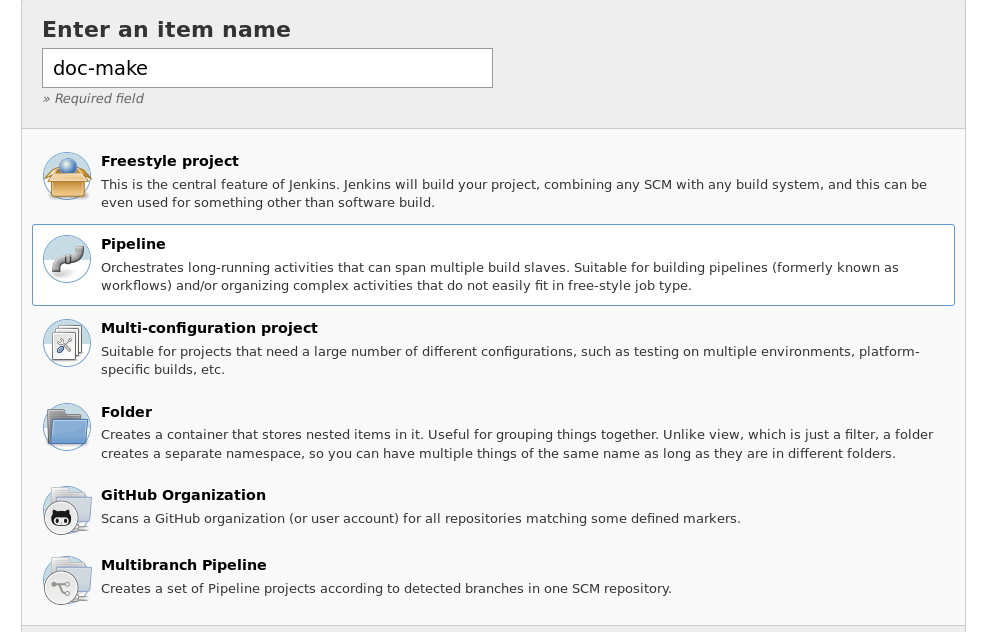
\includegraphics[width=\textwidth,height=0.6\textwidth]{images/jenkins.png}

  \subsection{安裝與基本}
  安裝現在非常簡單,在 https://jenkins.io/download/
  可以用docker 去啟動一個jenkins的docker appliance ,jenkins小組會在docker hub 
  維護 jenkins/jenkins:lts 這個image,只要
  \begin{verbatim}
# docker pull jenkins/jenkins:lts
# docker run -p 8080:8080 -p 50000:50000 jenkins/jenkins:lts
  \end{verbatim}
  或者真的自己裝一個,以我的 debian 來說,只要先裝curl 與 apt-transport-https,然後
  \begin{verbatim}
# curl -fsSL https://pkg.jenkins.io/debian-stable/jenkins.io.key | sudo apt-key add -
  在/etc/source.list加上下面這行
  deb https://pkg.jenkins.io/debian-stable binary
# apt-get update; apt-get install jenkins
  \end{verbatim}
  就完成安裝了。
  \\\\
  安裝完會在8080 port上啟動jenkins,跟CUPS一樣很像,所有的起始與維護都在8080 port
  上開始,一開始會換密碼,加上新使用者,安裝default plugins,就啟動了。
  啟動後又有些新名詞要解釋了,這種management software就是這樣,首先他兩個分類
  \begin{itemize}
    \item JOB/ITEM/PROJECT 就是一個名詞而已,總之create item就只是產生新的build
      project 而已,目前我玩2.89.3的create new item有些template,但其實這些
      template 只是好玩而已,裏面的設定隨時都可以自己亂加進去。
    \item view/my view 其實就是group的意思,每個分類都有大分類,create view 就是
      create 一個大分類項,裏面包含很多job/item/project。list view 是每個人都看
      得到的分類結構,這應該要有權限 , my view 就是自己的整理分類。
  \end{itemize}
  好了現在先create item,目前default 有以下template讓你選並填入project相關資訊
  \begin{itemize}
    \item freestyle 就比較簡單straigforward的tasks資訊輸入。
    \item pipeline 建立pipeline, 這在下面說明。
    \item multi-configuration
    \item folder
    \item github organization 在github上可以建立所謂organization, 就是私人的小組。
      這是跟github溝通用的設定。我記得也有bitbucket的但要額外安裝plugin。
    \item multibranch pipeline 多branch的pipeline
  \end{itemize}
  先選freestyle 最簡單。裏面有GUI設定 git server在哪裡,build跟build間的關係等
  等,然後其實我們很多都只是用build那個步驟的 execute shell 跑我們要的build
  script而已。
  \\\\
  我們還是先看需求
  \begin{itemize}
    \item 整組人員能夠用原本公司內的帳號密碼就login, 這需要LDAP
    \item 管理人員可以有權限設定誰能login誰不能login, 例如公司會計人員就沒必要能
      login
    \item 要能跟source control連結,一但有人trigger build,就能去相關 git/svn 抓
      出相關 branch,啟動一個 build
    \item 要能跟testing report工具連結,一旦測試失敗則這個build也是失敗的。
    \item 要能GUI上debug流程的錯誤在哪。
    \item 能夠發mail, 通知大家結果。
    \item 最好能有pipeline執行不同工作,例如 build, static analysis, automation
      test 等等是可以分開的不同階段的執行,一旦一個完成,別的project可以進入
      pipeline的執行。
    \item build 完後,能在GUI上抓到images。
  \end{itemize}

  \subsection{更多的configuration}
  global system configuration裏面可能 pipeline 是比較新的名詞,其他的就很一般,
  executor就是同時jenkins可以去跑的process數目。
  label就只是別名,可以用這別名來識別操作機器node。
  workspace就是git clone啦,build, testing的目錄,應該是藏在/var/run/jenkins。
  \\\\
  pipeline 就是跟computer architecture上的一樣,完成一件事情需要多階段的tasks,
  從拉出source, build, test到最後deploy到真的機器上,算是生產線流程。
  jenkins管理pipeline,甚至jenkins忽然死掉時,pipeline 的重啟都是自動的。
  pipeline 必須用所謂他的 pipeline dsl語言定義,寫到一個叫Jenkinsfile檔案,
  也有所謂 blue ocean plugin 用GUI輸入參數就幫你輸出一個Jenkinsfile檔案。
  \\\\
  credential configuration 主要是設定其他服務的 uid/password, 像git, slave node
  , email等等服務。 store 與 domain是他分類的大項, 內定store就是master node的
  hostname, 有一個內定 domain 叫 global 是所有的機器都可以用的,自己新創的domain
  裏面可以設定specification, 讓某些機器或設定可以使用而已。就這樣。credential
  的種類有username/password 就是要輸入uid/password的,或者
  ssh Username with private key, 就是使用ssh-keygen產生.ssh/id\_rsa 
  .ssh/id\_rsa.pub 然後把 public key 丟到對方去的,所以輸入是uid/private key,
  ssh-keygen建造時有輸入passphrase,就要輸入jenkins,沒有就沒有。其他方法就是
  有的certificate的方式。certificate說穿了就是public key + 一堆資訊而已。
  \\\\
  manage node, node master 與 slave node 是可以有很多台 build machines 管理,
  其實我很討厭Java, 根本就是resource老饕,所以光裝一台jenkins,很快資源就被吃光
  了,要有其他build machine給他揮霍。剛裝好的jenkins是master node, 主jenkins機器
  ,他可以透過 ssh 控制slave node來完成build, testing 工作,所以我們可
  以在manage node裏面多設幾台 slave node 來讓 master node 來玩他們。說穿了就是
  用 scp 先copy slave.jar 到slave node,然後 ssh 到 slave node 跑slave.jar 而已
  。實際操作時,master node 只是做 conifugraiton 與backup而已,slave node 才是
  真正build, run test的地方,因此 slave node 要先裝好 java,credential
  可以用username/password的方法,但大部分的人是用 privae public key 的方法。
  所以如果是用 root 跑build, copy master node 上 ssh-keygen產生的id\_rsa.pub 到
  slave node 的 /root/.ssh/authorized\_keys, 由於jenkins的內定安裝 Home 是在
  /var/lib/jenkins,所以master node 的 id\_rsa 應該是在/var/lib/jenkins/.ssh 下
  當然如果slave node不是用root跑build job,那就要slave node建立新帳號,把
  id\_rsa.pub放到對的位置。
  \\\\
  create new node選permanent agent, 然後slave node 的remote root directory要改掉
  , 在launch method裏面選"Launch agents via SSH" 然後可以加上creditial後,選他
  就可以了。 至於文件的什麼agent, label就不用去管他了,label只是slave node的別名
  , agent就是那個 ssh 跑起來的session而已。 只是jenkins蠻阿呆的,如果沒有連過
  slave node, .ssh/known\_host沒有slave node資訊,launch agent就會失敗。所以要
  先變身jenkins, 然後 ssh slave node一遍寫進master的known\_host。
  \\\\
  git server的整合,基本git的整合蠻簡單的,這邊是要說明github, bitbucket的整合
  ,我們在前面github, bitbucket時,已經先建立了我們的account,
  \\\\
  user configuration, user 的存取權限

\section{sonarQube}
  sonarQube是個對整體code quality品質統計的一個監督軟體,這通常是經理以上人員
  才有興趣的東西,例如發現為什麼GUI的bugs特別多,或者某方面的分類統計上有異常
  的多或少,根據這些資料來調整組裡的管理事宜。我們公司用這也很多年了,well,
  \href{https://www.sonarqube.org/downloads/}{下載community free版本},也要
  \href{https://openjdk.org/}{下載 openjdk},他也有 container 可以裝,不用
  自己裝這裝那的。
  \begin{itemize}
    \item 解開 openjdk 到 \$HOME/opt/
    \item export JAVA\_HOME=\$HOME/opt/jdk-21.0.2/
    \item export SONAR\_JAVA\_PATH=\$HOME/opt/jdk-21.0.2/bin/java
    \item 啟動 postgreSQL 跟設定 username, password
    \item bin/linux-x86-64/sonar.sh start
    \item http://localhost:9000
    \item 內定uid/passwd : admin/admin
  \end{itemize}
\section{其他}
  共筆wiki與小組文件可以用 wiki.org, readthedocs.org,
  小組文件通常是一些組裡的規定,資訊,例如寫code的convention, lab機器在哪裡
  IP是多少等等,這些可以用wiki的方式讓大家寫作與分享。readthedocs.org是
  另一個文件產生器網站,用rst語法能產生目錄與文件,他是opensource的,所以能
  裝一個到自己內部來使用。
  \\\\
  https://jfrog.com/artifactory/
  \\\\
  artifactory是一個binary release的管理工具。我們公司內部也有用在各組的
  release 管理,這主要用在對內的發佈,正式公司對外發佈有我們的另外一套,
  不過我對binary的管理不是很感興趣,主要是傳統上我們就放在自家file system 
  上就好了,主要是版本,不同images形式,名稱的分門別類然後他是有GUI的就這樣
  , 那公司有可能想要統一中央集權管理這些內部binary release,又我們DE, QA, 
  PM, OPs, Marketing 等組的介面參考,可以很快方便找到,也有人在推用就是。
  \\\\
  https://www.ansible.com/
  \\\\
  ansible是一個自動deploy的工具,但...就是寫個像pipeline定義的檔,
  用的是yml格式,用ssh在一堆遠端執行命令, 通常這些
  工具的好處是有 GUI 操作,統計圖表等等。這種控制非常多台node的程式也叫
  orchestrator, 交響樂的指揮家。傳統上很多公司也都有提供自家的
  orchestration軟體來控管自家的機器,只是現在storage, network等機器都已經
  被opensource virtualization取代,幾乎這些公開的介面已成為標準,所以慢慢
  我想opensource的orchestration軟體最後也會把傳統公司給吃掉的。以前老工程
  師會個私有公司的工具就好像吃不完,現在要熟悉opensource工具組才行。
\section{結語}
  其實由於幾十年來,太多亂七八糟的工具了,所以有人在推,也有很多組用傳
  統的工具,就像code review一樣,我們內部其實從早期自己寫的到review board,
  gerrit, bitbucket, github等一直轉換,現在應該都是 github, bitbucket 了,
  大概也不會再有新工具了。
  \\\\
  不過很多問題的解決不在於使用什麼工具就解決的了,人與人的溝通,衝突,不協
  調問題都在於人的貪嗔痴,這些東西不可能像那些表面所想的用什麼物質,什麼步驟
  就能改變,就能讓大家想的跟你想的一樣,導入什麼工具就萬事ok,如果能,那人就
  不叫人了。一個startup要成功還是要有真正尖端技術,10人以下同心同德專業團隊
  ,做起來後從大眾口袋中拿出一毛錢,賺大錢後才有可能去搞這些大堆頭的管理遊戲
  。

\end{document}
